% Template de Apostila do Campus Cachoeiro do Instituto Federal do Espírito Santo
% Autor: Prof. Ricardo Maroquio
% Baseado no Template "The Legrand Orange Book" Version 3.1 (February 18, 2022)
%
% License:
% CC BY-NC-SA 4.0 (https://creativecommons.org/licenses/by-nc-sa/4.0/)
%
%----------------------------------------------------------------------------------------
%	PACKAGES AND OTHER DOCUMENT CONFIGURATIONS
%----------------------------------------------------------------------------------------

\documentclass[
	11pt, % Default font size, select one of 10pt, 11pt or 12pt
	fleqn, % Left align equations
	a4paper, % Paper size, use either 'a4paper' for A4 size or 'letterpaper' for US letter size
        twoside,
	%oneside, % Uncomment for oneside mode, this doesn't start new chapters and parts on odd pages (adding an empty page if required), this mode is more suitable if the book is to be read on a screen instead of printed
]{ifescai}

% Book information for PDF metadata, remove/comment this block if not required 
\hypersetup{
	pdftitle={Apostila de Desenvolvimento Web}, % Title field
	pdfauthor={Prof. Dr. Ricardo Maroquio}, % Author field
	pdfsubject={Programação de Computadores}, % Subject field
	pdfkeywords={html, css, bootstrap}, % Keywords
	pdfcreator={LaTeX}, % Content creator field
}

\setminted[html]
{frame=leftline,
framesep=2mm,
baselinestretch=1.2,
bgcolor=white,
fontsize=\small,
linenos}

\addbibresource{sample.bib} % Bibliography file

\definecolor{ocre}{RGB}{243, 102, 25} % Define the color used for highlighting throughout the book
\definecolor{darkgreen}{RGB}{0,64,0}

\chapterimage{chapter_bg.pdf} % Chapter heading image
\chapterspaceabove{5.71cm} % Default whitespace from the top of the page to the chapter title on chapter pages
\chapterspacebelow{5cm} % Default amount of vertical whitespace from the top margin to the start of the text on chapter pages

%----------------------------------------------------------------------------------------

\begin{document}

\counterwithin{listing}{chapter} % faz a numeração dos algoritmos reiniciar a cada capítulo

%----------------------------------------------------------------------------------------
%	TITLE PAGE
%----------------------------------------------------------------------------------------

\titlepage % Output the title page
	{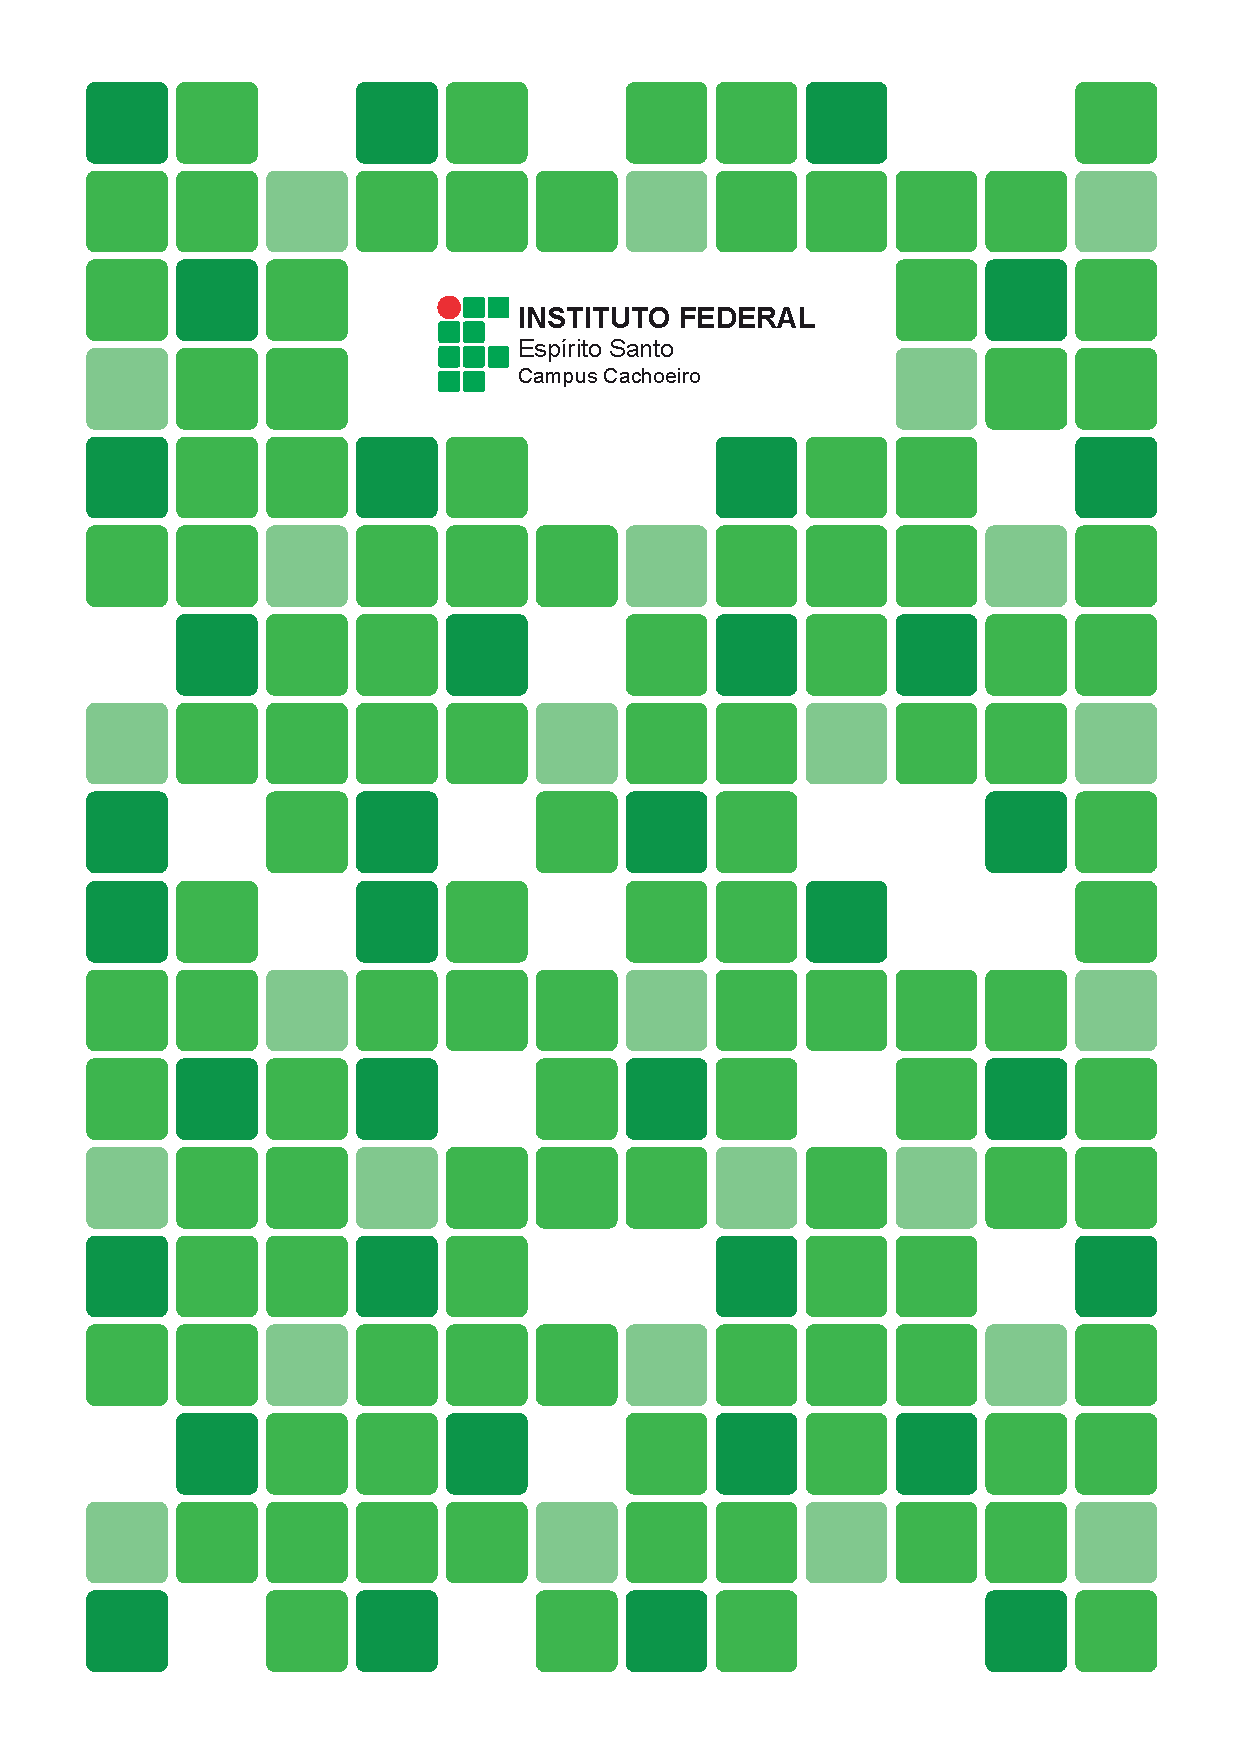
\includegraphics[width=\paperwidth]{cover_bg2.pdf}} % Code to output the background image, which should be the same dimensions as the paper to fill the page entirely; leave empty for no background image        
	{ % Title(s) and author(s)
		\centering\sffamily % Font styling
		{\Huge\bfseries Desenvolvimento Web\par} % Book title
		\vspace{4pt} % Vertical whitespace
		{\LARGE Bacharelado em Sistemas de Informação\par} % Subtitle
		\vspace{24pt} % Vertical whitespace
		{\huge\bfseries Prof. Ricardo Maroquio\par} % Author name
	}

%----------------------------------------------------------------------------------------
%	COPYRIGHT PAGE
%----------------------------------------------------------------------------------------
\sffamily
\normalsize
\setlength{\parskip}{12pt}
\thispagestyle{empty} % Suppress headers and footers on this page

~\vfill % Push the text down to the bottom of the page

\noindent Copyright \copyright\ 2023 Ricardo Maroquio\\ % Copyright notice

\noindent \textsc{Instituto Federal do Espírito Santo}\\ % Publisher
\noindent \textsc{Campus Cachoeiro}\\ % Publisher


\noindent Disponível para download em:\\
\noindent \textsc{\href{https://www.maroquio.com/}{http://maroquio.com}}\\ % URL
\begin{spacing}{1.5}
\noindent Esta apostila está sob a licença \textit{Creative Commons Attribution-NonCommercial 4.0}. Você só pode usar esse material se concordar com essa licença. Você pode acessar a licença em \url{https://creativecommons.org/licenses/by-nc-sa/4.0}. A menos que seja aplicável por lei ou acordado por escrito, material digital sob esta licença deve deve ser distribuído \textsc{``como está'', sem garantias ou condições de nenhum tipo}. Para maiores informações sobre o uso deste material, consulte a licença disponível no link supracitado.\\

\noindent \textit{Fevereiro de 2023} % Printing/edition date

%----------------------------------------------------------------------------------------
%	TABLE OF CONTENTS
%----------------------------------------------------------------------------------------
\renewcommand*\contentsname{Sumário}

\renewcommand{\listfigurename}{Lista de Figuras}

\renewcommand{\listtablename}{Lista de Tabelas}

\renewcommand{\listoflistingscaption}{Lista de Exemplos de Código}

\renewcommand{\listingscaption}{Exemplo de Código}

\setcounter{tocdepth}{1}

%https://latex-tutorial.com/caption-customization-latex/
\captionsetup{singlelinecheck=false, font={sf}, labelfont=bf, justification=raggedright, size=small}

\captionsetup[listing]{singlelinecheck=false, font={sf}, labelfont=bf, justification=raggedright, size=small}

\pagestyle{empty} % Disable headers and footers for the following pages

\tableofcontents % Output the table of contents

\listoffigures % Output the list of figures, comment or remove this command if not required

%\listoftables % Output the list of tables, comment or remove this command if not required

\listoflistings % Output the list of code examples, comment or remove this command if not required

\pagestyle{fancy} % Enable default headers and footers again

\cleardoublepage % Start the following content on a new page

%----------------------------------------------------------------------------------------

\part{Parte I: HTML}

\chapterimage{chapter_bg.pdf} % Chapter heading image
%\chapterspaceabove{6.75cm} % Whitespace from the top of the page to the chapter title on chapter pages
%\chapterspacebelow{7.25cm} % Amount of vertical whitespace from the top margin to the start of the text on chapter pages

\chapter{Introdução}

O mundo tem hoje mais de 4.7 bilhões de usuários de internet, sendo que cada usuário padrão passa cerca de 6 horas e meia por dia navegando. Conquistar um pouco da atenção desse usuário, seja através de um site ou de uma página em rede social, deixou de ser algo opcional. 

Não é à toa que existem mais 1.8 bilhão de sites na web atualmente. Consequentemente, nunca houve tanta demanda por profissionais capazes de criar e administrar sites. Se você quer aproveitar essa oportunidade aprendendo a criar e a publicar sites, você está no lugar certo. Vale ressaltar que este material é totalmente voltado para iniciantes, isto é, para quem realmente não sabe nada sobre criação de sites. 

\section{O Funcionamento de um Site}

Nesta seção, eu vou explicar os princípios básicos de funcionamento de um site, para que, antes de começar a codificar, você entenda como as coisas funcionam nos bastidores. Essa compreensão é imprescindível para que você consiga criar sites de qualidade de jeito certo. 

Um site é composto por uma ou mais páginas de hipertexto. Diferentemente de um texto comum, uma página de hipertexto corresponde a uma página que pode conter textos, imagens e elementos multimídia de forma combinada para comunicar alguma ideia. Mas o principal diferencial de uma página de hipertexto é que ela pode conter ligações com outras páginas, de forma que o leitor possa navegar para essas outras páginas através dessas ligações, que são chamadas de hiperlinks, ou simplesmente \textit{links}. A figura \ref{fig:siteslinked} apresenta exemplos fictíticos de sites que possuem hiperlinks conectando-os.

\begin{figure}[htbp!]
    \centering
    \includegraphics[width=0.6\textwidth]{Images/chapter01/sites_linkados.png}
    \caption{Sites conectados através de hiperlinks.}
    \label{fig:siteslinked}
\end{figure}

Nos bastidores, para que o navegador consiga exibir o conteúdo da forma como você está acostumado a ver quando navega pela web, um texto contendo um conjunto de instruções deve indicar ao navegador \textbf{quais} elementos devem ser exibidos e \textbf{como} esses elementos devem ser exibidos. Essas instruções interpretadas pelo navegador são chamadas de \textbf{códigos}, que nada mais são do que textos escritos em um padrão que chamamos de \textbf{linguagem}. Toda página de um site, basicamente, é uma combinação de códigos escritos em três linguagens diferentes: HTML, CSS e Javascript, como mostra a figura \ref{fig:sitescodigo}.

\begin{figure}[htbp!]
    \centering
    \includegraphics[width=1\textwidth]{Images/chapter01/site_codigos.png}
    \caption{Os códigos que compõem uma página de hipertexto.}
    \label{fig:sitescodigo}
\end{figure}

A primeira linguagem, \textbf{HTML}, é uma sigla para \textit{HyperText Markup Language}, traduzindo, Linguagem de Marcação de Hipertexto, ou seja, é uma linguagem de \textbf{marcação}. Em síntese, ela é a responsável por definir \textbf{quais} elementos serão exibidos em uma determinada página. \textbf{CSS} é outra sigla, que quer dizer \textit{Cascading Style Sheets}, ou folhas de estilo em cascata, portanto, é uma linguagem de \textbf{folhas de estilo}, ou uma linguagem de definição de estilos. Ela é responsável por definir \textbf{como} os elementos de conteúdo serão mostrados.

É através da linguagem CSS que apresentamos um mesmo conteúdo de forma alegre, de forma séria, de forma suave, chamativa etc. Resumindo, as definições de estilos CSS é que nos permitem mudar a forma como um conteúdo é exibido, ou seja, o visual do conteúdo.

Diferentemente de HTML e CSS, \textbf{Javascript} é uma linguagem de \textbf{programação}. Ela pode ter diferentes propósitos em uma página web e, pelo fato de ser uma linguagem de programação, requer conhecimentos de lógica de programação. Uma abordagem profunda da linguagem Javascript está fora do escopo deste material. Veremos apenas qual é o papel da linguagem Javascript em uma página web.

Primeiramente, é importante ressaltar que, para construir sites, não somos obrigados a usar Javascript. Na verdade, basicamente, somente sites que possuem interação com o usuário e/ou efeitos visuais avançados é que requerem o uso de Javascript . No final deste capítulo, eu voltarei a falar um pouco mais sobre Javascript, só para dizer como ele pode contribuir para o funcionamento de um site. Temos que ver algumas coisas antes para que você entenda melhor o papel do código Javascript.

Bem, essa combinação de HTML, CSS e Javascript forma o código-fonte de uma página web. Você consegue ver o código-fonte de qualquer página web clicando com o botão direito do mouse sobre a página em um navegador qualquer e selecionando a opção “Exibir código-fonte da página”, ou “Ver código-fonte da página”, ou alguma coisa parecida com isso (depende do navegador). 

A princípio, o código-fonte que será exibido pode parecer algo meio assustador, mas em pouco tempo você já será capaz de compreender boa parte dele. O código-fonte de uma página web geralmente fica distribuído em mais de um arquivo. Na verdade, é uma boa prática separar em arquivos distintos os códigos HTML, CSS e Javascript. Pode acontecer, inclusive, de cada tipo de arquivo ser mantido por um programador diferente.

Normalmente, uma página contém apenas 1 arquivo HTML, mas pode estar associada a vários arquivos CSS e a vários arquivos Javascript. Os arquivos HTML podem ter a extensão ``htm'' ou ``html'', enquanto os arquivos CSS possuem a extensão ``css'', e os arquivos Javascript possuem a extensão ``.js''.

Quanto ao código CSS, é comum ter um arquivo para estilizar botões, outro para estilizar o leiaute da página, outro para estilizar os textos, entre outros mais. Separar esses códigos CSS em arquivos diferentes pode ajudar a melhorar a organização do código-fonte de um site como um todo. Portanto você poderia criar um arquivo CSS para estilizar botões, outro para o leiaute, outro para a tipografia e assim por diante.

Outra observação importante é que as páginas de um mesmo site normalmente possuem um mesmo estilo. Geralmente usam as mesmas cores, a mesma tipografia, o mesmo leiaute, o mesmo estilo de cabeçalho e rodapé, entre outras coisas. Portanto, é comum que os mesmos arquivos CSS sejam compartilhados entre diferentes páginas web.

Assim, se você quiser mudar a tipografia usada em todas as páginas do site, basta ir ao arquivo CSS que contém essa formatação e mudar as propriedades de fonte desejadas. Assim, o site inteiro passará a ser mostrado com as novas definições de fonte. Pense em como isso facilita a manutenção de um site!

Quanto ao código Javascript, também é comum que as páginas compartilhem os mesmos códigos. É possível ter um código para mostrar uma janela com mensagem, para animar um elemento da página, para atualizar apenas uma parte da página, entre outros. Se determinado código Javascript é específico de uma página, recomenda-se separá-lo em um arquivo que será vinculado exclusivamente à página a que pertence. Isso evita que outras páginas carreguem códigos Javascript que não sejam necessários para ela. Assim como ocorre com CSS, é comum que um mesmo arquivo Javascript esteja vinculado a diferentes páginas, pois elas podem ter funcionalidades comportamentais em comum.

\subsection{Páginas Estáticas e Dinâmicas}

Os arquivos que compõem o código-fonte de uma página podem ter origem de duas fontes diferentes: podem ser arquivos prontos, que simplesmente serão baixados do servidor web que hospeda o site; ou podem ser gerados por um programa especial chamado de aplicação web, que roda no servidor web e que gera o código-fonte da página sempre que ela é solicitada por um usuário.

Quando as páginas de um site são totalmente compostas por arquivos prontos, dizemos que o site é estático. Quando as páginas (ao menos algumas delas) são geradas por uma aplicação web, dizemos que o site é dinâmico. É muito comum ter sites que possuem páginas estáticas e páginas dinâmicas. A figura \ref{fig:sitesestdyn} mostra como os sites estáticos e dinâmicos são servidos ao navegador do usuário.

\begin{figure}[htbp!]
    \centering
    \includegraphics[width=1\textwidth]{Images/chapter01/site_est_dyn.png}
    \caption{Sites estáticos e dinâmicos.}
    \label{fig:sitesestdyn}
\end{figure}

Normalmente, o código que é gerado dinamicamente por uma aplicação web é aquele relacionado ao conteúdo da página, ou seja, o código HTML. Os códigos CSS e Javascript raramente são gerados dinamicamente. Normalmente eles são criados de forma estática por um programador e permanecem intocados ao longo de toda a vida da aplicação web. Quando é necessário atualizar a aparência do site ou incluir novas funções Javascript para executar alguma tarefa adicional, os arquivos podem ser modificados por alguém, mas depois da modificação eles continuam estáticos no servidor, ou seja, eles \textbf{não serão gerados} pela aplicação web.

Um site estático tem a característica de não demandar atualizações com muita frequência. Um site que tenha o propósito de contar a história do Brasil, por exemplo, vai ter um conteúdo que dificilmente será alterado. Se houver necessidade de alteração, a frequência será tão baixa que basta fazer a alteração diretamente nos arquivos HTML. Não vale a pena criar uma aplicação web acessando um banco de dados para gerar conteúdo se tal conteúdo muda somente uma vez por ano, por exemplo. Neste caso, vale a pena abrir o arquivo HTML em um editor e fazer a modificação diretamente no arquivo correspondente ao conteúdo da página. 

\subsection{O Conceito de Requisição de Página}

Quando um endereço de um site é digitado na barra de endereços do navegador, a primeira coisa a ser baixada pelo navegador é o código HTML. Como já mencionado, esse código pode vir de um arquivo estático ou pode ser gerado por uma aplicação web que esteja rodando no servidor. Esse código HTML normalmente contém referências para os demais arquivos necessários para a página ser renderizada. Aí entram os arquivos com códigos CSS e Javascript, os arquivos de imagens e arquivos de outras mídias que façam parte da página. De posse do endereço desses arquivos associados, o navegador faz o download de cada um deles e renderiza a página.

A figura \ref{fig:reqpagina} apresenta um diagrama que mostra desde o momento em que o usuário digita o endereço de um site no navegador até o momento em que o navegador exibe a página para o usuário. Ressalto que esse diagrama é uma abstração do processo real. Isso quer dizer que algumas detalhes que acontecem nos bastidores foram suprimidos ou simplificados visando facilitar o entendimento do processo.

\begin{figure}[htbp!]
    \centering
    \includegraphics[width=1\textwidth]{Images/chapter01/digrama_requisicao.png}
    \caption{Diagrama de uma requisição de página pelo navegador.}
    \label{fig:reqpagina}
\end{figure}

Na figura \ref{fig:reqpagina}, tudo começa com o usuário informando uma URL na barra de endereços do navegador. Acontece que, para acessar um servidor web, é necessário saber seu número IP. A sigla IP vem de \textit{Internet Protocol}, ou ``protocolo de internet''. O número IP de um servidor é mundialmente único, ou seja, ele é um endereço exclusivo do servidor em toda a internet.

Os nomes de domínio, como google.com.br, maroquio.com.br e youtube.com.br, são simplesmente apelidos para endereços IP de um servidor. O fato de usarmos nomes de domínio em vez de endereços IP numéricos é pelo fato dos nomes serem humanamente mais fáceis de se memorizar e mais fáceis de serem associados a entidades do mundo real. Em síntese, além de ser mais fácil memorizar um nome do que um número que pode ter até 12 dígitos, o nome do domínio pode ser composto pelo próprio nome da entidade que ele representa, facilitando ainda mais a memorização. O domínio microsoft.com é um exemplo disso.

Mas como o navegador faz para descobrir o endereço IP de um servidor web a partir de um nome de domínio? Na verdade, o navegador consulta primeiro um servidor DNS. DNS significa \textit{Domain Name System}, ou ``Sistema de Nomes de Domínios''. Esse servidor contém uma tabela que mapeia nomes de domínios para endereços IP. Portanto, quando ele recebe um pedido de consulta de um domínio, ele percorre essa tabela e retorna o IP do domínio consultado.

Existem vários servidores DNS espalhados pelo mundo, e essa tabela é atualizada com certa frequência para refletir a inclusão de novos domínios que tenham sido registrados, bem como a remoção de domínios que não estão mais ativos e a alteração de domínios que ocorre quando um site é mudado de um servidor web para outro.

Uma vez que o endereço IP do servidor web tenha sido obtido, uma requisição HTTP é feita ao servidor web correspondente ao IP em questão. Não se assuste com o termo ``requisição HTTP''. Isso nada mais é do que o seu navegador fazendo um pedido de algum recurso para o servidor web usando uma linguagem que os dois conhecem bem, que é o protocolo \textbf{HTTP}. 

A sigla HTTP, que você já deve ter visto no início do endereço de vários sites, quer dizer \textit{Hyper Text Transfer Protocol}, ou, ``Protocolo de Transferência de Hipertexto''. Lembra que eu falei que as páginas de um site são hipertextos? Pois é! Por isso o nome do protocolo diz respeito à transferência de hipertexto.

Existe uma forma correta de o navegador solicitar uma página de hipertexto a um servidor web. Essa forma é o que chamamos de ``protocolo'', que neste caso é o HTTP. Uma requisição HTTP é composta por vários dados, entre eles, o idioma preferencial do usuário, o nome de domínio onde está o recurso solicitado e o nome do recurso que está sendo solicitado. O recurso solicitado por ser um arquivo HTML, CSS, Javascript, ou pode ser um arquivo de imagem qualquer, ou, pode ser um nome de recurso que será gerado por uma aplicação web. O código \ref{code_req} mostra um exemplo de cabeçalho HTTP para uma requisição ao servidor da Microsoft.

\begin{htmlcode}{Exemplo de cabeçalho de uma requisição HTTP}{code_req}
GET /produtos HTTP/1.1
Host: www.microsoft.com
User-Agent: Mozilla/5.0 (Windows NT 10.0; Win64; x64) Chrome/89.0.4389.82 Safari/537.36
Accept: text/html,application/xhtml+xml,application/xml;q=0.9,image/webp,*/*;q=0.8
Accept-Language: en-US,en;q=0.5
Accept-Encoding: gzip, deflate, br
Connection: keep-alive
\end{htmlcode}


Cada arquivo necessário para a renderização da página gera uma requisição HTTP. Veja que isso tudo acontece em poucos segundos. Lembre-se também de que, quanto menor é o tempo de carregamento de uma página, menos chance ela tem de ser abandonada pelo usuário. Um dos maiores desafios ao se construir um site é o de reduzir o tempo de carregamento das páginas. Ao longo deste material, veremos algumas técnicas que vão ajudar nessa questão.

Continuando no diagrama da figura \ref{fig:reqpagina}, vamos imaginar que o recurso solicitado é uma página dinâmica. Nesse caso, para gerar a página, alguns dados a mais normalmente são necessários, e esses dados costumam ficar armazenados em um banco de dados. Vamos analisar um exemplo real rapidamente. 

A figura \ref{fig:pagsyout} mostra as páginas com detalhes de 3 vídeos do meu canal no YouTube, cada uma com seu respectivo endereço. Veja que os endereços são bem parecidos. Todos começam com HTTPS, que nada mais é do que uma versão segura do protocolo HTTP. Em seguida vem o nome do domínio, nesse caso, \textit{www.youtube.com}. Depois vem o nome do recurso que estamos acessando, que é a página \textit{watch}; e, por fim, temos uma interrogação (?) seguida de um ``V=XXXXXXX'', onde o \textit{X} pode ser qualquer caractere alfanumérico. 

\begin{figure}[htbp!]
    \centering
    \includegraphics[width=1\textwidth]{Images/chapter01/pags_youtube1.png}
    \caption{Páginas de vídeos específicos do YouTube.}
    \label{fig:pagsyout}
\end{figure}

Isso que vem depois da interrogação na URL do vídeo é um parâmetro. Esse parâmetro é o identificador do vídeo que está sendo exibido. É como se fosse o ``CPF'' do vídeo. Daqui a pouco vamos estudar mais sobre esse identificador. Veja que o estilo da página é o mesmo para os três vídeos. Isso caracteriza bem as páginas geradas dinamicamente. Elas têm um estilo praticamente idêntico, incluindo fonte de letra, cores, leiaute, botões etc., e alguns dados mudam de uma para outra.

Tente identificar, na figura \ref{fig:pagsyout}, quais dados mudam de uma página para outra. Vamos lá. Temos a imagem de capa do vídeo, o título, a quantidade de visualizações, a data de publicação, a quantidade de likes e dislikes, e a descrição. Esses dados são obtidos de um banco de dados no servidor do YouTube. Se você nunca estudou banco de dados, não se preocupe, porque é algo desnecessário para esta fase do aprendizado. A figura \ref{fig:pagsyoutmarcado} mostra os dados dinâmicos contornados por retângulos alaranjados.

\begin{figure}[htbp!]
    \centering
    \includegraphics[width=1\textwidth]{Images/chapter01/pags_youtube2.png}
    \caption{Páginas de vídeos específicos do YouTube com dados dinâmicos destacados.}
    \label{fig:pagsyoutmarcado}
\end{figure}

Tudo que vem depois de uma interrogação em uma URL é considerado parâmetro. Pode acontecer de uma mesma URL ter vários parâmetros separados pelo símbolo \textbf{\&}. O valor desse parâmetro ``V'' funciona como um identificador. Com ele é possível encontrar um determinado vídeo no banco dados de vídeos do YouTube. Se você já estudou banco de dados, já deve ter feito a associação desse parâmetro ``V'' com a chave primária de uma tabela que guarda os dados dos vídeos.

A aplicação web do YouTube foi programada para usar esse parâmetro e consultar um banco de dados para buscar os dados específicos do vídeo em questão. Em seguida, a aplicação web combinou esses dados com um modelo genérico de página HTML criado por algum designer do YouTube, gerando o conteúdo e enviando de volta ao navegador do usuário através de uma resposta HTTP. 

Esse modelo de página HTML já contém as referências para arquivos CSS, Javascript, imagens e o que mais for necessário para renderizar a página do vídeo por completo. Portanto, conforme já estudamos, logo que recebe esse conteúdo HTML, o navegador já faz novas requisições ao servidor do YouTube para buscar os outros arquivos necessários para a renderização da página. Depois de baixar todos os arquivos, a renderização da página é concluída.

\subsection{Um Pouco Mais Sobre Javascript}

Agora vamos voltar a falar do código Javascript que vimos rapidamente. Basicamente, ele desempenha dois papéis em uma página de hipertexto. O primeiro deles é a modificação de conteúdo mediante a ocorrência de algum evento. Por exemplo, se o usuário clicar em um botão, eu quero que determinado menu seja expandido ou que uma imagem sofra um zoom. Isso quer dizer que, com Javascript, você consegue manipular os elementos HTML que estão renderizados em uma página, incluindo seus estilos CSS. Isso pode deixar a página um pouco mais interativa.

O segundo papel desempenhado pelo Javascript é o de carregar conteúdo do servidor web em segundo plano, permitindo atualizar partes da página sem a necessidade de requisitar toda a página novamente. Como exemplo, imagine um site que mostre o placar de jogos de futebol em tempo real, como na figura \ref{fig:site_placar}. Para que a experiência do usuário seja a melhor possível, é interessante atualizar o placar no máximo a cada 1 segundo, senão o usuário escuta o grito de gol do vizinho e só 30 segundos depois o placar muda para ele, gerando uma péssima experiência.

\begin{figure}[htbp!]
    \centering
    \includegraphics[width=1\textwidth]{Images/chapter01/site_placar.png}
    \caption{Atualização parcial de página usando Javascript em segundo plano.}
    \label{fig:site_placar}
\end{figure}

Acontece que recarregar toda a página novamente a cada segundo é algo computacionalmente custoso, e milhares de usuários fazendo isso ao mesmo tempo sobrecarregaria o servidor. Neste caso, usando Javascript, é possível criar um temporizador que dispare uma função a cada 1 segundo, sendo que essa função faz uma consulta ao servidor web usando o endereço de um recurso que retorna somente o placar do jogo em questão. Em seguida, a função vai no elemento HTML que mostra o placar na página e atualiza seu conteúdo com o novo valor do placar recebido do servidor. Isso tudo é realizado em segundo plano pelo navegador e evita o recarregamento total da página.

Apesar de Javascript ser um recurso útil, principalmente para a criação de sites dinâmicos, o foco deste material é a criação de sites estáticos. Na verdade, independentemente do site ser estático ou dinâmico, o código que chega no navegador para ser renderizado tem exatamente as mesmas características, ou seja, tipicamente temos o código HTML para definir o conteúdo e o código CSS para definir a aparência do site. Eventualmente, podemos ter código Javascript para desempenhar algum dos papéis que mencionei. Isso quer dizer que, para criar sites dinâmicos, o primeiro passo é aprender a criar sites estáticos, que é o nosso propósito aqui.

\section{Exercícios Propostos}

Essa série de exercícios envolve os conceitos abordados neste capítulo e também \textbf{pode demandar alguma pesquisa}. Reserve um tempo e um local adequados para fazer os exercícios sem distrações. Assim você absorverá muito mais o conteúdo estudado.

\begin{exercise}
Quais são os 3 tipos de códigos básicos de uma página de hipertexto? Explique para que serve cada um dos tipos.
%R: Os três tipos de códigos básicos de uma página de hipertexto são HTML (HyperText Markup Language), CSS (Cascading Style Sheets) e JavaScript. O HTML define a estrutura e o conteúdo da página, o CSS define a aparência visual da página e o JavaScript permite a criação de interações e funcionalidades dinâmicas na página.
\end{exercise}

\begin{exercise}
Quantos arquivos CSS e Javascript podem estar vinculados a uma mesma página de hipertexto? Justifique sua resposta.
%R: Não há um número máximo ou mínimo de arquivos CSS e JavaScript que podem estar vinculados a uma página de hipertexto. Depende da complexidade da página e da quantidade de estilos e funcionalidades necessárias. É comum que uma página tenha pelo menos um arquivo CSS e um arquivo JavaScript para definir sua aparência e comportamento básico. No entanto, é possível vincular quantos arquivos CSS e JavaScript forem necessários para atender às necessidades da página. É importante lembrar que quanto mais arquivos estiverem vinculados, mais tempo será necessário para carregar a página, o que pode afetar negativamente a performance da página. Por isso, é importante otimizar o uso dos arquivos e minimizar o número de arquivos vinculados, se possível.
\end{exercise}

\begin{exercise}
É possível diferentes páginas de hipertexto terem vínculo com os mesmos arquivos Javascript e CSS? Justifique sua resposta.
%R: Sim, é possível que diferentes páginas de hipertexto tenham vínculo com os mesmos arquivos CSS e JavaScript. Isso é feito para que o mesmo estilo e comportamento sejam aplicados a diferentes páginas, tornando mais fácil a manutenção e atualização dos estilos e funcionalidades dessas páginas. Além disso, isso permite a reutilização de código e a melhor performance de carregamento da página, já que os arquivos CSS e JavaScript são armazenados em cache pelo navegador e não precisam ser carregados novamente a cada nova página.
\end{exercise}

\begin{exercise}
Descreva a diferença entre uma página de hipertexto estática e uma dinâmica, pontuando as vantagens e desvantagens de cada um dos dois tipos.
%R: Uma página de hipertexto estática é uma página que apresenta o mesmo conteúdo para todos os usuários e para todas as visitas. O conteúdo é armazenado no servidor e é enviado para o navegador do usuário sem qualquer alteração. Já uma página de hipertexto dinâmica é uma página cujo conteúdo pode ser modificado em tempo real, dependendo das ações do usuário ou de outros fatores, como informações obtidas de um banco de dados. O conteúdo da página é gerado dinamicamente no servidor e é enviado para o navegador do usuário a cada requisição. Em geral, as páginas dinâmicas oferecem mais interatividade e recursos personalizados do que as páginas estáticas, mas também requerem mais recursos do servidor e podem ser mais lentas em comparação com as páginas estáticas. A escolha entre uma página estática ou dinâmica depende das necessidades e objetivos específicos de cada projeto.
\end{exercise}

\begin{exercise}
Qual é o caminho percorrido por uma requisição HTTP a uma página de hipertexto estática?
%R: O caminho percorrido por uma requisição HTTP a uma página de hipertexto estática é o seguinte: 1) O usuário insere o endereço da página ou clica em um link que o direciona à página. 2) O navegador do usuário envia uma requisição HTTP ao servidor web para solicitar a página. 3) O servidor web recebe a requisição e verifica se a página solicitada está disponível em seus arquivos. 4) Se a página estiver disponível, o servidor envia a página para o navegador do usuário, juntamente com cabeçalhos HTTP que incluem informações adicionais sobre a página, como o tipo de conteúdo e a data da última modificação. 5) O navegador do usuário recebe a página e a renderiza para o usuário. 6) Se a página depende de mais arquivos para ser renderizada, o navegador cria uma nova requisição para cada arquivo necessário. 7) O processo é concluído. A próxima vez que o usuário solicitar a página, o navegador verificará se a versão em cache é a mais recente antes de enviar uma nova requisição ao servidor. Se a versão em cache for a mais recente, o navegador a usará em vez de enviar uma nova requisição.
\end{exercise}

\begin{exercise}
Qual é o caminho percorrido por uma requisição HTTP a uma página de hipertexto dinâmica?
%R: O caminho percorrido por uma requisição HTTP a uma página de hipertexto dinâmica é semelhante ao caminho percorrido por uma requisição a uma página estática, com algumas diferenças adicionais: 1) O usuário insere o endereço da página ou clica em um link que o direciona à página. 2) O navegador do usuário envia uma requisição HTTP ao servidor web para solicitar a página. 3) O servidor web recebe a requisição e processa as informações enviadas pelo usuário ou pelo navegador, se houver. 4) O servidor gera dinamicamente o conteúdo da página com base nas informações recebidas e em dados obtidos de bancos de dados ou outras fontes. 5) O servidor envia a página gerada dinamicamente para o navegador do usuário, juntamente com cabeçalhos HTTP que incluem informações adicionais sobre a página, como o tipo de conteúdo e a data da última modificação. 6) O navegador do usuário recebe a página e a renderiza para o usuário. 7) Se, durante a renderização, outros arquivos forem necessários para renderizar a página, o navegador gera uma nova requisição para cada arquivo necessário. 7) O processo é concluído. A próxima vez que o usuário solicitar a página, o navegador verificará se a versão em cache é a mais recente antes de enviar uma nova requisição ao servidor. Se a versão em cache for a mais recente, o navegador a usará em vez de enviar uma nova requisição.
\end{exercise}

\begin{exercise}
Quais as vantagens da atualização parcial de conteúdo em segundo plano em uma página de hipertexto usando Javascript?
%R: As vantagens da atualização parcial de conteúdo em segundo plano em uma página de hipertexto usando JavaScript incluem: 1) Melhor experiência do usuário: Com a atualização parcial de conteúdo, a página não precisa ser recarregada completamente, o que torna a navegação mais rápida e suave. 2) Maior interatividade: A atualização parcial de conteúdo permite que partes da página sejam atualizadas sem que o usuário precise recarregá-la completamente, o que torna a interação com a página mais rica e intuitiva. 3) Menor uso de largura de banda: Com a atualização parcial de conteúdo, apenas as partes da página que precisam ser atualizadas são transferidas, o que minimiza o uso de largura de banda. 4) Menor sobrecarga no servidor: Com a atualização parcial de conteúdo, o servidor não precisa processar todas as requisições de página, o que minimiza a sobrecarga no servidor. 5) Maior flexibilidade: A atualização parcial de conteúdo permite que as páginas sejam atualizadas dinamicamente sem que o usuário precise recarregá-las completamente, o que torna mais fácil e rápido fazer mudanças na interface da página.
\end{exercise}

\section{Considerações Sobre o Capítulo}

Este capítulo apresentou os fundamentos do funcionamento de um site. Foram apresentados os papéis das linguagens HTML, CSS e Javascript, a diferença de páginas web estáticas e dinâmicas, o conceito e os detalhes básicos de uma requisição HTTP, e um exemplo útil de uso da linguagem Javascript para melhorar a experiência de visualização de um site com atualização parcial em tempo real. No capítulo seguinte, estudaremos a estrutura básica de documentos HTML e CSS.
\chapter{Documentos HTML e CSS}

Este capítulo aborda a estrutura básica dos de documentos HTML e CSS. Veremos como é a hierarquia de elementos de um documento HTML, como se cria um novo elemento, o que são \textit{tags}, atributos e valores de atributos. Veremos também como é o código de um documento CSS básico, com seletores e propriedades para formatação visual de elementos específicos.

\section{Estrutura de Uma Página HTML}

Uma página HTML também pode ser chamada de documento HTML. O exemplo \ref{code_html} mostra o código de um documento HTML de uma página bem simples. Vale ressaltar que os números das linhas foram colocados só para facilitar a explicação. Eles não fazem parte do código do documento HTML.

\begin{htmlcode}{O código de uma página HTML simples}{code_html}
<!DOCTYPE html>
<html lang="pt-br">
   <head>
      <meta charset="UTF-8">
      <meta name="viewport" content="width=device-width, initial-scale=1.0">
      <title>Título do Site</title>
   </head>
   <body>
      <h1>Título da Página</h1>
      <p>Id culpa velit deserunt ullamco veniam. Occaecat aute voluptate    
       sint ut magna. Veniam consequat pariatur dolore eu sit ea.</p>
   </body>
</html>
\end{htmlcode}

Agora nós vamos analisar detalhadamente os elementos que fazem parte desse documento HTML. Você vai precisar desse conhecimento para todo o restante de sua jornada como desenvolvedor web, portanto, preste bastante atenção. 

Os documentos HTML possuem uma estrutura básica que está presente em todos eles. Um documento HTML é composto por elementos. Alguns tipos de elementos podem conter outros elementos. Quando possuem essa capacidade, esses elementos podem ser chamados de elementos contêiner.

Um elemento contêiner é delimitado por uma tag de abertura e uma tag de fechamento. Temos alguns elementos contêineres aqui no exemplo \ref{code_html}. Vamos ver quais são. Temos o elemento \var{html}, que inicia na linha 2 e termina na linha 13; o elemento \var{head}, que inicia na linha 3 e termina na linha 7; o elemento \var{body}, que começa na linha 8 e termina na linha 12; o elemento \var{title}, que começa e termina na linha 6; o elemento \var{h1}, com início e fim na linha 9; e o elemento \var{p}, que inicia na linha 10 e termina na linha 11. 

Quando um elemento não pode conter outros elementos, ele é chamado de elemento simples e possui apenas a \textit{tag} de abertura. Isso acontece com o elemento \var{DOCTYPE}, na linha 1, e com os elementos \var{meta}, nas linhas 4 e 5. Veja que são dois elementos distintos.

Uma \textit{tag}, por sua vez, corresponde a uma ou mais palavras envolvidas pelos símbolos de menor e maior (\var{<tag>}). A \textit{tag} de abertura pode conter mais de uma palavra, sendo que a primeira palavra corresponde ao tipo de elemento \var{html} dessa \textit{tag} e as demais palavras nós veremos daqui a pouco. 

Na \textit{tag} de abertura da linha 4, por exemplo, a primeira palavra é \var{meta}, ou seja, esse é um elemento \var{html} do tipo \var{meta}. A \textit{tag} de fechamento sempre terá somente o nome do tipo de elemento \var{html} precedido por uma barra (\var{</tag>}). Vamos identificar as \textit{tags} de fechamento desse documento HTML. 

No final da linha 6 temos o fechamento de um elemento do tipo \var{title}. No final da linha 7 temos o fechamento do elemento \var{head}. No final da linha 9 temos o fechamento do elemento do tipo \var{h1}. No final da linha 11 temos o fechamento de um elemento do tipo \var{p}. Na linha 12 temos o fechamento do elemento \var{body}, e na linha 13 temos o fechamento do elemento \var{html}.

Agora que já sabemos identificar as tags de abertura e de fechamento dos elementos, vamos analisar um pouco melhor os tipos de elemento presentes nessa página e suas tags de abertura. Na linha 1, temos o elemento \var{DOCTYPE}, que é um elemento simples, ou seja, ele tem somente a \textit{tag} de abertura. O elemento \var{DOCTYPE} existe apenas para indicar ao navegador que esse é um documento HTML. 

O elemento \var{DOCTYPE} sempre aparece no início do documento e seu uso é recomendado, apesar de sua ausência não causar nenhum erro de renderização de página nos navegadores atuais. Veja que dentro da \textit{tag} \var{DOCTYPE} temos mais uma palavra, que é \var{html}. Essa palavra é um atributo. Portanto, elementos podem conter atributos em suas \textit{tags} de abertura. Nunca teremos atributos dentro de uma \textit{tag} de fechamento.

Esse ponto de exclamação que vem antes do nome do elemento \var{DOCTYPE} é um resquício histórico usado em versões antigas. Somente esse elemento inicia com esse ponto de exclamação. O elemento \var{DOCTYPE} vai aparecer desse jeito em qualquer documento HTML atual, porque esse é o padrão para indicar que se trata de um documento HTML 5.

Na linha 2, temos a tag de abertura de um elemento do tipo \var{html}. Observe que esse elemento é fechado na linha 13. Portanto, todos os elementos que estão entre as linhas 2 e 13 são filhos, netos, bisnetos ou algum outro descendente do elemento \var{html}. 

Veja também que o elemento \var{html} possui o atributo \var{lang} em sua \textit{tag} de abertura, mas esse atributo tem uma forma diferente do atributo \var{html} presente na \textit{tag} da linha 1. Acontece que o atributo da linha 2 possui um valor, enquanto o atributo da linha 1 apenas existe.

Em algumas poucas situações, a simples existência de um atributo em uma \textit{tag} é suficiente para se definir alguma configuração. Na maioria das situações, os atributos são acompanhados de um valor, como é o caso do atributo da linha 2. Nesse caso, o atributo \var{lang} tem o valor \var{pt-br}. O valor do atributo \var{lang} da \textit{tag} \var{html} define o idioma predominante do conteúdo do documento HTML em questão. 

Isso é importante para que o navegador exiba caracteres internacionais corretamente e também para que ferramentas de busca, como o Google, identifiquem mais facilmente que esse site tem mais relevância para pessoas que falam o idioma Português do Brasil, nesse caso.

Um documento HTML só pode ter 1 único elemento do tipo \var{html}. Ele é o elemento ancestral de todos os demais elementos da página, exceto do elemento \var{DOCTYPE}. Todos os elementos que estiverem entre as \textit{tags} de abertura e de fechamento de um elemento contêiner, são considerados elementos filhos desse elemento contêiner. Elementos que são filhos de filhos são considerados elementos netos, e assim por diante.

Veja que a linha 3 tem um elemento contêiner do tipo \var{head}, que é fechado na linha 7. Assim como acontece com o elemento \var{html}, um documento HTML também só pode ter 1 elemento do tipo \textit{head}. O elemento \var{head} contém metainformações relacionadas ao documento em questão, ou seja, os elementos dentro de \var{head} não correspondem a conteúdo, mas sim a informações sobre o próprio documento HTML, portanto, não são renderizados pelo navegador.

Alguns elementos de metainformações até podem ter influência no visual de elementos de conteúdo que são renderizados pelo navegador, mas eles próprios jamais serão renderizados pelo navegador. Dentro do elemento \var{head}, na linha 4, temos um elemento de metainformação que indica qual é o conjunto de caracteres que deve ser utilizado para mostrar textos nessa página. Nesse caso, está sendo usado o \var{utf-8}, que é o padrão para idiomas ocidentais.

O elemento de metainformação da linha 5, que também está dentro de \var{head}, parece meio assustador, mas não precisa se preocupar em entendê-lo plenamente nesse momento. A princípio, basta saber que ele define uma configuração para a exibição correta da página em dispositivos com diferentes tamanhos de tela.

Na linha 6 temos o elemento \var{title}. Esse elemento define o título da página mostrado na aba do navegador. É por isso que esse elemento fica dentro de \var{head}, porque ele não é considerado conteúdo. Vale observar que não faz sentido colocar dois ou mais elementos \var{title} em um documento HTML. Portanto, só temos 1 elemento \var{title} por documento.

Agora vamos ao elemento da linha 8. É dentro dele que tudo acontece. O elemento \var{body}, que é fechado na linha 12 nesse caso, envolve todos os elementos de conteúdo de um documento HTML. Assim como os elementos \var{html}, \var{head} e \var{title}, um documento HTML só tem um elemento \var{body}. Nesse caso nós temos simplesmente um elemento do tipo \var{h1}, que representa um título, e um elemento do tipo \var{p}, que representa um parágrafo.

Ao longo do curso, veremos todos os tipos de elementos HTML que podem ser colocados dentro do elemento \var{body}, incluindo vários níveis de título, parágrafos, tabelas, links, imagens, formulários, entre outros. Vamos relembrar alguns pontos importantes que aprendemos com esse documento HTML. Com exceção dos elementos entre as linhas 9 e 11, todos os demais elementos desse exemplo estão presentes em todas as páginas web.

Em síntese, um documento HTML é composto por um único elemento \var{html}, que por sua vez que contém um elemento \var{head} e um elemento \var{body}. O elemento \var{head}, por sua vez, contém alguns elementos de metainformações e um elemento do tipo \var{title}. Ao longo do curso, veremos outros elementos que podem aparecer dentro do elemento \var{head}. Já o elemento \var{body} é o que contém todos os elementos correspondentes ao conteúdo da página, os quais também veremos em capítulos posteriores.

O exemplo \ref{code_html_simples} mostra o código de uma página HTML realmente simples, enquanto a figura \ref{fig:rend_html_simples} mostra como esse código é renderizado no navegador. O importante aqui é que você perceba que um documento HTML escrito puramente com código HTML, geralmente tem essa aparência sem graça. Se quisermos melhorar a aparência desse documento, temos que fazer uso de CSS. Apesar de ainda estarmos na parte de HTML, a próxima seção apresenta como é a estrutura básica de um documento CSS e como ele se relaciona com um documento HTML.

\begin{htmlcode}{Documento HTML simples}{code_html_simples}
<!DOCTYPE html>
<html lang="pt-br">
<head>
    <meta charset="UTF-8">
    <meta name="viewport" content="width=device-width, initial-scale=1.0">
    <title>Título do Site</title>
</head>
<body>
    <header>
        <h1>Título da Página</h1>
        <hr>
    </header>
    <main>
        <h2>Subtítulo 1</h2>
        <p>Cupidatat esse ipsum ad occaecat. Incididunt fugiat culpa ame 
            illum veniam reprehenderit reprehenderit in ad.</p>
        <h2>Subtítulo 2</h2>
        <p>Deserunt proident amet Lorem tempor fugiat ad elit laborum sit 
            officia consectetur.</p>    
    </main>
    <footer>
        <hr>
        <p>
            Copyright &copy; 2021 :: Todos os direitos reservados
        </p>
    </footer>    
</body>
</html>
\end{htmlcode}

\begin{figure}[ht!]
    \centering
    \frame{
    \includegraphics[width=1\textwidth, trim={0 4cm 0 0}]{Images/chapter02/html_simples.pdf}}
    \caption{Renderização do código HTML do exemplo \ref{code_html_simples}.}
    \label{fig:rend_html_simples}
\end{figure}

\section{Estrutura de Um Documento CSS}

O exemplo \ref{code_css_simples} apresenta um código CSS bem simples. Nós não nos aprofundaremos no estudo de CSS agora, porque o foco da parte I deste material é HTML. Entretanto, é importante você já saber como um documento CSS se relaciona com um documento HTML.

\begin{csscode}{Documento CSS simples}{code_css_simples}
body {
    font-family: 'Segoe UI', Tahoma, Geneva, Verdana, sans-serif;
    padding: 50px;
    background-color: lightgray;
}
h1 {
    color: darkgray;
    text-align: center;
    border: solid 1px black;
}
p {
    text-align: justify;
    font-size: 16px;
}
\end{csscode}

Um documento CSS contém uma série de seletores. Um \textbf{seletor} é composto por um \textbf{identificador} e por um bloco de \textbf{propriedades}, sendo que esse bloco é delimitado por abertura e fechamento de chaves. Esse documento CSS tem 3 seletores: o seletor \var{body}, que vai da linha 1 à linha 5; o seletor \var{h1}, da linha 6 a 10; e o seletor \var{p}, da linha 11 a 14.

O identificador de um seletor deve ser único no documento. Esse identificador pode ser criado de diferentes formas, sendo que cada forma atinge um ou vários elementos HTML. Nesse caso, estamos usando seletores por tipo, ou seja, os nomes dos seletores usados nesse exemplo coincidem com alguns tipos de elementos HTML que vimos na seção anterior.

Um seletor cujo identificador coincide com o nome de um tipo de elemento define o estilo do tipo de elemento HTML em questão. Existem outras formas de seletores, como o seletor por ID e o seletor por classes. Também existem seletores que são combinações desses 3 tipos. Mais adiante, teremos um tópico só para tratar de seletores, portanto, não se preocupe em tentar entender completamente o funcionamento dos seletores agora.

Nesse código CSS do exemplo \ref{code_css_simples}, de acordo com as propriedades definidas pelo seletor \var{h1} que inicia na linha 6, o elemento do tipo \var{h1} terá cor de fonte cinza escura, alinhamento de texto centralizado e uma borda sólida de 1 pixel na cor preta. 

Os outros seletores definem outras propriedades visuais para os elementos \var{body} e \var{p}. Algumas propriedades definidas para elementos do tipo contêiner podem afetar os elementos filhos, como é o caso da propriedade font-family do seletor \var{body}, na linha 2. Esse seletor define uma lista de fontes de letra para que o documento use a primeira que estiver disponível dessa lista. Como mencionei, existem várias formas de se construir seletores e várias propriedades que podem ser configuradas. Estudaremos mais sobre isso ao longo deste material.

\subsection{Associando um Documento CSS a um Documento HTML}

Esta seção mostra como associar o código CSS do exemplo \ref{code_css_simples} ao código HTML do exemplo \ref{code_html_simples}. Vale ressaltar que esta não é a única forma de se aplicar definições CSS a um documento HTML, porém, é a forma mais usual. Outras formas de associação são mostradas na parte II deste material. A associação de um documento CSS a um documento HTML é algo relativamente simples de se fazer. O exemplo \ref{code_ref_css} mostra um trecho de código que contém a associação de um documento CSS chamado ``estilos.css'' a um documento HTML qualquer. 

\begin{csscode}{Associação de documento CSS a um documento HTML}{code_ref_css}
<head>
    ...
    <title>Título do Site</title>
    <link rel="stylesheet" href="estilos.css">
</head>
\end{csscode}

Como pode ser visto na linha 4, basta usar um elemento do tipo \var{link} dentro do elemento \var{head} da página, e definir o valor do atributo \var{rel} como \var{stylesheet} e o valor do atributo \var{href} com o nome do arquivo CSS que deseja vincular a esse documento HTML. Nesse caso, o nome arquivo é ``estilos.css''. Vale ressaltar é possível ter vários documentos CSS associados a um único documento HTML, bem como um mesmo documento CSS associado a vários documentos HTML, e isso é bem comum.

Usar um único arquivo CSS (ou um conjunto de arquivos CSS) para todas as páginas de um site pode facilitar bastante a alteração do visual inteiro do site sem muito esforço, como veremos mais adiante na segunda parte deste material. Agora vamos ver na figura \ref{fig:rend_html_com_css} o resultado da associação desse documento CSS ao documento HTML simples cujo código corresponde ao do exemplo \ref{code_html_simples}.

\begin{figure}[htbp!]
    \centering
    \frame{
    \includegraphics[width=1\textwidth]{Images/chapter02/html_com_css.pdf}}
    \caption{Renderização do código HTML do exemplo \ref{code_html_simples} com o CSS do exemplo \ref{code_css_simples} associado.}
    \label{fig:rend_html_com_css}
\end{figure}

Certamente a renderização com a aplicação do CSS neste caso não melhorou muito, mas o objetivo aqui é só de mostrar que o CSS afetou o visual da página. Com certeza muita coisa poderia ser configurada via CSS neste documento HTML para deixá-lo com o visual bastante profissional. Veremos os recursos necessários para isso ao longo deste material.

\section{Exercícios Propostos}

Essa série de exercícios envolve os conceitos abordados neste capítulo e também \textbf{pode demandar alguma pesquisa}. Reserve um tempo e um local adequados para fazer os exercícios sem distrações. Assim você absorverá muito mais o conteúdo estudado.

\begin{exercise}
Qual é o elemento HTML que contém todos os demais elementos de uma página?
\end{exercise}

\begin{exercise}
Qual é o elemento HTML que contém elementos com metainformações sobre uma página web?
\end{exercise}

\begin{exercise}
Qual é o elemento HTML que contém todos os elementos de conteúdo de uma página web?
\end{exercise}

\begin{exercise}
Qual é o elemento HTML que permite associar um documento CSS a uma página web na seção de metainformações?
\end{exercise}

\section{Considerações Sobre o Capítulo}

Este capítulo apresentou a estrutura básica dos documentos HTML e dos documentos CSS. Vimos quais são os principais elementos comumente presentes na hierarquia de elementos da maioria dos documentos HTML. Vimos também como criar e um documento CSS com propriedades que configuram elementos de acordo com seu tipo e como associar tal documento a um documento HTML qualquer. No capítulo seguinte, iniciaremos o estudo da linguagem HTML em si e seus elementos textuais básicos.
\chapter{Textos}

Neste capítulo nós veremos os elementos HTML textuais básicos. Além de aprender a usar vários tipos de elementos textuais básicos, vamos também conhecer o significado que cada tipo de elemento HTML carrega com ele, o que também é conhecido como \textbf{semântica} do elemento.

Existem elementos HTML específicos para títulos, parágrafos, códigos-fontes, citações, links e outras finalidades. Apesar disso, é possível (mas não recomendado) usar um elemento de parágrafo desempenhando o papel de um título, por exemplo, no que diz respeito ao visual. O problema é que o significado desse conteúdo não estará coerente, porque você estará mostrando um título em um elemento que deveria mostrar o texto de um parágrafo. 

Esse tipo de incoerência pode impedir que um site seja compreendido e indexado corretamente por ferramentas de busca e pode impactar negativamente na acessibilidade de uma página. Portanto, é importante que se utilize os elementos HTML para os propósitos definidos por seus significados.

Como mencionei, essa questão está relacionada com a semântica dos elementos. Sempre que ouvir o termo \textbf{semântica}, lembre-se de que isso diz respeito ao significado transmitido por cada tipo de elemento HTML. Visto isso, vamos começar a estudar os elementos básicos da HTML para exibição de conteúdo textual.

\section{Títulos e Subtítulos}

Vamos começar pelos elementos responsáveis pela adição de títulos e subtítulos em uma página. Os elementos são o \var{h1}, \var{h2}, \var{h3}, \var{h4}, \var{h5} e \var{h6}. Quanto à semântica, todos esses elementos correspondem a títulos, mas os de nível menor são mais importantes do que os títulos de nível maior. Portanto, quanto maior o nível, menor sua importância semântica.

Nós vamos iniciar o estudo sobre o código dos elementos textuais básicos criando um documento HTML correspondente a um artigo fictício, contendo apenas alguns títulos e parágrafos e, posteriormente, vamos incrementar esse documento com outros elementos. O exemplo \ref{code:texto_basico} mostra o código inicial desse documento HTML.

\begin{htmlcode}{Elementos textuais básicos.}{code:texto_basico}
<!DOCTYPE>
<html lang="pt-br">
<head>
    <meta charset="UTF-8">
    <meta name="viewport" content="width=device-width, initial-scale=1.0">
    <title>Elementos Textuais Básicos</title>
</head>
<body>
    <h1 id="titulo">Elementos Textuais Básicos</h1>
    <hr>
    <p>Cupidatat do veniam reprehenderit cillum sunt. Est quis mollit incididunt
    voluptate incididunt eiusmod quis veniam. Non nulla officia voluptate.</p>
    <p>Et magna id sunt commodo ea. Non occaecat ex duis officia laborum pariatur
    proident laborum sit ullamco fugiat anim aliquip. Incididunt in amet ad.</p>
    <!-- Este é um comentário -->
    <p>Lorem velit laborum irure labore ad dolor aliquip minim elit laboris est.
    Ex Lorem consequat culpa pariatur esse id laboris ex aute est. Nostrud</p>
    <h2 id="subtitulo">Subtítulo Qualquer</h2>
    <p>Cupidatat do veniam reprehenderit cillum sunt. Est quis mollit incididunt
    voluptate incididunt eiusmod quis veniam. Non nulla officia voluptate.</p>
</body>
</html>
\end{htmlcode}

Este código HTML do exemplo \ref{code:texto_basico} corresponde a uma página web bem simples. Na linha 1, o elemento \var{<!DOCTYPE>} indica o tipo de documento que está sendo usado. O valor vazio (sem atributos) indica que este é um documento HTML5, que é a última versão da HTML. Na linha 2, o elemento \var{<html lang="pt-br"\textgreater} é o elemento raiz de todo o documento HTML. O atributo \var{lang} especifica o idioma da página, que, neste caso, é o Português do Brasil. Na linha 3, o elemento \var{<head>} contém informações sobre a página, como o título da página e o tipo de codificação de caracteres. Na linha 4, o elemento \var{<meta charset="UTF-8"\textgreater} especifica o tipo de codificação de caracteres que está sendo usado na página. ``UTF-8'' é uma codificação de caracteres amplamente utilizada e suportada que permite a exibição de caracteres de diferentes idiomas. A linha 5 apresenta o elemento \var{<meta name="viewport"\space content="width=device-width, initial-scale=1.0"\textgreater}, que controla como a página é exibida em dispositivos móveis. A largura da página será igual à largura do dispositivo e a escala inicial será igual a 1.0. Na linha 6, o elemento \var{<title>} define o título da página, que é exibido na guia do navegador.

Entre as linhas 8 e 21 estão os elementos de conteúdo da página, iniciado pelo elemento \var{<body>}. Na linha 9, o elemento \var{<h1 id="titulo"\textgreater Elementos Textuais Básicos</h1>} é um elemento de cabeçalho de nível 1 que fornece um título para a página. O atributo \var{id} fornece um nome único para este elemento, que pode ser usado para referenciar este elemento em outros lugares na página, principalmente em links e códigos Javascript. Na linha 10, o elemento \var{<hr>} cria uma linha horizontal na página. Nas linhas 11, 13, 16 e 19 temos elementos \var{<p>}, que representam um parágrafo de texto. O código da linha 15, \var{<!-- Este é um comentário -->}, é um comentário HTML, ou seja, um texto que não será exibido na página. Comentários são usados para adicionar notas ou informações úteis sobre algo presente no código-fonte para facilitar o entendimento de outra pessoa que leia este código. Na linha 18, o elemento \var{<h2 id="subtitulo"\textgreater Subtítulo Qualquer</h2>} é outro elemento de cabeçalho, porém, de nível 2, que fornece um subtítulo para a página. Ele é menos relevante e visualmente menor que o \var{h1} e é usado para se criar seções secundárias no documento. A figura \ref{fig:rend_html_basico} mostra o documento HTML do exemplo \ref{code:texto_basico} renderizado.

\begin{figure}[ht!]
    \centering
    \frame{
    \includegraphics[width=1\textwidth, trim={0 4cm 0 0}]{Images/chapter03/html_basico1.pdf}}
    \caption{Renderização do código HTML do exemplo \ref{code:texto_basico}.}
    \label{fig:rend_html_basico}
\end{figure}

\section{Parágrafos e Quebras}

O elemento \var{<p>} é usado para definir um parágrafo em uma página HTML. O elemento \var{<p>} é um elemento de bloco e é usado para agrupar um bloco de texto em um único parágrafo. Elementos de bloco são aqueles que ocupam um bloco horizontal inteiro, não admitindo vizinhos laterais. O elemento \var{<p>} é importante porque ajuda a organizar e estruturar o conteúdo de uma página HTML. Ao usar o elemento \var{<p>}, você pode separar diferentes ideias e pensamentos em parágrafos individuais, o que torna o texto mais fácil de ler e entender. 

Por padrão, espaços, tabulações e as quebras de linha inseridas pelo pressionamento da tecla \textit{Enter} \textbf{são condensados em um único caractere de espaço} durante a renderização da página. Esse comportamento ocorre em qualquer conteúdo presente em um elemento HTML, exceto no elemento \var{<pre>}, apresentado mais adiante. Contudo, se você quiser forçar uma quebra de linha, você pode usar um elemento \var{<br>}. O elemento \var{<hr>} também insere uma quebra, porém, adiciona uma linha horizontal dividindo o conteúdo em duas partes. O elemento \var{<hr>} pode ser interessante para se criar separação de seções em um documento. O código \ref{code:p_br_hr} apresenta um exemplo de uso de parágrafos e quebras e a figura \ref{fig:p_br_hr} mostra a renderização desse código.

\begin{htmlcode}{Elementos textuais básicos.}{code:p_br_hr}
<p>Este é um parágrafo que contém algum texto. Aqui está uma quebra de linha:<br>
Este é outro texto que aparece em uma nova linha. Aqui está outra quebra de linha:
<br><br> Este é outro texto que aparece duas linhas abaixo. O elemento &lt;hr&gt;
pode ser usado para adicionar uma linha horizontal:</p>
<hr>
<p>Este é outro parágrafo que contém algum texto. Aqui está outra quebra de linha:
<br> Este é outro texto que aparece em uma nova linha. Aqui está outra quebra de
linha: <br><br> Este é outro texto que aparece duas linhas abaixo.</p>
\end{htmlcode}

\begin{figure}[ht!]
    \centering
    \frame{
    \includegraphics[width=1\textwidth, trim={0 7.5cm 0 0}]{Images/chapter03/html_p_br_hr.pdf}}
    \caption{Renderização do código HTML do exemplo \ref{code:p_br_hr}.}
    \label{fig:p_br_hr}
\end{figure}

\section{Texto Pré-Formatado}

O elemento \var{<pre>} é usado em HTML para apresentar texto pré-formatado. Quando você usa o elemento \var{<pre>}, o navegador preserva a formatação original do texto, incluindo espaços em branco, quebras de linha e tabulações. Isso é útil quando você precisa apresentar texto que precisa ser exibido exatamente como está no código-fonte, sem ajustes automáticos de formatação. Além disso, por padrão, o elemento \var{<pre>} usa fonte monoespaçada, que são aquelas fontes em que todos os caracteres ocupam a mesma largura em pixels, como a fonte ``Courier New''. O exemplo \ref{code:pre} mostra o código de um exemplo de texto pré-formatado usando o elemento \var{<pre>}, enquanto a figura \ref{fig:pre} mostra a renderização desse exemplo.

\begin{htmlcode}{Texto Pré-Formatado.}{code:pre}
<pre>
Este é um exemplo de texto
   pré-formatado. Note como
   os espaços em branco e as
   quebras de linha são preservados.
</pre>
\end{htmlcode}

\begin{figure}[htpb!]    
    \frame{
    \includegraphics[width=.5\textwidth, trim={0 11cm 8cm 0}]{Images/chapter03/html_pre.pdf}}
    \caption{Renderização do texto pré-formatado do exemplo \ref{code:pre}.}
    \label{fig:pre}
\end{figure}

\section{Texto de Código-Fonte}

O elemento \var{<code>} é usado em HTML para indicar um bloco de código ou texto que representa um comando, uma função ou outra representação de código-fonte. O navegador geralmente apresenta o texto dentro do elemento \var{<code>} em uma fonte monoespaçada, para destacá-lo como código. O exemplo \ref{code:code} mostra o código HTML de um exemplo de texto de código-fonte usando o elemento \var{<code>} e a figura \ref{fig:code} mostra a renderização do exemplo.

\begin{htmlcode}{Texto de Código-Fonte.}{code:code}
<p>Você pode usar o seguinte código em JavaScript para exibir uma mensagem:</p>
<code>
  alert("Olá, mundo!");
</code>
\end{htmlcode}

\begin{figure}[ht!]    
    \frame{
    \includegraphics[width=.8\textwidth, trim={0 11cm 3cm 0}]{Images/chapter03/html_code.pdf}}
    \caption{Renderização do texto de código-fonte do exemplo \ref{code:code}.}
    \label{fig:code}
\end{figure}

A importância do elemento \var{<code>} é que ele permite que o autor da página identifique claramente um texto como código-fonte, o que ajuda a melhorar a legibilidade e acessibilidade do conteúdo. Além disso, ele permite que o navegador apresente o texto de forma diferenciada, o que pode ser útil para destacar o código em relação ao texto normal na página. É possível usar o elemento \var{<code>} em combinação com outros elementos, como o \var{<pre>}, para facilitar a organização do código com suas indentações.

\section{Links}

O elemento <a> é usado em HTML para criar links, permitindo que o usuário navegue para outras páginas do próprio site, para outros recursos na web ou para elementos da própria página. É um dos elementos mais importantes e amplamente usados em HTML. Portanto, existem três tipos principais de links que você pode criar com o elemento \var{<a>} em HTML: links internos, links externos e links ancorados.

\textbf{Links internos} são links que apontam para outras páginas do mesmo site. Por exemplo, se você tem um site com uma página inicial e uma página de contato, pode criar um link na página inicial que leva o usuário para a página de contato. Para criar um link interno, você especifica o caminho relativo da página de destino no atributo \var{href}. O código \ref{code:link_interno} mostra um exemplo de link interno que aponta para uma página do próprio site chamada ``contato.html''. 

\begin{htmlcode}{Link para interno apontando para uma página do próprio site.}{code:link_interno}
<p>Visite a <a href="contato.html">página de contato</a> para mais informações.</p>
\end{htmlcode}

\textbf{Links externos} são links que apontam para recursos fora do seu site. Por exemplo, você pode criar um link que leva o usuário para o site do Google. Para criar um link externo, você especifica o endereço completo da página de destino no atributo \var{href}. O código \ref{code:link_externo} mostra um exemplo de link externo que aponta para a página inicial do Google. Observe que o endereço completo do destino é passado, incluindo o nome de domínio, enquanto no link interno passamos somente o nome do recurso buscado.

\begin{htmlcode}{Link externo apontando para a página do Google.}{code:link_externo}
<p>Visite o site do <a href="https://www.google.com">Google</a>
para mais informações.</p>
\end{htmlcode}

\textbf{Links ancorados} são links que apontam para elementos dentro da própria página. Por exemplo, você pode ter um link na parte inferior da página que leva o usuário para uma seção específica na parte superior da página. Para criar um link ancorado, você especifica o identificador (atributo \var{id}) do elemento de destino no atributo \var{href} com o prefixo ``\#''. O código \ref{code:link_ancorado} mostra um exemplo de link ancorado que aponta para um elemento da própria página cujo identificador é ``secao1''.

\begin{htmlcode}{Link ancorado apontando para um elemento da própria página.}{code:link_ancorado}
<h2 id="secao1">Seção 1</h2>
...
<p>Volte para a <a href="#secao1">seção 1</a> para mais informações.</p>
\end{htmlcode}

Os links internos, externos e ancorados são importantes porque permitem que o usuário navegue facilmente pelo seu site e pela web, conectando páginas e recursos. Além disso, eles são uma ótima maneira de tornar o conteúdo da página acessível para usuários com necessidades especiais, como usuários de leitor de tela. A figura \ref{fig:links} mostra a renderização dos links dos exemplos anteriores.

\begin{figure}[ht!]    
    \frame{
    \includegraphics[width=1\textwidth, trim={0 7cm 0cm 0}]{Images/chapter03/html_links.pdf}}
    \caption{Renderização dos links dos exemplos desta seção.}
    \label{fig:links}
\end{figure}

\subsection{Local de Abertura do Link}

O atributo \var{target} é utilizado no elemento \var{<a>} para definir o local onde o recurso vinculado ao link deve ser aberto. Este atributo é útil, por exemplo, quando se deseja que um link seja aberto em uma janela ou guia diferente do navegador em que a página original está sendo exibida. O valor do atributo \var{target} pode ser um dos seguintes:

\begin{itemize}
    \item \var{\_self}: este é o valor padrão e indica que o link deve ser aberto na mesma janela ou guia do navegador em que a página atual está sendo exibida;
    \item \var{\_blank}: este valor indica que o link deve ser aberto em uma nova janela ou guia do navegador;
    \item \var{\_parent}: este valor indica que o link deve ser aberto na janela pai da janela atual. Esse valor é útil quando você está usando \textit{frames} em sua página, algo pouco usual nos dias atuais;
    \item \var{\_top}: Este valor indica que o link deve ser aberto na janela principal do navegador, substituindo todas as outras janelas ou guias abertas.
\end{itemize}

O exemplo \ref{code:link_target} mostra como usar o atributo \var{target} para abrir um link em uma nova guia do navegador.

\begin{htmlcode}{Link com atributo \var{target} para definição de local de abertura.}{code:link_target}
<a href="https://www.exemplo.com" target="_blank">Exemplo.com</a>
\end{htmlcode}

É importante lembrar que, ao usar o atributo \var{target}, você pode estar criando uma experiência de usuário diferente do esperado, já que o usuário pode ficar confuso ao abrir várias guias ou janelas do navegador sem saber como voltar à página anterior. Por isso, é recomendável usar esse atributo com moderação e fornecer ao usuário a opção de escolher se deseja ou não abrir um link em uma nova guia ou janela do navegador. Além disso, é importante lembrar que o uso do atributo \var{target} pode afetar a acessibilidade da página, e a melhor prática é sempre criar links que sejam fáceis de usar para todos os usuários.

\section{Formatação de Texto \textit{Inline}}

Os elementos \textit{inline} são elementos de formatação de texto em HTML que afetam apenas o texto dentro deles, sem afetar o leiaute da página. Eles são chamados de \textit{inline} porque eles são exibidos na linha com o texto ao invés de criar um novo bloco. Alguns exemplos comuns de elementos \textit{inline} de formatação de texto incluem:

\begin{itemize}
    \item \var{<strong>}: destaca o texto como sendo importante e normalmente é exibido em negrito;
    \item \var{<em>}: indica que o texto tem alguma ênfase e normalmente é exibido como itálico;
    \item \var{<mark>}: destaca o texto como sendo relevante e normalmente é exibido com fundo amarelo;
    \item \var{<abbr>}: usado para abreviaturas, com opção de exibir o significado completo ao passar o mouse sobre ele usando o atributo \var{title};
    \item \var{<del>}: é usado para marcar um texto que tenha sido excluído em uma versão anterior do documento e normalmente aparece riscado;
    \item \var{<ins>}: é usado para marcar um texto que tenha sido incluído em uma versão anterior do documento e normalmente aparece sublinhado;
    \item \var{<sub>}: é usado para exibir texto em índice inferior, ou seja, um texto menor que o tamanho normal que aparece abaixo da linha de base do texto;
    \item \var{<sup>}: é usado para exibir texto em índice superior, ou seja, um texto menor que o tamanho normal que aparece acima da linha de base do texto;
    \item \var{<small>}: é usado para exibir texto em tamanho menor que o tamanho normal do texto;
\end{itemize}

O exemplo \ref{code:html_inline} mostra o código de alguns dos elementos \textit{inline} citados anteriormente e a figura \ref{fig:html_inline} mostra a renderização desse código.

\begin{htmlcode}{Elementos \textit{inline} para formatação de texto.}{code:html_inline}
<p>Este é um texto <strong>importante</strong></p>
<p>Este é um texto <em>com ênfase</em></p>
<p>Este é um texto <mark>marcado</mark>.</p>
<p>Este o significado de <abbr title="Hypertext Markup Language">HTML</abbr></p>
<p>Este é um texto <del>excluído</del>.</p>
<p>Este é um texto <ins>inserido</ins>.</p>
<p>Este é um texto<sub>subscrito</sub>.</p>
<p>Este é um texto<sup>superescrito</sup>.</p>
<p>Este é um texto <small>menor que o tamanho normal</small>.</p>
\end{htmlcode}

\begin{figure}[ht!]    
    \frame{
    \includegraphics[width=1\textwidth, trim={0 4.7cm 3cm 0}]{Images/chapter03/html_inline.pdf}}
    \caption{Renderização dos elementos inline do código \ref{code:html_inline}.}
    \label{fig:html_inline}
\end{figure}

Os elementos inline de formatação de texto são importantes porque eles permitem que o autor da página destaque o texto de acordo com seu significado, melhorando a legibilidade e acessibilidade do conteúdo. Além disso, eles são uma ótima maneira de adicionar estilo e formatação ao texto sem afetar o layout da página.

Além dos elementos \textit{inline} mencionados anteriormente, há outros elementos \textit{inline} antigos em HTML que foram usados para formatação de texto, como \var{<b>}, \var{<i>}, \var{<s>}, \var{<u>}, \var{<big>} e outros, mas eles tornaram obsoletos. Portanto, estes elementos são menos recomendados do que os elementos \textit{inline} mencionados anteriormente, pois eles não têm um significado claro e acessível.

\section{Citações}

O elemento \var{<blockquote>} é usado para definir uma citação longa em um documento HTML, que, normalmente, são trechos de texto com mais de 3 linhas retirados de escritos de outros autores. Uma citação longa é um trecho de texto que é retirado de outro contexto e apresentado de forma destacada em um documento HTML. O elemento \var{<blockquote>} é útil para destacar citações importantes ou relevantes para o conteúdo da página. O exemplo \ref{code:html_blockquote} mostra o código de um texto que corresponde a uma citação.

\begin{htmlcode}{Bloco de citação longa.}{code:html_blockquote}
<blockquote cite="https://pt.wikipedia.org/wiki/Herbert_Kelleher">
  <p>O tempo é o melhor professor, o problema é que ele mata todos os seus alunos.</p>
  <footer>Herbert Kelleher</footer>
</blockquote>
\end{htmlcode}

Neste exemplo, o elemento \var{<blockquote>} é usado para marcar uma citação longa, que é o trecho ``O tempo é o melhor professor, o problema é que ele mata todos os seus alunos.''. O elemento \var{<footer}> é usado para fornecer informações sobre a fonte da citação, no caso, ``Herbert Kelleher''. Além disso, opcionalmente, é possível usar o atributo \var{cite} do elemento \var{<blockquote>} para fornecer uma URL que aponte para a fonte original da citação. Neste caso, a fonte original é uma página da Wikipédia.

Em resumo, o elemento \var{<blockquote>} é uma ferramenta poderosa para destacar citações importantes ou relevantes em um documento HTML. Ao usar o elemento \var{<blockquote>} e o atributo \var{cite}, você pode fornecer informações sobre a fonte da citação e tornar seu conteúdo mais confiável e acessível. 

O elemento \var{<blockquote>} resolve o problema das citações longas, mas temos também as citações curtas. As citações curtas são trechos de texto que são inseridos no meio de um parágrafo e não são destacados bloco. Para marcar citações curtas em HTML, você pode usar o elemento \var{<q>} e, opcionalmente, você também pode passar o atributo \var{cite} contendo a fonte da citação.

\begin{htmlcode}{Trecho de citação curta.}{code:html_quote}
<p>O filósofo Jean-Paul Sartre afirmou que 
    <q cite="https://pt.wikipedia.org/wiki/Jean-Paul_Sartre">
    O existencialismo é um humanismo</q>.</p>
\end{htmlcode}

Em resumo, o elemento \var{<q>} e o atributo \var{cite} são ferramentas úteis para marcar citações curtas em HTML. Assim como ocorre com a citação longa, ao usar esses recursos, você pode destacar o texto de uma citação curta, fornecer informações sobre a fonte da citação e tornar seu conteúdo mais claro e fácil de entender. A figura \ref{fig:html_citacoes} mostra os exemplos desta seção renderizados em uma página web.

\begin{figure}[ht!]    
    \frame{
    \includegraphics[width=1\textwidth, trim={0 10cm 0cm 0}]{Images/chapter03/html_citacoes.pdf}}
    \caption{Renderização dos códigos de citação desta seção.}
    \label{fig:html_citacoes}
\end{figure}

\section{Exercícios Propostos}

Essa série de exercícios envolve os conceitos abordados neste capítulo e também \textbf{pode demandar alguma pesquisa}. Reserve um tempo e um local adequados para fazer os exercícios sem distrações. Assim você absorverá muito mais o conteúdo estudado.

\begin{exercise}
Crie uma página HTML com seis títulos de diferentes níveis (1 a 6) e, abaixo de cada título, um parágrafo de texto com 50 palavras (use lorem ipsum).
\end{exercise}

\begin{exercise}
Adicione links ancorados em todos os parágrafos para voltarem ao título de nível 1.
\end{exercise}

\begin{exercise}
Adicione, ao fim, dentro de um parágrafo, um link externo apontando para a página da Wikipédia.
\end{exercise}

\begin{exercise}
Adicione, no início, dentro de um parágrafo, um link interno apontando para uma página chamada ``contato.html''.
\end{exercise}

\begin{exercise}
Crie um documento HTML que mostre o trecho de código-fonte apresentado no exemplo \ref{code_css_simples}, combinando os elementos \var{<pre>} e \var{<code>} para apresentar o código da melhor forma possível.
\end{exercise}

\begin{exercise}
Adicione destaques ao texto do documento HTML anterior usando elementos \textit{inline}, como \var{<strong>}, \var{<em>} e \var{<mark>}.
\end{exercise}

\begin{exercise}
Crie um documento HTML contendo um título de nível 1, dois parágrafos e uma citação longa.
\end{exercise}

\begin{exercise}
Adicione uma abreviação a um dos parágrafos do exercício anterior.
\end{exercise}

\begin{exercise}
Marque um trecho de um dos parágrafos do exercício anterior usando o elemento de marcação da HTML.
\end{exercise}

\begin{exercise}
Crie duas páginas HTML - index.html e contato.html - Com um título e um parágrafo cada. Ao fim da página index.html, adicione um link que navegue até a página contato.html e, ao fim de contato.html, adicione um link que volte para a página index.html. 
\end{exercise}

\section{Considerações Sobre o Capítulo}

Este capítulo apresentou os elementos textuais básicos da linguagem HTML, incluindo títulos, parágrafos, quebras de linha, blocos de citação, texto pré-formatado, texto de código-fonte e links. No capítulo seguinte, veremos como apresentar dados usando listas e tabelas.
\chapter{Listas e Tabelas}

Este capítulo aborda a importância de se utilizar listas e tabelas no HTML para exibir dados de forma clara e organizada. O HTML é uma linguagem de marcação que permite a criação de diferentes estruturas dentro de uma página web, e listas e tabelas são elementos fundamentais para apresentar dados de maneira estruturada e fácil de compreender.

Listas permitem apresentar informações em uma série de itens relacionados, sejam eles numerados ou marcados. Já as tabelas são usadas para exibir informações em forma de linhas e colunas, facilitando a comparação e a análise de dados.

Neste capítulo, você aprenderá sobre os diferentes tipos de listas e tabelas que podem ser criados com HTML, bem como as \textit{tags} e atributos necessários para sua implementação. Em resumo, ao final deste capítulo, você estará capacitado a criar listas e tabelas eficientes para suas páginas web, garantindo uma apresentação clara e organizada de dados.

\section{Listas}

Listas são elementos HTML que permitem organizar e apresentar informações de maneira estruturada e fácil de entender. Em HTML, existem três tipos principais de listas: listas não-ordenadas (\textit{unordered lists}), listas ordenadas (\textit{ordered lists}) e listas de definições (\textit{definition lists}). Listas não-ordenadas são usadas para apresentar informações em que a ordem dos itens não é importante, como uma lista de ingredientes ou de itens de um cardápio. Listas ordenadas são usadas para apresentar informações em que a ordem dos itens é importante, como uma lista de instruções de montagem de um móvel ou uma lista cronológica de tarefas a fazer. Listas de definições, por sua vez, são usadas para apresentar termos e suas respectivas descrições, como em um dicionário, onde temos uma palavra e seu significado.

O propósito de usar listas na web é o de exibir dados em uma página de maneira clara e fácil de entender para o usuário, em uma estrutura sequencial ordenada ou não ordenada. Além disso, listas são uma ótima maneira de tornar o conteúdo da página acessível para usuários com necessidades especiais, como os usuários de leitor de tela, pois eles podem navegar facilmente pelos itens da lista um a um. Agora veremos como usar cada um dos tipos de lista mencionados.

\subsection{Listas Não Ordenadas}

As listas não ordenadas são usadas para apresentar uma série de itens em que a ordem não é importante. Como exemplos de uso, podemos citar ingredientes de uma receita, especificações técnicas de um produto etc. Em HTML, essas listas são criadas usando o elemento \var{<ul>} (\textit{unordered lists}) e cada item da lista é criado usando o elemento \var{<li>} (\textit{list item}).

A lista não ordenada é apresentada com marcadores (bolinhas, quadrados etc.) antes de cada item da lista. O tipo de marcador pode ser alterado usando o atributo \var{type}. Por exemplo, o valor \var{square} apresenta quadrados como marcadores, \var{circle} apresenta um círculo e o valor \var{disc}, que é o padrão, apresenta bolinhas. O exemplo \ref{code:ul} mostra o código de uma lista não ordenada e a figura \ref{fig:ul} mostra a renderização do exemplo.

\begin{htmlcode}{Lista não ordenada básica.}{code:ul}
<ul>
    <li>Item 1</li>
    <li>Item 2</li>
    <li>Item 3</li>
</ul>
\end{htmlcode}

\begin{figure}[ht!]    
    \frame{
    \includegraphics[width=.3\textwidth, trim={0 11.2cm 12cm 0}]{Images/chapter03/html_ul.pdf}}
    \caption{Renderização da lista não ordenada do exemplo \ref{code:ul}.}
    \label{fig:ul}
\end{figure}

Vamos agora ver um exemplo de lista não ordenada com marcadores quadrados. O código do exemplo \ref{code:ul_square} mostra uma lista não ordenada com marcadores quadrados, enquanto a figura \ref{fig:ul_square} mostra a renderização do código em questão. Veja na linha 1 do código que agora o atributo \var{type="square"\textgreater} está presente na \textit{tag} de abertura do elemento \var{<ul>}.

\begin{htmlcode}{Lista não ordenada com marcador quadrado.}{code:ul_square}
<ul type="square">
    <li>Item 1</li>
    <li>Item 2</li>
    <li>Item 3</li>
</ul>
\end{htmlcode}

\begin{figure}[ht!]    
    \frame{
    \includegraphics[width=.3\textwidth, trim={0 11.2cm 12cm 0}]{Images/chapter03/html_ul_square.pdf}}
    \caption{Renderização da lista não ordenada com marcador quadrado do exemplo \ref{code:ul_square}.}
    \label{fig:ul_square}
\end{figure}

\subsection{Listas Ordenadas}

As listas ordenadas são usadas para apresentar uma série de itens em que a ordem é importante. Em HTML, essas listas são criadas usando o elemento \var{<ol>} (\textit{ordered list}) e cada item da lista é criado usando o elemento \var{<li>} (\textit{list item}).

A lista ordenada é apresentada com números ou letras antes de cada item da lista, indicando a ordem dos itens. O tipo de número ou letra pode ser alterado usando o atributo \var{type}. Por exemplo, o valor \var{A} apresenta letras maiúsculas como marcadores, enquanto o valor "i" apresenta letras minúsculas romanas como marcadores. Se o atributo \var{type} não for passado, a lista é numerada com algarismos arábicos iniciando em 1. O exemplo \ref{code:ol} mostra o código de uma lista ordenada e a figura \ref{fig:ol} mostra a renderização do exemplo. Veja que os marcadores são algarismos romanos em maiúsculas.

\begin{htmlcode}{Lista ordenada com algarismos romanos.}{code:ol}
<ol type="I">
    <li>HTML</li>
    <li>CSS</li>
    <li>Javascript</li>
</ol>
\end{htmlcode}

\begin{figure}[ht!]    
    \frame{
    \includegraphics[width=.3\textwidth, trim={0 11.2cm 12cm 0}]{Images/chapter03/html_ol.pdf}}
    \caption{Renderização da lista ordenada do exemplo \ref{code:ol}.}
    \label{fig:ol}
\end{figure}

Outros dois atributos podem ser usados em listas ordenadas. O atributo \var{start} permite que você informe um valor inicial para a numeração dos itens. Por exemplo, se você passar \var{start="5"}, o primeiro elemento da lista iniciará com o valor 5. O outro atributo é o \var{reversed}, que não possui valor. A presença do atributo \var{reversed} faz com que a lista seja exibida na ordem inversa.

Assim como ocorre com listas não ordenadas, as listas ordenadas também são uma ótima maneira de tornar o conteúdo da página acessível para usuários com necessidades especiais, como usuários de leitor de tela, pois permitem que esses usuários naveguem item por item.

\subsection{Listas de Definições}

As listas de definições são usadas para apresentar termos e descrições, como em um dicionário. Em HTML, essas listas são criadas usando os elementos \var{<dl>} (\textit{definition list}), \var{<dt>} (\textit{definition term}) e \var{<dd>} (\textit{definition description}). O elemento \var{<dt>} é usado para definir o termo, enquanto o elemento \var{<dd>} é usado para descrever o termo. Cada termo e sua descrição formam um par de definição. O exemplo \ref{code:dl} mostra o código de uma lista de definições e a figura \ref{fig:dl} mostra a renderização desse código.

\begin{htmlcode}{Lista de definições.}{code:dl}
<dl>
    <dt>HTML</dt>
    <dd>Linguagem de Marcação Hipertexto</dd>
    <dt>CSS</dt>
    <dd>Folha de Estilo em Cascata</dd>
    <dt>JavaScript</dt>
    <dd>Linguagem de Programação de Script</dd>
</dl>
\end{htmlcode}

\begin{figure}[ht!]    
    \frame{
    \includegraphics[width=.45\textwidth, trim={0 9.7cm 8cm 0}]{Images/chapter03/html_dl.pdf}}
    \caption{Renderização da lista de definições do exemplo \ref{code:dl}.}
    \label{fig:dl}
\end{figure}

As listas de definições são úteis para apresentar informações de maneira clara e fácil de entender para o usuário, especialmente quando se trata de definir ou descrever termos técnicos ou complexos. Além disso, elas também são uma ótima maneira de tornar o conteúdo da página acessível para usuários com necessidades especiais, como usuários de leitor de tela.

\section{Tabelas}

As tabelas são um recurso fundamental na construção de páginas web, pois permitem a organização de informações em linhas e colunas, facilitando a visualização e comparação de dados. Na HTML, as tabelas são criadas com a utilização de \textit{tags} específicas, permitindo que sejam criados diversos tipos de estruturas, como tabelas simples, tabelas com células mescladas, tabelas com cabeçalhos e rodapés, entre outras.

\subsection{Tabelas Simples}

As tabelas simples são o tipo mais comum de tabela HTML e consistem em uma grade retangular formada por \textbf{linhas} e \textbf{colunas}, em que cada \textbf{célula} pode conter texto, imagens ou outros elementos HTML. Elas são uma maneira eficiente de organizar e apresentar informações em formato tabular, facilitando a leitura e a compreensão de dados.

As tabelas simples podem ser utilizadas em diversas situações, como em listas de preços, horários, agenda de eventos, entre outros. Elas permitem que informações sejam apresentadas em colunas e linhas, com cabeçalhos e rodapés para cada seção, permitindo a comparação de dados e informações. O exemplo \ref{code:table} mostra o código de uma tabela simples com a primeira linha como cabeçalho.

\begin{htmlcode}{Tabela simples.}{code:table}
<table>
    <tr>
        <th>Produto</th>
        <th>Preço</th>
    </tr>
    <tr>
        <td>Camiseta</td>
        <td>R$ 39,90</td>
    </tr>
    <tr>
        <td>Calça Jeans</td>
        <td>R$ 89,90</td>
    </tr>
    <tr>
        <td>Tênis</td>
        <td>R$ 129,90</td>
    </tr>
</table>
\end{htmlcode}

Neste exemplo \ref{code:table}, temos uma tabela com duas colunas, uma para o nome do produto e outra para o preço. A primeira linha da tabela é o cabeçalho, e é definida com o elemento \var{<tr>} para a linha que, por sua vez, contém elementos \var{<th>} para os títulos das colunas. Observe que, por padrão, o conteúdo textual das células de título é exibido em negrito. As linhas de dados são definidas com o elemento \var{<tr>} e as células de dados com o elemento \var{<td>}. A figura \ref{fig:table} mostra como fica a renderização dessa tabela.

\begin{figure}[ht!]    
    \frame{
    \includegraphics[width=.4\textwidth, trim={0 10cm 11cm 0}]{Images/chapter04/html_table.pdf}}
    \caption{Renderização da tabela do exemplo \ref{code:table}.}
    \label{fig:table}
\end{figure}

Apenas com a finalidade de melhorar a visualização das divisões entre as células das tabelas ao longo deste material, eu vou usar o atributo \var{border} com o valor igual a \var{1} para que bordas sejam adicionadas à tabela e às suas células. Esse atributo está obsoleto, portanto, seu uso não é recomendado, uma vez que pode-se obter resultados melhores usando CSS, como veremos na parte II deste material. Enquanto não aprendemos a fazer bordas com CSS, vamos usar o atributo \var{border}. O exemplo \ref{code:table_border} mostra o código de uma tabela com o atributo \var{border} e a figura \ref{fig:table_border} mostra sua renderização.

\begin{htmlcode}{Tabela com bordas.}{code:table_border}
<table border="1">
    <tr>
        <th>Nome</th>
        <th>Idade</th>
    </tr>
    <tr>
        <td>João</td>
        <td>30</td>
    </tr>
    <tr>
        <td>Maria</td>
        <td>25</td>
    </tr>
</table>
\end{htmlcode}

\begin{figure}[ht!]    
    \frame{
    \includegraphics[width=.25\textwidth, trim={0 10.5cm 13cm 0}]{Images/chapter04/html_table_border.pdf}}
    \caption{Renderização da tabela do exemplo \ref{code:table_border}.}
    \label{fig:table_border}
\end{figure}

\subsection{Cabeçalho, Corpo e Rodapé}

Os elementos \var{<thead>}, \var{<tbody>} e \var{<tfoot>} são usados para separar diferentes partes de uma tabela HTML. Eles são opcionais, mas podem ajudar a organizar e estruturar melhor o conteúdo e aprimoram o aspecto semântico da tabela.

O elemento \var{<thead>} é usado para definir o cabeçalho da tabela. Ele deve ser usado apenas uma vez e deve ser colocado no início da tabela. O \var{<thead>} pode conter uma ou mais linhas (\var{<tr>}) e as células (\var{<th>}) representam os cabeçalhos das colunas. Ao utilizar o elemento \var{<thead>}, as células de cabeçalho podem ser diferenciadas visualmente do conteúdo da tabela, melhorando a legibilidade.

O elemento \var{<tbody>} é usado para agrupar o conteúdo da tabela em um ou mais blocos. Ele pode ser usado várias vezes dentro da tabela, mas deve ser colocado após o elemento \var{<thead>}, se este estiver presente. O \var{<tbody>} contém uma ou mais linhas (\var{<tr>}) e as células (\var{<td>}) representam os dados de cada coluna. Quando há várias linhas, é possível estilizar a tabela para diferenciar visualmente cada bloco de dados.

Por fim, o elemento \var{<tfoot>} é usado para definir o rodapé da tabela. Ele também deve ser usado apenas uma vez e deve ser colocado no final da tabela, após o último \var{<tbody>}. O \var{<tfoot>} pode conter uma ou mais linhas (\var{<tr>}) e as células (\var{<td>}) podem conter informações adicionais, como um total de valores, por exemplo. O exemplo \ref{code:table_hbf} mostra uma tabela HTML que utiliza os elementos \var{<thead>}, \var{<tbody>} e \var{<tfoot>}.

\begin{htmlcode}{Tabela com \var{<thead>}, \var{<tbody>} e \var{<tfoot>}.}{code:table_hbf}
<table border="1">
    <thead>
        <tr>
            <th>Produto</th>
            <th>Preço</th>
        </tr>
    </thead>
    <tbody>
        <tr>
            <td>Camiseta</td>
            <td>R$ 39,90</td>
        </tr>
        <tr>
            <td>Calça Jeans</td>
            <td>R$ 89,90</td>
        </tr>
    </tbody>
    <tfoot>
        <tr>
            <td>Total</td>
            <td>R$ 129,80</td>
        </tr>
    </tfoot>
</table>
\end{htmlcode}

A figura \ref{fig:table_hbf} mostra a renderização da tabela do exemplo \ref{code:table_hbf}. Observe que, por padrão, o cabeçalho é exibido em negrito, a região de conteúdo é exibida com fonte normal e o rodapé também é exibido com fonte normal. Outra vantagem de dividir a tabela em regiões semânticas é que a aparência de cada uma dessas regiões pode ser configurada via CSS, como veremos na parte II deste material.

\begin{figure}[ht!]    
    \frame{
    \includegraphics[width=.3\textwidth, trim={0 10cm 12cm 0}]{Images/chapter04/html_table_hbf.pdf}}
    \caption{Renderização da tabela do exemplo \ref{code:table_hbf}.}
    \label{fig:table_hbf}
\end{figure}

\subsection{Mesclagem de Linhas e Colunas}

A mesclagem de linhas e colunas em tabelas HTML é uma técnica que permite combinar várias células em uma única célula, tanto na horizontal quanto na vertical. Isso é feito com os atributos \var{rowspan} (vertical) e \var{colspan} (horizontal) dos elementos \var{<th>} e \var{<td>}. Esses atributos devem ser valorados, respectivamente, com o número de linhas e de colunas que devem ser mescladas, ou seja, com o número de células abaixo ou à direita que devem ter seus espaços tomados pela célula em expansão.

A mesclagem de colunas (\var{colspan}) é usada quando se deseja combinar duas ou mais células adjacentes em uma única célula horizontal. O atributo \var{colspan} é definido na célula que será expandida e indica quantas colunas devem ser ocupadas. Por exemplo, se quisermos expandir uma célula por duas colunas adjacentes, podemos usar o atributo \var{colspan="2"}. O exemplo \ref{code:table_colspan} mostra o código uma tabela HTML com mesclagem de colunas.

\begin{htmlcode}{Tabela com mesclagem de colunas.}{code:table_colspan}
<table border="1">
    <tr>
        <th>Produto</th>
        <th>Preço</th>
        <th colspan="2">Disponibilidade</th>
    </tr>
    <tr>
        <td>Camiseta</td>
        <td>R$ 39,90</td>
        <td>Disponível</td>
        <td>Entrega em 24h</td>
    </tr>
    <tr>
        <td>Calça Jeans</td>
        <td>R$ 89,90</td>
        <td>Indisponível</td>
        <td>-</td>
    </tr>
</table>
\end{htmlcode}

Neste exemplo, a célula que contém a informação de disponibilidade (Disponível ou Indisponível) e a informação de entrega (Entrega em 24h ou -) é mesclada com a célula faltante da coluna à sua direita, utilizando o atributo \var{colspan="2"}. Isso permite que a tabela fique mais organizada e fácil de ler, como mostra a figura \ref{fig:table_colspan}. A quantidade de colunas de uma tabela sempre será igual à quantidade máxima de células em uma linha qualquer. Por conta disso, no caso deste exemplo, a tabela possui 4 colunas, sendo que a última célula da primeira linha ocupa o espaço de duas colunas.

\begin{figure}[ht!]    
    \frame{
    \includegraphics[width=.6\textwidth, trim={0 10.5cm 6.5cm 0}]{Images/chapter04/html_table_colspan.pdf}}
    \caption{Renderização da tabela do exemplo \ref{code:table_colspan}.}
    \label{fig:table_colspan}
\end{figure}

A mesclagem de linhas (\var{rowspan}) é usada quando se deseja combinar duas ou mais células adjacentes em uma única célula vertical. O atributo \var{rowspan} é definido na célula que será mesclada e indica quantas linhas devem ser expandidas. Por exemplo, se quisermos expandir uma célula para que ela ocupe duas linhas adjacentes, podemos usar o atributo \var{rowspan="2"}. O exemplo \ref{code:table_rowspan} mostra o código uma tabela HTML com mesclagem de linhas.

\begin{htmlcode}{Tabela com mesclagem de linhas.}{code:table_rowspan}
<table border="1">
    <tr>
        <th>Produto</th>
        <th>Preço</th>
    </tr>
    <tr>
        <td rowspan="2">Conjunto de Panelas</td>
        <td>R$ 199,90</td>
    </tr>
    <tr>
        <td>R$ 189,90</td>
    </tr>
    <tr>
        <td>Liquidificador</td>
        <td>R$ 99,90</td>
    </tr>
</table>
\end{htmlcode}

Neste exemplo \ref{code:table_rowspan}, a célula que contém o nome do produto (Conjunto de Panelas) é mesclada com a célula da linha abaixo, utilizando o atributo \var{rowspan="2"}. Isso permite que a tabela fique mais compacta e fácil de ler, como mostra a figura \ref{fig:table_rowspan}

\begin{figure}[ht!]    
    \frame{
    \includegraphics[width=.4\textwidth, trim={0 10cm 10cm 0}]{Images/chapter04/html_table_rowspan.pdf}}
    \caption{Renderização da tabela do exemplo \ref{code:table_rowspan}.}
    \label{fig:table_rowspan}
\end{figure}

A mesclagem de linhas e colunas é uma técnica avançada de criação de tabelas HTML que requer planejamento cuidadoso e atenção aos detalhes. É importante lembrar que a mesclagem de linhas e colunas deve ser usada com moderação e apenas quando necessário, uma vez que pode tornar a tabela mais complexa e difícil de ler. 

Além disso, a mesclagem de linhas e colunas pode afetar a acessibilidade da tabela, tornando-a menos legível para usuários de tecnologias assistivas, como usuários de leitores de tela. Uma boa prática é sempre testar a tabela em diferentes tamanhos de tela e verificar se ela está se comportando corretamente. Além disso, é importante usar os elementos de cabeçalho (\var{<th>}) para identificar os cabeçalhos de coluna e linha, tornando a tabela mais acessível e legível.

Em resumo, a mesclagem de linhas e colunas em tabelas HTML é uma técnica útil e poderosa para criar estruturas de tabela mais complexas. Combinada com outras técnicas de estilização e formatação, as tabelas podem ser uma maneira eficaz de organizar e apresentar informações em formato tabular para os usuários. Para concluir esta seção, o exemplo \ref{code:table_colrowspan} mostra uma tabela com mesclagem de linhas e colunas, conforme ilustra a figura \ref{fig:table_colrowspan}.

\begin{htmlcode}{Tabela com mesclagem de linhas e colunas.}{code:table_colrowspan}
<table border="1">
    <tr>
        <th>Produto</th>
        <th colspan="2">Preço</th>
    </tr>
    <tr>
        <td rowspan="2">Conjunto de Panelas</td>
        <td>À prazo</td>
        <td>R$ 199,90</td>
    </tr>
    <tr>
        <td>À vista</td>
        <td>R$ 189,90</td>
    </tr>
    <tr>
        <td>Liquidificador</td>
        <td>Somente à vista</td>
        <td>R$ 99,90</td>
    </tr>
</table>
\end{htmlcode}

\begin{figure}[ht!]    
    \frame{
    \includegraphics[width=.6\textwidth, trim={0 10cm 7.5cm 0}]{Images/chapter04/html_table_colrowspan.pdf}}
    \caption{Renderização da tabela do exemplo \ref{code:table_colrowspan}.}
    \label{fig:table_colrowspan}
\end{figure}

\section{Exercícios Propostos}

Essa série de exercícios envolve os conceitos abordados neste capítulo e também \textbf{pode demandar alguma pesquisa}. Reserve um tempo e um local adequados para fazer os exercícios sem distrações. Assim você absorverá muito mais o conteúdo estudado. \textbf{Observação}: para os exercícios envolvendo tabelas, use o atributo para inserir borda.

\begin{exercise}
Crie uma lista de compras de supermercado com pelo menos 5 itens.
\end{exercise}

\begin{exercise}
Crie uma lista de características de um produto ou serviço oferecido por uma loja virtual qualquer.
\end{exercise}

\begin{exercise}
Crie uma lista de redes sociais em que uma pessoa ou empresa pode estar presente.
\end{exercise}

\begin{exercise}
Crie uma lista numerada de passos para realizar uma receita de bolo de chocolate.
\end{exercise}

\begin{exercise}
Crie uma lista de rankings ou classificações como os melhores filmes que você já assistiu.
\end{exercise}

\begin{exercise}
Crie uma lista ordenada de tarefas que você executa do momento em que acorda até o momento em que deita para dormir.
\end{exercise}

\begin{exercise}
Crie uma lista com 5 termos e suas definições para um glossário de redes sociais.
\end{exercise}

\begin{exercise}
Crie uma lista com 5 adjetivos em inglês e suas respectivas traduções para português.
\end{exercise}

\begin{exercise}
Crie uma lista de sinônimos e antônimos para 5 palavras-chave de um dicionário.
\end{exercise}

\begin{exercise}
Crie uma lista de abreviações e seus significados sobre astronomia.
\end{exercise}

\begin{exercise}
Crie uma tabela que exiba uma lista de 5 preços de produtos. Inclua uma coluna para o nome do produto, outra para o preço e uma terceira para uma breve descrição do produto.
\end{exercise}

\begin{exercise}
Crie uma tabela que exiba uma programação de 5 eventos para uma conferência. Inclua colunas para o nome do evento, o horário, a localização e a descrição.
\end{exercise}

\begin{exercise}
Crie uma tabela com três colunas e três linhas, e mescle a primeira célula das três linhas para criar uma célula que ocupe duas colunas. Adicione conteúdo a cada célula para exibir informações sobre um produto.
\end{exercise}

\begin{exercise}
Crie uma tabela que exiba informações de contato para uma empresa. Inclua colunas para o nome, o endereço, o telefone e o e-mail, sendo que o telefone e o e-mail devem estar sob o mesmo título (Contatos).
\end{exercise}

\begin{exercise}
Crie uma tabela que exiba informações sobre um time de futebol. Inclua colunas para o nome do jogador e para alguns dados técnicos, incluindo a posição, o número da camisa e as estatísticas de desempenho, sendo que essas 3 últimas informações devem ficar em 3 linhas diferentes, enquanto a coluna com o nome do jogador deve se expandir por essas 3 linhas.
\end{exercise}

\begin{exercise}
Crie uma tabela que exiba uma lista de 3 tarefas com datas de início e de conclusão. Mescle as 2 primeiras células da primeira linha para criar uma célula que ocupe 2 colunas, e mescle as 3 primeiras células da primeira coluna para criar uma célula que ocupe 3 linhas. Em síntese, a primeira célula da tabela vai ocupar 2 linhas e 3 colunas e deve ter o título ``Tarefas'', enquanto as demais células devem armazenar as demais informações, ou seja, o título da tarefa, a data de início e a data de conclusão.
\end{exercise}

\begin{exercise}
Crie uma tabela que exiba informações sobre o desempenho de 3 atletas em diferentes eventos esportivos A, B e C. O primeiro atleta participou dos eventos A e B, o segundo participou de B e C, e o terceiro participou de A, B e C. A tabela deve ter 3 colunas. A primeira deve ter o nome do atleta expandido para a quantidade de linhas correspondente à quantidade de eventos que ele participou. A segunda coluna deve apresentar em linhas distintas os eventos que o atleta participou e a terceira coluna deve mostrar o tempo do atleta no respectivo evento.
\end{exercise}

\begin{exercise}
Faça uma tabela idêntica à apresentada abaixo. \\
\includegraphics[width=.5\textwidth, trim={0 8.8cm 7cm 0}]{Images/chapter04/html_ex_table_01.pdf}     
\end{exercise}

\begin{exercise}
Faça uma tabela idêntica à apresentada abaixo. \\
\includegraphics[width=.5\textwidth, trim={0 6.3cm 7cm 0}]{Images/chapter04/html_ex_table_02.pdf}     
\end{exercise}

\begin{exercise}
Faça uma tabela idêntica à apresentada abaixo. \\
\includegraphics[width=.5\textwidth, trim={0 6.85cm 7cm 0}]{Images/chapter04/html_ex_table_03.pdf}     
\end{exercise}

\section{Considerações Sobre o Capítulo}

Este capítulo apresentou como criar listas e tabelas em HTML. Vimos as listas não ordenadas, ordenadas e de definições, bem como tabelas simples, com agrupamento de cabeçalho, conteúdo e rodapé e com linhas e colunas mescladas. No capítulo seguinte veremos como apresentar imagens em um documento HTML.
\chapter{Imagens}

As imagens são uma parte importante no design de uma página web. Elas podem ajudar a transmitir uma mensagem, destacar informações importantes e tornar uma página mais atraente visualmente. Além disso, as imagens também podem ser usadas para fornecer informações adicionais, como diagramas, gráficos e ilustrações.

No entanto, incluir imagens em uma página web é mais do que simplesmente fazer upload delas e inseri-las no código. É importante ter em mente questões como o formato de imagem, a otimização para a web e a responsividade.

Neste capítulo, vamos explorar as melhores práticas para incluir imagens em páginas web, incluindo como adicionar imagens a uma página HTML, escolher o formato de imagem correto e garantir que as imagens sejam exibidas corretamente em diferentes tamanhos de tela. Vamos também discutir como usar figuras, legendas e mapas de imagem, visando tornar as imagens mais significativas e esteticamente agradáveis.

\section{Adicionando Imagens a Uma Página HTML}

O elemento \var{<img>} é usado para adicionar imagens a uma página HTML. É importante observar que o elemento \var{<img>} não possui \textit{tag} de fechamento, ou seja, não tem conteúdo. Em vez disso, ele termina no final da \textit{tag} de abertura. O código \ref{code:img} mostra um exemplo de como adicionar uma imagem a uma página HTML usando o elemento \var{<img>}.

\begin{htmlcode}{Adicionando uma imagem ao documento}{code:img}
<h1>Sala de Aula</h1>
<img src="imagem1.jpg" alt="Sala de aula com alunos usando computadores.">
\end{htmlcode}

A primeira linha do exemplo de código \ref{code:img} apresenta um título. Na segunda linha, temos o elemento \var{<img>}, cujo atributo \var{src} especifica o caminho para a imagem e o atributo \var{alt} fornece uma descrição da imagem para usuários com deficiência visual ou para navegadores que não conseguem exibir a imagem. É importante incluir uma descrição precisa e informativa para o atributo \var{alt}, pois isso ajuda a garantir que o conteúdo da página seja acessível para todos. A figura \ref{fig:img} mostra o código \ref{code:img} renderizado.

\begin{figure}[ht!]    
    \frame{
    \includegraphics[width=1\textwidth, trim={0 3.25cm 0cm 0}]{Images/chapter05/imagem01.pdf}}
    \caption{Renderização da imagem do exemplo \ref{code:img}.}
    \label{fig:img}
\end{figure}

Além do \var{src} e do \var{alt}, existem outros atributos que podem ser usados com o elemento \var{<img>}. Por exemplo, o atributo \var{width} e o atributo \var{height} podem ser usados para especificar a largura e a altura da imagem, respectivamente. Vale ressaltar que, ao passar valores para ambos os atributos, devemos nos atentar para usar valores que mantenham as proporções da imagem. Caso contrário, a imagem ficará distorcida. Se você alterar o valor de um dos atributos apenas, o outro se ajusta automaticamente para manter a proporção. O código \ref{code:img2} mostra um exemplo de como adicionar uma imagem a uma página HTML usando o elemento \var{<img>} com uma largura predefinida. Neste caso, a algura será ajustada automaticamente para manter a proporção.

\begin{htmlcode}{Imagem com atributo de largura.}{code:img2}
<h1>Aluno Usando Computador</h1>
<img src="imagem2.png" alt="Aluno pensativo em frente ao computador." width="200">
\end{htmlcode}

No exemplo \ref{code:img2}, a largura da imagem é especificada como 200 pixels. Em síntese, o elemento \var{<img>} é uma ferramenta poderosa para adicionar imagens a uma página HTML. É importante lembrar de incluir descrições precisas e informativas nas imagens, além de usar outros atributos, como \var{width} e \var{height}, para controlar o tamanho da imagem. A figura \ref{fig:img2} mostra o código \ref{code:img2} renderizado.

\begin{figure}[ht!]    
    \frame{
    \includegraphics[width=1\textwidth, trim={0 5.9cm 0cm 0}]{Images/chapter05/imagem02.pdf}}
    \caption{Renderização da imagem do exemplo \ref{code:img2}.}
    \label{fig:img2}
\end{figure}

\section{Formatos de Imagem}

Quando se trata de incluir imagens em uma página web, é importante escolher o formato de imagem correto para garantir a qualidade da imagem, o tempo de carregamento rápido da página e a compatibilidade com diferentes navegadores.

Existem muitos formatos de imagem disponíveis, mas alguns são mais comuns na web do que outros. Nesta seção, vamos explorar os formatos de imagem mais usados na web, a saber, PNG, JPEG, GIF e SVG. Vamos discutir suas vantagens, desvantagens e indicações para uso.

Com essa compreensão, você poderá tomar decisões embasadas sobre o formato de imagem a ser usado para cada imagem na sua página web, ajudando a garantir que suas páginas web sejam exibidas com qualidade e rapidamente para seus usuários. Agora, vamos conhecer um pouco melhor cada um dos formatos mais populares na web.

\subsection{PNG (\textit{Portable Network Graphics})}

O formato PNG é uma opção popular para imagens que exigem transparência, como ícones e gráficos. Ele suporta transparência sem fundo e é capaz de armazenar múltiplas camadas de informações, o que o torna uma boa opção para imagens com áreas transparentes. Além disso, o PNG também suporta compressão sem perda de qualidade, o que significa que a qualidade da imagem não é afetada mesmo após múltiplos salvamentos.

\textbf{Desvantagens}: o PNG pode ter um tamanho de arquivo maior do que outros formatos de imagem, como JPEG, o que pode afetar negativamente o tempo de carregamento da página.

\textbf{Indicações}: o PNG é uma boa opção para imagens que precisam de transparência, como ícones, gráficos e logos.

\subsection{JPEG (\textit{Joint Photographic Experts Group})}

O formato JPEG é uma opção popular para imagens fotográficas, pois ele suporta uma ampla gama de cores e permite uma alta taxa de compressão sem perda de qualidade. Isso significa que as imagens JPEG podem ser comprimidas significativamente sem perda de qualidade, o que é útil para reduzir o tamanho do arquivo e melhorar o tempo de carregamento da página.

\textbf{Desvantagens}: o JPEG não suporta transparência e pode apresentar pixels artificiais em áreas com cores uniformes ou gradientes suaves. Além disso, a compressão excessiva pode resultar em perda de qualidade da imagem.

\textbf{Indicações}: o JPEG é uma boa opção para imagens fotográficas, principalmente de elementos naturais, pois suporta uma ampla gama de cores e permite uma alta taxa de compressão sem perda de qualidade.

\subsection{GIF (\textit{Graphics Interchange Format})}

O formato GIF é uma opção popular para imagens animadas, pois ele suporta animações simples e transparência limitada. Ele é útil para criar pequenos clipes animados e gráficos animados, como ícones animados e banners.

\textbf{Desvantagens}: o GIF tem uma paleta de cores limitada, o que significa que ele não é uma boa opção para imagens fotográficas ou gráficos com muitas cores. Além disso, as animações GIF podem ser grandes e demorar muito para carregar.

\textbf{Indicações}: o GIF é uma boa opção para imagens animadas simples, como ícones animados, gráficos animados e banners.

\subsection{SVG (\textit{Scalable Vector Graphics})}

O formato SVG é um formato de gráfico vetorial baseado em XML, o que significa que ele é escalável sem perda de qualidade. Ele é útil para criar gráficos e ilustrações vetoriais que podem ser redimensionados sem perda de qualidade. Além disso, o SVG pode ser animado e estilizado com CSS, o que o torna uma opção versátil para a criação de gráficos interativos.

\textbf{Desvantagens}: o SVG pode ser mais complexo de criar e editar do que outros formatos de imagem, como JPEG ou PNG. Além disso, alguns navegadores antigos podem ter dificuldades para exibir imagens SVG corretamente.

\textbf{Indicações}: o SVG é uma boa opção para gráficos vetoriais escaláveis, como logotipos, ícones e ilustrações, além de gráficos interativos animados.

\section{Figuras e Legendas}

As figuras e legendas são uma maneira eficaz de apresentar imagens de forma clara e organizada em uma página web. Uma figura é composta pela imagem em si e pela legenda, que é um texto que descreve ou complementa a imagem. Vale ressaltar que a legenda e o atributo \var{alt} são coisas distintas, apesar de poderem possuir o mesmo texto descritivo e de ambos serem úteis para acessibilidade.

Ao usar figuras com legendas, você pode fornecer informações adicionais sobre a imagem e torná-la mais significativa para o usuário. Além disso, as legendas também podem ser úteis para descrever imagens para usuários com deficiência visual, que podem usar tecnologias de leitura de tela para ler as legendas.

Para incluir uma figura com legenda em uma página web, você pode usar o elemento \var{<figure>} contendo um elemento \var{<img>} e um elemento \var{<figcaption>}. O elemento \var{<figure>} é usado para envolver a imagem e a legenda, enquanto o elemento \var{<figcaption>} é usado para fornecer a legenda em si. O exemplo \ref{code:fig} mostra como usar o elemento \var{<figure>} e o elemento \textit{<figcaption>} para incluir uma figura e uma legenda em uma página web.

\begin{htmlcode}{Imagem com legenda.}{code:fig}
<figure>
    <img src="imagem1.jpg" alt="Sala de aula com alunos no computador.">
    <figcaption>Sala de aula com alunos no computador.</figcaption>
</figure>
\end{htmlcode}

No exemplo \ref{code:fig}, a imagem é incluída usando o elemento \var{<img>}, como discutido anteriormente. A legenda é incluída usando o elemento \var{<figcaption>}. Veja na figura \ref{fig:fig} a renderização da imagem com legenda do exemplo \ref{code:fig}.

\begin{figure}[ht!]    
    \frame{
    \includegraphics[width=1\textwidth, trim={1cm 4cm 0 0}]{Images/chapter05/imagem03.pdf}}
    \caption{Renderização da imagem com legenda do exemplo \ref{code:fig}.}
    \label{fig:fig}
\end{figure}

Em resumo, as figuras e legendas são uma ferramenta útil para apresentar imagens de forma clara e organizada em uma página web. Ao usar o elemento \var{<figure>} e o elemento \var{<figcaption>}, você pode fornecer informações adicionais sobre a imagem e torná-la mais significativa para o usuário.

\section{Imagens Responsivas}

Para usar imagens de forma responsiva em uma página web, isto é, cujo tamanho se adeque à resolução de tela do dispositivo, você pode usar o recurso de largura e altura do elemento \var{img} (\var{width} e \var{height}). Porém, os valores passados devem estar em percentual. Assim, se a página for aberta em diferentes tamanhos de tela ou se o usuário redimensionar o navegador, a imagem será redimensionada para o percentual relativo à área de visualização disponível.

O redimensionamento proporcional ao tamanho da área de visualização promove a responsividade, porém, essa não é a melhor solução, uma vez que uma mesma imagem será usada para diferentes resoluções de tela. Isso pode desperdiçar banda em dispositivos de tela pequena e gerar imagens ruins em dispositivos de tela grande, pois um único arquivo contendo a imagem com dimensões médias será usado.

O elemento \var{<picture>} é uma maneira eficaz de fornecer imagens responsivas em uma página web. Ele permite que você forneça diferentes versões (arquivos) de uma imagem, cada uma delas otimizada para determinado tamanho de tela. O exemplo \ref{code:picture} mostra como usar o elemento \var{<picture>} para fornecer imagens responsivas.

\begin{htmlcode}{Imagem responsiva com arquivos otimizados.}{code:picture}
<picture>
    <source media="(max-width: 767px)" srcset="imagem-pequena.png">
    <source media="(min-width: 768px)" srcset="imagem-grande.png">
    <img src="imagem-padrao.png" alt="Descrição da imagem" width="100%">
</picture>
\end{htmlcode}

Neste exemplo \ref{code:picture}, o elemento \var{<source>} é usado para especificar diferentes versões da imagem. A primeira versão da imagem é fornecida com o atributo \var{srcset="imagem-pequena.png"} e o atributo \var{media="(max-width:\space767px)"}, o que significa que o arquivo ``imagem-pequena.png'' será usado em telas com largura máxima de 767 pixels. A segunda versão da imagem é fornecida com o atributo \var{srcset="imagem-grande.png"} e o atributo \var{media="(min-width:\space768px)"}, o que significa que o arquivo ``imagem-grande.png'' será usado em telas com largura mínima de 768 pixels.

A imagem padrão é fornecida no próprio atributo \var{src} do elemento \var{<img>}, e será usada em caso de falha ou em navegadores que não suportam o elemento \var{<picture>}. Neste caso, foram fornecidas 3 versões da imagem, mas é possível combinar os valores de \var{min-width} e \var{max-width} para definir imagens compatíveis com telas em uma faixa de tamanho mais específica. Isso abre possibilidades para se fornecer infinitas versões da imagem para os mais diversos tamanhos de tela. Vale ressaltar que o navegador buscará no servidor somente a imagem compatível com a sua resolução de tela.

Em síntese, o elemento \var{<picture>} permite que você forneça imagens responsivas, oferecendo diferentes versões da imagem para diferentes tamanhos de tela. Ao usar o elemento \var{<source>} e os atributos \var{media} e \var{srcset}, você pode especificar quando cada versão da imagem deve ser usada, garantindo que a imagem correta seja carregada e exibida para cada tamanho de tela.

\section{Mapas de Imagens}

Os mapas de imagem são uma técnica popular para criar links em regiões dentro de imagens em HTML. Eles permitem que diferentes áreas da imagem sejam associadas a links diferentes, criando uma maneira interativa e atraente de navegar em um site. Um mapa de imagem pode ser utilizado para diversos fins, desde criar links para diferentes áreas de um produto em uma loja virtual até adicionar interatividade em uma página de informações turísticas a partir de um mapa geográfico do local.

Em HTML, um mapa de imagem é criado utilizando o elemento \var{<map>} juntamente com elementos do tipo \var{<area>}. As áreas da imagem são definidas utilizando o atributo \var{coords}, que define as coordenadas dos pontos que formam a área clicável da imagem, e o atributo \var{shape}, que define a forma da área da imagem (por exemplo, retangular, circular ou poligonal).

Ao clicar em uma área definida no mapa de imagem, o usuário é redirecionado para destino específico, funcionando como um link. Os mapas de imagem também podem ser utilizados para criar efeitos de destaque, como a exibição de informações adicionais sobre uma área específica da imagem quando o usuário passa o mouse sobre ela.

Nesta seção, exploraremos como criar e usar mapas de imagem em HTML. Vamos começar entendendo os conceitos básicos de como as áreas são definidas e como criar um mapa de imagem simples. Em seguida, discutiremos como adicionar diferentes formas de áreas, como polígonos, retângulos e círculos, e como adicionar links.

\subsection{Um Mapa de Imagem Simples}

Para criar um mapa de imagem simples em HTML, vamos ter que seguir alguns passos. O primeiro deles é identificar quais são as regiões da imagem que você quer tornar clicável. Para verificarmos isso, vamos considerar a imagem da figura \ref{fig:formas}.

\begin{figure}[ht!]
    \frame{
    \includegraphics[width=1\textwidth]{Images/chapter05/formas.png}}
    \caption{Imagem simples com 4 formas geométricas, com dimensões 690x142 pixels. \\(Disponível em \url{https://imgbox.com/KAP9OMBi})}
    \label{fig:formas}
\end{figure}

Imagine que precisemos tornar cada forma geométrica clicável, obedecendo precisamente seus limites. Vamos começar adicionando a imagem à página web utilizando o elemento \var{<img>}. Certifique-se de apontar o atributo \var{src} para o caminho correto da imagem e de definir o atributo \var{alt} para fornecer uma descrição alternativa da imagem, que é importante para fins de acessibilidade. O código inicial é mostrado no exemplo \ref{code:mapa1}.

\begin{htmlcode}{Código inicial do mapeamento de imagem.}{code:mapa1}
<img src="formas.png" alt="Formas geométricas">
\end{htmlcode}

Agora que temos a imagem, temos que criar um elemento \var{<map>} para definirmos o mapeamento. É importante também fornecermos um nome para este elemento \var{<map>} através de seu atributo \var{name}. O exemplo \ref{code:mapa2} mostra o código até este momento.

\begin{htmlcode}{Imagem e mapa de imagem.}{code:mapa2}
<img src="formas.png" alt="Formas geométricas">
<map name="mapaFormas">
</map>
\end{htmlcode}

Agora, dentro do elemento \var{<map>}, temos que adicionar um elemento \var{<area>} para cada região que queremos mapear, sendo que cada elemento \var{<area>} deve ter um atributo \var{shape}, que define a forma da área, e um atributo \var{coords}, que define as coordenadas da área em relação à imagem. Vamos começar mapeando o círculo amarelo. Primeiramente, temos que descobrir as coordenadas do centro do círculo. Vale ressaltar que a coordenada (0,0) está localizada no canto superior esquerdo da imagem, portanto, quanto mais à direita, mais próximo de 690 fica o valor da coordenada X, e quanto mais para baixo, mais próximo de 142 fica o valor da coordenada Y.

Para descobrir as coordenadas do centro desse círculo, eu abri essa imagem no \textit{Paint}, editor de imagens básico do \textit{Windows}, posicionei o cursor do mouse no centro do círculo, e olhei na barra de status na parte inferior as coordenadas do cursor do mouse. O valor mostrado, neste caso, foi de (73,69), portanto, essas são as coordenadas do centro do círculo amarelo. Agora, eu preciso saber o valor do raio do círculo. Para isso, eu posiciono o cursor do mouse na extremidade direita do círculo, vejo o valor da coordenada X, e subtraio da coordenada X do centro. Neste caso, a coordenada X da extremidade vale 142, portanto, o raio vale 69. Agora temos que criar um elemento \var{<area>} do tipo ``círculo'' e passar esses valores. O exemplo \ref{code:mapa3} mostra como está ficando o código até aqui.

\begin{htmlcode}{Imagem e mapa de imagem com uma área clicável.}{code:mapa3}
<img src="formas.png" alt="Formas geométricas">
<map name="mapaFormas">
    <area shape="circle" coords="73,69,69" href="circulo.html" alt="Círculo amarelo">
</map>
\end{htmlcode}

Na linha 3 do exemplo \ref{code:mapa3}, temos o elemento \var{<area>}. Veja o atributo \var{shape="circle"}, indicando que essa área é um círculo. Isso é importante para que o elemento interprete corretamente as coordenadas que estão no atributo \var{coords}. Sempre que \var{shape="circle"}, as coordenadas passadas devem corresponder ao centro do círculo e ao raio do círculo. Por isso o valor do atributo \var{coords} é igual a \var{73,69,69}, pois os dois primeiros valores correspondem às coordenadas X,Y do centro do círculo e o terceiro valor corresponde ao raio. O atributo \var{href} contém o endereço do link correspondente à região, ou seja, para onde o usuário será redirecionado quando clicar no círculo. Por fim, o atributo \var{alt} promove a acessibilidade através de uma descrição da imagem.

Vamos prosseguir criando uma região clicável para o quadrado azul. Neste caso, temos que usar o atributo \var{shape="rect"} e passar como coordenadas os valores X,Y do canto superior esquerdo e os valores X,Y do canto inferior direito. Você pode obter esses valores usando a mesma técnica utilizada para o círculo amarelo, com o \textit{Paint} ou outro editor de imagem. Eu obtive as coordenadas (177,2) para o canto superior esquerdo e (314,139) para o canto inferior direito do quadrado azul. Aproveitando que a próxima forma é um retângulo verde e, consequentemente, usa o mesmo tipo de \var{shape} do quadrado, eu analisei as coordenadas dos cantos do retângulo verde e cheguei as valores (352,28) e (526,114). Portanto, eu vou agora complementar o código com novas áreas para essas formas. O exemplo \ref{code:mapa4} mostra como ficou o código até aqui.

\begin{htmlcode}{Imagem e mapa de imagem com uma área clicável.}{code:mapa3}
<img src="formas.png" alt="Formas geométricas">
<map name="mapaFormas">
    <area shape="circle" coords="73,69,69" href="circulo.html" alt="Círculo amarelo">
    <area shape="rect" coords="177,2,314,139" href="quadrado.html" alt="Quadrado azul">
    <area shape="rect" coords="352,28,526,114" href="retangulo.html" alt="Retângulo verde">
</map>
\end{htmlcode}

Se você tentar clicar nas regiões com o código como está, verá que ainda não funciona. Isso acontece porque, apesar de nosso mapa já definir 3 regiões, nós ainda não informamos para a imagem que ela deve usar o mapa em questão. Para fazer isso, temos que ir até o elemento \var{<img>} e passar o atributo \var{usemap="\#mapaFormas"}. Faça isso e teste. Eu vou deixar para mostrar esse trecho junto com o próximo código, portanto, vamos a ele.

Agora vamos adicionar a região do triângulo vermelho. Acontece que essa região não é circular e nem retangular, portanto, não podemos usar os tipos \var{circle} e \var{rect} no atributo \var{shape}. Para polígonos quaisquer, devemos usar o tipo \var{poly} passando as coordenadas de cada vértice do polígono em ordem. Eu vou adotar o sentido horário, portanto, vou ver qual é a posição do vértice superior do triângulo, do direito e do esquerdo, nesta ordem. Os valores que obtive foram (627,12), (688,132) e (566,132), respectivamente. O exemplo \ref{code:mapa5} mostra a versão final do mapa incluindo as 4 áreas e o atributo \var{usemap} no elemento \var{img}.

\begin{htmlcode}{Versão final do mapeamento da imagem de formas geométricas.}{code:mapa5}
<img src="formas.png" alt="Formas geométricas" usemap="#mapaFormas">
<map name="mapaFormas">
    <area shape="circle" coords="73,69,69" href="circulo.html" alt="Círculo amarelo">
    <area shape="rect" coords="177,2,314,139" href="quadrado.html" alt="Quadrado azul">
    <area shape="rect" coords="352,28,526,114" href="retangulo.html" alt="Retângulo verde">
    <area shape="poly" coords="627,12,688,132,566,132" href="triangulo.html" alt="Triângulo vermelho">
</map>
\end{htmlcode}

Obviamente, se você tiver que mapear polígonos complexos, a tarefa não será muito fácil. Imagine, por exemplo, se você tiver que mapear cada Estado em um mapa do Brasil. Serão muitos vértices! Bem, neste caso, eu aconselho o uso de alguma ferramenta auxiliar. O site \url{https://www.image-map.net} permite que você faça o \textit{upload} de uma imagem e crie o mapeamento de regiões de forma bem mais conveniente do que a que mostrei aqui. Sugiro que explore essa ferramenta caso tenha que fazer mapeamentos mais complexos.

\section{Imagens Como Links}

Em HTML, você pode usar imagens como links envolvendo um elemento \var{<img>} correspondente à imagem com um elemento \var{<a>} correspondente ao link. Quando o usuário clicar na imagem, ele será redirecionado para a página vinculada ao link. O exemplo \ref{code:img_link} mostra o código de uma imagem sendo usada como link.

\begin{htmlcode}{Imagem como link.}{code:img_link}
<a href="contato.html">
  <img src="telefone.png" alt="Link para a página de contato">
</a>
\end{htmlcode}

\section{Exercícios Propostos}

Essa série de exercícios envolve os conceitos abordados neste capítulo e também \textbf{pode demandar alguma pesquisa}. Reserve um tempo e um local adequados para fazer os exercícios sem distrações. Assim você absorverá muito mais o conteúdo estudado.

\begin{exercise}
Crie uma imagem com o atributo \var{src} apontando para o arquivo ``imagem.jpg'' e com um texto alternativo ``Imagem de um gato''.
\end{exercise}

\begin{exercise}
Crie uma imagem para o arquivo local ``cachorro.jpg'' com uma largura de 400 pixels e uma altura de 300 pixels.
\end{exercise}

\begin{exercise}
Crie uma imagem com largura de 300 pixels contendo uma foto do planeta Saturno, sendo que essa foto deve estar em um endereço externo obtido via buscador.
\end{exercise}

\begin{exercise}
Crie uma imagem para o arquivo ``logo.png'' e com texto alternativo ``Logotipo da empresa'', que seja um link para a página externa ``https://exemplo.com''.
\end{exercise}

\begin{exercise}
Crie um elemento \var{<picture>} com duas resoluções diferentes de imagens, uma para telas de até 720px de altura e outra para telas com altura maior que 720px. Use nomes de arquivos fictícios.
\end{exercise}

\begin{exercise}
Crie um elemento \var{<picture>} com imagens diferentes para telas em formato ``retrato'' e telas em formato ``paisagem''. Use nomes de arquivos fictícios. (pesquise como configurar o atributo \var{media} para essa situação).
\end{exercise}

\begin{exercise}
Crie um mapeamento para a imagem disponível em \url{https://tinyurl.com/3j558uax}, de forma que cada logotipo aponte para o site da respectiva empresa. Mostre a imagem com 800px de largura.
\end{exercise}

\begin{exercise}
Crie um mapeamento para a imagem disponível em \url{https://tinyurl.com/3bu9ekz3}, de forma que cada região do Brasil aponte para um arquivo HTML com seu nome (norte.html, nordeste.html etc.). Mostre a imagem com 800px de largura.
\end{exercise}

\section{Considerações Sobre o Capítulo}

Este capítulo apresentou como exibir imagens usando HTML. Vimos como mostrar imagens simples, imagens responsivas que se ajustam ao tamanho a tela, carregamento otimizado de imagens responsivas e mapeamento de imagens. No capítulo seguinte veremos como apresentar imagens em um documento HTML.
\chapter{Áudio e Vídeo}

A incorporação de elementos de áudio e vídeo em uma página web pode ser uma ótima maneira de melhorar a experiência do usuário e tornar o conteúdo mais interessante e interativo. O HTML, a partir da versão 5, oferece elementos específicos para inserir áudio e vídeo em uma página web, permitindo que os desenvolvedores personalizem a apresentação e a interação com conteúdo multimídia.

Ao inserir áudio em uma página HTML, o desenvolvedor pode escolher entre vários formatos de arquivo, cada um com suas próprias vantagens e desvantagens. Além disso, a HTML oferece vários \textbf{atributos} que permitem personalizar a apresentação e a interação com o áudio, como \var{controls} para adicionar controles de reprodução padrão, \var{autoplay} para iniciar a reprodução automaticamente e \var{muted} para silenciar o áudio.

Da mesma forma, ao inserir vídeo em uma página HTML, é possível personalizar a apresentação e a interação com o conteúdo multimídia. O HTML também oferece vários atributos que permitem personalizar a reprodução do vídeo, como \var{controls} para adicionar controles de reprodução padrão, \var{autoplay} para iniciar a reprodução automaticamente e \var{loop} para repetir a reprodução. Além disso, é possível incorporar vídeos do YouTube em uma página HTML usando um \textit{iframe} e personalizar a reprodução com parâmetros de URL.

Em resumo, este capítulo aborda tudo o que você precisa saber para incorporar elementos de áudio e vídeo em uma página web, desde a inserção de arquivos de áudio e vídeo com o elemento \var{<source>} até a personalização da reprodução com diferentes atributos e parâmetros de URL.

\section{Inserindo Áudio em Uma Página HTML}

A inclusão de áudio em uma página HTML é muito parecida com a inclusão de imagens ou vídeos. O HTML oferece o elemento \var{<audio>}, que permite inserir arquivos de áudio em uma página web.

\subsection{Uso do Elemento \var{<audio>}}

O elemento \var{<audio>} é um contêiner que define o áudio a ser incluído em uma página HTML. O código \ref{code:audio} mostra o HTML básico para incluir um arquivo de áudio em uma página.

\begin{htmlcode}{Inserindo um elemento de áudio.}{code:audio}
<audio src="caminho/do/arquivo.mp3"></audio>
\end{htmlcode}

Nesse exemplo \ref{code:audio}, o atributo \var{src} aponta para o arquivo de áudio a ser incluído na página. Note que, assim como no elemento \var{<img>} para imagens, não é necessário fechar a \textit{tag} do elemento \var{<audio>} (ou seja, o código acima é suficiente para incluir o áudio na página).

\subsection{Inserindo Arquivos de Áudio em Diferentes Formatos}

Para garantir a compatibilidade do arquivo de áudio com diferentes navegadores, é importante incluir diferentes formatos de arquivo usando o elemento \var{<source>}. O elemento \var{<source>} é usado para especificar diferentes versões do arquivo de áudio, cada uma em um formato diferente. O navegador irá escolher o formato suportado mais apropriado. O código \ref{code:audio_source} mostra o HTML necessário para incluir um arquivo de áudio com diferentes formatos em uma página.

\begin{htmlcode}{Uso do elemento áudio com diferentes arquivos.}{code:audio_source}
<audio controls>
  <source src="caminho/do/arquivo.mp3" type="audio/mpeg">
  <source src="caminho/do/arquivo.ogg" type="audio/ogg">
  <source src="caminho/do/arquivo.wav" type="audio/wav">
</audio>
\end{htmlcode}

Nesse exemplo \ref{code:audio_source}, incluímos três versões do arquivo de áudio, cada uma em um formato diferente: MP3, Ogg e WAV. O navegador irá escolher a versão mais apropriada suportada pelo dispositivo em que a página está sendo visualizada.

\subsection{Formatos de Arquivos Suportados Pelos Navegadores}

É importante saber que nem todos os navegadores suportam todos os formatos de arquivo de áudio. Por exemplo, o Internet Explorer só suporta o formato MP3. Portanto, é recomendável incluir pelo menos a versão MP3 do arquivo de áudio para garantir a compatibilidade com esse navegador.

Os formatos mais comuns de arquivo de áudio suportados pelos navegadores são MP3, Ogg e WAV. No entanto, outros formatos também podem ser suportados, dependendo do navegador e do sistema operacional em que a página está sendo visualizada. Vale ressaltar que o formato WAV não tem compactação, portanto, seu carregamento pode ser mais demorado que os demais formatos.

\subsection{Atributos do Elemento \var{<audio>}}

O elemento \var{<audio>} oferece vários atributos que permitem personalizar a reprodução do áudio na página. A seguir, alguns dos atributos mais comuns.

\subsubsection{Atributo \var{controls}}

O atributo \var{controls} adiciona os controles padrão de reprodução, como \textit{play}, \textit{pause}, \textit{volume} e progresso, ao elemento \var{<audio>}. O código \ref{code:audio_controls} mostra o HTML para adicionar os controles padrão de reprodução.

\begin{htmlcode}{Uso do elemento áudio com atributo \var{controls}.}{code:audio_controls}
<audio controls>
  <source src="caminho/do/arquivo.mp3">
</audio>
\end{htmlcode}

Nesse exemplo \ref{code:audio_controls}, o atributo \var{controls} adiciona os controles padrão de reprodução ao elemento \var{<audio>}. Isso inclui botões de \textit{play}, \textit{pause}, \textit{volume} e progresso, que permitem ao usuário controlar a reprodução do áudio.

\subsubsection{Atributo \var{autoplay}}

O atributo \var{autoplay} inicia a reprodução do áudio automaticamente quando a página é carregada. Vale ressaltar que, por questões de privacidade, o navegador nem sempre aceita iniciar um áudio ao carregar uma página. Portanto, não se pode contar com o funcionamento pleno desse atributo. O código \ref{code:audio_autoplay} mostra o HTML para reproduzir automaticamente um arquivo de áudio.

\begin{htmlcode}{Uso do elemento áudio com atributo \var{autoplay}.}{code:audio_autoplay}
<audio autoplay>
  <source src="caminho/do/arquivo.mp3">
</audio>
\end{htmlcode}

Nesse exemplo \ref{code:audio_autoplay}, o atributo \var{autoplay} inicia a reprodução do áudio assim que a página é carregada.

\subsubsection{Atributo \var{loop}}

O atributo \var{loop} permite que o áudio seja reproduzido continuamente, repetindo a reprodução quando ela termina. O código \ref{code:audio_loop} mostra o HTML para repetir a reprodução de um arquivo de áudio.

\begin{htmlcode}{Uso do elemento áudio com atributos \var{controls} e \var{loop}.}{code:audio_loop}
<audio controls loop>
  <source src="caminho/do/arquivo.mp3">
</audio>
\end{htmlcode}

Nesse exemplo \ref{code:audio_loop}, o atributo \var{loop} permite que o áudio seja reproduzido continuamente, repetindo a reprodução quando ela termina.

\subsubsection{Atributo \var{muted}}

O atributo \var{muted} silencia o áudio do elemento \var{<audio>}. O código \ref{code:audio_muted} mostra o HTML para incluir um arquivo de áudio com o áudio silenciado.

\begin{htmlcode}{Uso do elemento áudio com atributo \var{muted}.}{code:audio_muted}
<audio controls muted>
  <source src="caminho/do/arquivo.mp3">
</audio>
\end{htmlcode}

Nesse exemplo \ref{code:audio_muted}, o atributo \var{muted} silencia o áudio do elemento \var{<audio>}.

\subsubsection{Atributo \var{preload}}

O atributo \var{preload} especifica se o navegador deve pré-carregar o vídeo quando a página é carregada. O valor \var{none} indica que o navegador não deve pré-carregar o vídeo. O valor \var{metadata} indica que o navegador deve pré-carregar apenas os metadados do vídeo, como a duração, resolução e taxa de bits. O valor \var{auto} indica que o navegador deve pré-carregar o vídeo inteiro.

O uso do atributo \var{preload} pode afetar o desempenho do site, já que o pré-carregamento de um vídeo grande pode atrasar o tempo de carregamento da página. É recomendado utilizar o valor \var{none} para vídeos grandes e o valor \var{auto} para vídeos curtos. O código \ref{codigo:preload} um exemplo de como utilizar o atributo \var{preload}.

\begin{htmlcode}{Exemplo do atributo \var{preload}.}{codigo:preload}
<video src="video.mp4" preload="none"></video>
\end{htmlcode}

Neste exemplo \ref{codigo:preload}, o valor \var{none} é utilizado para evitar o pré-carregamento do vídeo \var{video.mp4}.

\section{Inserindo Vídeo em Uma Página HTML}

É possível exibir vídeos em uma página HTML usando o elemento \var{<video>}. O HTML oferece várias maneiras de personalizar a apresentação e a interação com o vídeo. As subseções seguintes mostram como configurar a exibição de um vídeo em uma página web.

\subsection{Uso do Elemento \var{<video>}}

O elemento \var{<video>} é um contêiner que define o vídeo a ser incluído em uma página HTML. O código \ref{code:video} mostra o HTML básico para incluir um vídeo em uma página web.

\begin{htmlcode}{Uso do elemento \var{video}.}{code:video}
<video src="caminho/do/arquivo.mp4"></video>
\end{htmlcode}

Nesse exemplo \ref{code:video}, o atributo \var{src} aponta para o arquivo de vídeo a ser incluído na página. Note que, assim como no elemento \var{<img>} para imagens e \var{<audio>} para áudio, não é necessário fechar a \textit{tag} do elemento \var{<video>}.

\subsection{Inserindo Arquivos de Vídeo em Diferentes Formatos}

Para vídeos, também é importante incluir diferentes formatos de arquivo usando o elemento \var{<source>} para garantir a compatibilidade do vídeo com diferentes navegadores. O elemento \var{<source>} é usado para especificar diferentes versões do arquivo de vídeo, cada uma em um formato de vídeo diferente. O navegador escolhe aquele formato que é mais apropriado para execução. Atualmente, o formato MP4 é nativamente suportado pelos navegadores mais populares. Você também pode definir um formato como padrão, como veremos mais adiante. O código \ref{code:video_source} mostra o HTML para incluir um arquivo de vídeo com diferentes formatos.

\begin{htmlcode}{Uso do elemento \var{video} com diferentes arquivos.}{code:video_source}
<video controls>
  <source src="caminho/do/arquivo.mp4" type="video/mp4">
  <source src="caminho/do/arquivo.webm" type="video/webm">
  <source src="caminho/do/arquivo.ogv" type="video/ogg">
</video>
\end{htmlcode}

Nesse exemplo \ref{code:video_source}, incluímos três versões do arquivo de vídeo, cada uma em um formato diferente: MP4, WebM e Ogg. O navegador irá escolher a versão mais apropriada suportada pelo dispositivo em que a página está sendo visualizada.

\subsection{Formatos de Arquivos Suportados Pelos Navegadores}

Assim como com o elemento \var{<audio>}, nem todos os navegadores suportam todos os formatos de arquivo de vídeo. Os formatos mais comuns de arquivo de vídeo suportados pelos navegadores são MP4, WebM e Ogg. No entanto, outros formatos também podem ser suportados, dependendo do navegador e do sistema operacional em que a página está sendo visualizada.

\subsection{Atributos do Elemento \var{video}}

O elemento \var{<video>} oferece vários atributos que permitem personalizar a reprodução do vídeo na página. A seguir, alguns dos atributos mais comuns.

\subsubsection{Atributo \var{controls}}

O atributo \var{controls} adiciona os controles padrão de reprodução, como play, pause, volume e progresso, ao elemento \var{<video>}. O código \ref{code:video_controls} mostra o HTML para adicionar os controles padrão de reprodução.

\begin{htmlcode}{Uso do elemento \var{video} com atributo \var{controls}.}{code:video_controls}
<video controls>
  <source src="caminho/do/arquivo.mp4">
</video>
\end{htmlcode}

Nesse exemplo, o atributo \var{controls} adiciona os controles padrão de reprodução ao elemento \var{<video>}. Isso inclui botões de \textit{play}, \textit{pause}, \textit{volume} e progresso, que permitem ao usuário controlar a reprodução do vídeo.

\subsubsection{Atributo \var{muted}}

O atributo \var{muted} silencia o áudio do elemento \var{<video>}. O código \ref{code:video_muted} mostra o HTML para incluir um arquivo de vídeo com o áudio silenciado.

\begin{htmlcode}{Uso do elemento \var{video} com o atributo \var{muted}.}{code:video_muted}
<video controls muted>
  <source src="caminho/do/arquivo.mp4">
</video>
\end{htmlcode}

Nesse exemplo \ref{code:video_muted}, o atributo \var{muted} silencia o áudio do elemento \var{<video>}.

\subsubsection{Atributo \var{autoplay}}

O atributo \var{autoplay} inicia a reprodução do vídeo automaticamente quando a página é carregada. Vale ressaltar que, se o áudio do vídeo não estiver mutado, por questões de privacidade, este atributo nem sempre vai funcionar. O código \ref{code:video_autoplay} mostra o HTML para reproduzir automaticamente um arquivo de vídeo.

\begin{htmlcode}{Uso do elemento \var{video} com o atributo \var{autoplay}.}{code:video_autoplay}
<video autoplay muted>
  <source src="caminho/do/arquivo.mp4">
</video>
\end{htmlcode}

Nesse exemplo \ref{code:video_autoplay}, o atributo \var{autoplay} inicia a reprodução do vídeo assim que a página é carregada.

\subsubsection{Atributo \var{loop}}

O atributo \var{loop} permite que o vídeo seja reproduzido continuamente, repetindo a reprodução quando ela termina. O código \ref{code:video_loop} mostra o HTML para repetir a reprodução de um vídeo.

\begin{htmlcode}{Uso do elemento \var{video} com o atributo \var{loop}.}{code:video_loop}
<video controls loop>
  <source src="caminho/do/arquivo.mp4">
</video>
\end{htmlcode}

Nesse exemplo \ref{code:video_loop}, o atributo \var{loop} permite que o vídeo seja reproduzido continuamente, repetindo a reprodução quando ela termina.

\subsubsection{Atributo \var{poster}}

O atributo \var{poster} especifica uma imagem de visualização para o vídeo antes de ele ser reproduzido. O código \ref{code:video_poster} mostra o HTML para adicionar uma imagem de visualização.

\begin{htmlcode}{Uso do elemento \var{video} com o atributo \var{poster}.}{code:video_poster}
<video controls poster="caminho/do/imagem.jpg">
  <source src="caminho/do/arquivo.mp4">
</video>
\end{htmlcode}

Nesse exemplo, o atributo \var{poster} especifica o caminho para a imagem de visualização. Quando o usuário clica no botão de \textit{play}, a imagem de visualização é substituída pelo vídeo.

\begin{htmlcode}{Uso do elemento \var{video} com todos os atributos.}{code:video_attr}
<video controls autoplay loop muted poster="exemplo.jpg">
  <source src="exemplo.mp4" type="video/mp4">
</video>
\end{htmlcode}

Neste exemplo \ref{code:video_attr}, adicionamos os atributos \var{controls}, \var{autoplay}, \var{loop}, \var{muted} e \var{poster} ao elemento \var{<video>}. Além disso, definimos um arquivo de vídeo em formato MP4.

\subsection{Adicionando Legendas aos Vídeos}

As legendas são uma ótima forma de tornar seu vídeo mais acessível para pessoas com deficiência auditiva, além de ajudar a compreender melhor o conteúdo do vídeo para aqueles que têm dificuldades com o idioma falado. O elemento HTML \var{<video>} possui suporte nativo para legendas, e o processo de adicioná-las é bem simples.

O formato VTT (WebVTT) é um formato de legenda de vídeo baseado em texto que é suportado pelos navegadores modernos. O VTT é um formato simples e fácil de usar, que permite adicionar legendas a um vídeo em um arquivo separado, o que é ideal para garantir que o conteúdo do vídeo seja acessível a um público mais amplo.

O formato VTT suporta uma ampla gama de recursos, como a exibição de várias linhas de texto ao mesmo tempo, exibição de legendas em diferentes cores e tamanhos de fonte, sincronização precisa com o áudio do vídeo e exibição de marcações de tempo para cenas específicas do vídeo. O código \ref{code:video_track} mostra um exemplo de como adicionar legendas VTT a um elemento de vídeo.

\begin{htmlcode}{Adicionando legenda a um vídeo com o elemento \var{track}.}{code:video_track}
<video controls>
    <source src="video.mp4" type="video/mp4">
    <track label="Português" kind="subtitles" srclang="pt-br" 
        src="legenda.pt-br.vtt" default>
    <track label="English" kind="subtitles" srclang="en-us" 
        src="legenda.en-us.vtt">
</video>
\end{htmlcode}

Nesse exemplo \ref{code:video_track}, estamos adicionando um arquivo de legenda em VTT ao nosso elemento de vídeo usando a \textit{tag} \var{<track>}. O atributo \var{label} é usado para definir o rótulo da legenda exibido no menu de seleção de legendas do player de vídeo. O atributo \var{srclang} é usado para especificar o idioma da legenda e o atributo \var{kind} define o tipo de legenda, no caso, \var{subtitles}.

O atributo \var{src} aponta para o arquivo de legenda em VTT. Note que o atributo \var{default} é usado para definir uma legenda como padrão, caso haja mais de uma legenda e nenhuma outra legenda seja selecionada. Dessa forma, é possível adicionar legendas VTT aos seus vídeos em HTML e torná-los mais acessíveis a um público mais amplo.

\subsubsection{O Arquivo de Legenda VTT}

O formato de legendas VTT é suportado pelos principais navegadores web e é fácil de ser implementado em páginas HTML. Além disso, o VTT oferece diversas opções de configuração, permitindo que sejam definidas fontes, tamanhos, cores e posicionamento das legendas, aprimorando a experiência do usuário com o conteúdo multimídia. O código \ref{code:video_vtt} mostra um trecho de um arquivo VTT. A listagem em seguida mostra uma explicação sobre cada um dos elementos que compõem o trecho do arquivo de legenda VTT deste exemplo de código.

\begin{htmlcode}{Exemplo de um arquivo de legenda VTT.}{code:video_vtt}
WEBVTT

STYLE
::cue {
  font-family: Arial, sans-serif;
  font-size: 1.2em;
  color: white;
  background-color: black;
}

00:00:05.000 --> 00:00:08.000
Bem-vindo ao curso de HTML5 e CSS3!

00:00:10.000 --> 00:00:13.000
Neste curso, você vai aprender a criar páginas web

00:00:14.000 --> 00:00:17.000
com as tecnologias mais modernas da atualidade.

00:00:20.000 --> 00:00:24.000
Não é necessário ter conhecimento prévio em programação.

00:00:25.000 --> 00:00:29.000
Você também poderá usar editores na nuvem.

00:00:30.000 --> 00:00:34.000
Então, vamos começar!
\end{htmlcode}

\begin{itemize}
    \item \textbf{WEBVTT}: esta é a linha de identificação do arquivo de legenda VTT. Ele é usado para indicar que o arquivo é um arquivo de legenda no formato WebVTT.
    \item \textbf{00:00:05.000 --> 00:00:08.000}: este é um marcador de tempo que indica quando a legenda deve aparecer e desaparecer. O primeiro marcador de tempo indica quando a legenda deve começar a ser exibida e o segundo indica quando ela deve ser removida. O formato é ``hora:minuto:segundo.milissegundo".
    \item \textbf{Bem-vindo ao curso de HTML5 e CSS3!}: este é o texto da legenda que será exibido.
    \item As linhas seguintes seguem o mesmo formato, com marcadores de tempo e texto das legendas correspondentes.
\end{itemize}

O bloco de código logo abaixo da palavra \textbf{STYLE} corresponde a um seletor CSS para configurar a fonte, cor e outras propriedades da legenda no arquivo VTT. Nesse caso, a fonte está definida como \var{Arial} ou uma fonte \var{sans-serif} caso \var{Arial} não esteja disponível, o tamanho da fonte é 1.2em, a cor do texto é branca e o fundo da legenda é preto.

As propriedades de estilo que podem ser definidas no arquivo VTT incluem \var{font-family}, \var{font-style}, \var{font-weight}, \var{font-size}, \var{color}, \var{background-color}, \var{text-align}, \var{direction}, \var{writing-mode} e outras. É importante ressaltar que nem todos os navegadores suportam todas as propriedades de estilo. Vale ressaltar também que esse é um trecho de código opcional. 

Concluindo, os arquivos de legenda VTT podem ser criados com qualquer editor de texto, como o Bloco de Notas do Windows ou o TextEdit do Mac. Basta salvar o arquivo com a extensão ``.vtt'' e incluir o arquivo no elemento \var{<track>} do vídeo HTML.

\section{Incorporando Vídeos do YouTube em Uma Página HTML}

O YouTube é uma das maiores plataformas de compartilhamento de vídeo do mundo. É possível incorporar vídeos do YouTube em uma página HTML usando um \textit{iframe}. Além disso, o YouTube oferece parâmetros de URL para personalizar a reprodução do vídeo incorporado, incluindo o tempo de início do vídeo, a opção de iniciar o vídeo automaticamente, entre outras. As subseções a seguir mostram como incorporar vídeos do YouTube em uma página HTML.

\subsection{Usando \textit{iframe} para Incorporar Vídeo do YouTube}

O YouTube oferece um código de incorporação que pode ser copiado e colado em uma página HTML para exibir o vídeo desejado. O código \ref{code:youtube} mostra HTML e usa um \textit{iframe} para incorporar um vídeo do YouTube.

\begin{htmlcode}{Incorporando vídeo do YouTube.}{code:youtube}
<iframe width="560" height="315" src="https://www.youtube.com/embed/VIDEO_ID"
  frameborder="0" allow="accelerometer; autoplay; encrypted-media; gyroscope;
  picture-in-picture" allowfullscreen></iframe>
\end{htmlcode}

Nesse exemplo, substitua \var{VIDEO\_ID} pelo ID do vídeo do YouTube que você deseja incorporar. O atributo \var{width} define a largura do vídeo, e o atributo \var{height} define a altura. Os outros atributos são usados para permitir que o vídeo seja reproduzido automaticamente e em tela cheia.

\subsection{Personalizando a Reprodução de Vídeo do YouTube com Parâmetros de URL}

O YouTube oferece parâmetros de URL para personalizar a reprodução do vídeo incorporado. Esses parâmetros são adicionados ao final da URL do vídeo e são separados por \var{\&}. Os parâmetros mais comuns incluem \var{controls}, \var{autoplay}, \var{mute} e \var{loop}. O código \ref{code:youtube_params} mostra o HTML para incorporar um vídeo do YouTube com parâmetros de URL.

\begin{htmlcode}{Incorporando vídeo do YouTube com parâmetros.}{code:youtube_params}
<iframe width="560" height="315" src="https://www.youtube.com/embed/YOUR_VIDEO_ID?
  controls=0&autoplay=1&mute=1&loop=1" frameborder="0" allow="accelerometer; 
  encrypted-media; gyroscope; picture-in-picture" allowfullscreen></iframe>
\end{htmlcode}

Nesse exemplo, substitua \var{VIDEO\_ID} pelo ID do vídeo do YouTube que você deseja incorporar. Os parâmetros de URL personalizam a reprodução do vídeo, removendo os controles padrão, iniciando a reprodução automaticamente, silenciando o áudio e repetindo a reprodução.

\section{Exercícios Propostos}

Essa série de exercícios envolve os conceitos abordados neste capítulo e também \textbf{pode demandar alguma pesquisa}. Reserve um tempo e um local adequados para fazer os exercícios sem distrações. Assim você absorverá muito mais o conteúdo estudado.

\begin{exercise}
Crie um elemento de áudio com o atributo \var{controls} e adicione dois elementos \var{<source>} com diferentes formatos de áudio para que o navegador possa escolher qual usar com base na compatibilidade.
\end{exercise}

\begin{exercise}
Adicione um elemento de áudio com uma música embutida, dois elementos \var{<source>} com diferentes formatos de áudio e um elemento \var{<track>} com a letra da música.
\end{exercise}

\begin{exercise}
Crie um elemento de áudio que comece a tocar automaticamente quando a página é carregada e que tenha controles visíveis. Adicione dois elementos \var{<source>} com diferentes formatos de áudio.
\end{exercise}

\begin{exercise}
Adicione um elemento de áudio com um atributo \var{loop} para que o áudio seja reproduzido continuamente. Adicione 3 elementos \var{<source>} com formatos distintos, tornando o MP3 como padrão.
\end{exercise}

\begin{exercise}
Crie um elemento de áudio com um atributo \var{preload} definido como ``none'' e adicione dois elementos \var{<source>} com diferentes formatos de áudio para que o navegador não carregue o áudio previamente.
\end{exercise}

\begin{exercise}
Adicione um áudio de um poema com início automático e com legendas em português e inglês. 
\end{exercise}

\begin{exercise}
Crie um arquivo HTML que exiba um vídeo usando a tag \var{<video>}, definindo a URL do vídeo e os atributos de largura e altura.
\end{exercise}

\begin{exercise}
Crie um arquivo HTML que exiba um vídeo usando a tag \var{<video>}, adicionando múltiplas fontes de vídeo usando as tags \var{<source>} e especificando o tipo MIME de cada uma.
\end{exercise}

\begin{exercise}
Crie um arquivo HTML que exiba um vídeo usando a tag \var{<video>}, adicionando múltiplas fontes de vídeo usando as tags \var{<source>} e definindo a ordem de preferência de cada uma.
\end{exercise}

\begin{exercise}
Crie um arquivo HTML que exiba um vídeo usando a tag \var{<video>}, adicionando uma legenda usando a tag \var{<track>} e definindo o tipo e o URL do arquivo de legenda.
\end{exercise}

\begin{exercise}
Crie um arquivo HTML que exiba um vídeo usando a tag \var{<video>}, adicionando múltiplas faixas de legenda usando as tags \var{<track>} e definindo o tipo e o URL de cada arquivo de legenda.
\end{exercise}

\begin{exercise}
Crie um arquivo HTML que exiba um vídeo usando a tag \var{<video>}, adicionando um controle de volume usando o atributo \var{controls} e definindo o valor inicial do controle de volume.
\end{exercise}

\begin{exercise}
Crie um arquivo HTML que exiba um vídeo usando a tag \var{<video>}, adicionando um controle de progresso usando o atributo \var{controls} e definindo o valor inicial do controle de progresso.
\end{exercise}

\begin{exercise}
Crie um arquivo HTML que exiba um vídeo do YouTube incorporado em uma página, usando a \textit{tag} \var{<iframe>} e os parâmetros de URL para definir o tempo inicial e final do vídeo.
\end{exercise}

\begin{exercise}
Crie um arquivo HTML que exiba uma playlist do YouTube incorporada em uma página, usando a \textit{tag} \var{<iframe>} e os parâmetros de URL para definir o índice do vídeo inicial e o modo de reprodução.
\end{exercise}

\begin{exercise}
Crie um arquivo HTML que exiba um vídeo do YouTube incorporado em uma página, usando a \textit{tag} \var{<iframe>} e os parâmetros de URL para definir o tamanho da tela do player e ocultar a barra de progresso.
\end{exercise}

\begin{exercise}
Crie um arquivo HTML que exiba uma playlist do YouTube incorporada em uma página, usando a \textit{tag} \var{<iframe>} e os parâmetros de URL para definir o tamanho da tela do player e ocultar a barra de progresso.
\end{exercise}

\begin{exercise}
Crie um arquivo HTML que exiba um vídeo do YouTube incorporado em uma página, usando a \textit{tag} \var{<iframe>} e os parâmetros de URL para reproduzir o vídeo em loop e exibir os controles de volume.
\end{exercise}

\begin{exercise}
Crie um arquivo HTML que exiba uma playlist do YouTube incorporada em uma página, usando a \textit{tag} \var{<iframe>} e os parâmetros de URL para reproduzir a playlist em loop e exibir os controles de volume.
\end{exercise}

\begin{exercise}
Crie um arquivo HTML que exiba um vídeo do YouTube incorporado em uma página, usando a \textit{tag} \var{<iframe>} e os parâmetros de URL para definir a qualidade do vídeo e exibir a legenda em português (se disponível).
\end{exercise}

\section{Considerações Sobre o Capítulo}

Neste capítulo, discutimos como incorporar áudio e vídeo em páginas HTML. Vimos como usar a \textit{tag} <audio> para incorporar arquivos de áudio e a \textit{tag} \var{<video>} para incorporar arquivos de vídeo. Além disso, aprendemos como incluir legendas usando a \textit{tag} <track> e como incorporar vídeos do YouTube em nossas páginas HTML usando a API do YouTube. Também discutimos como usar os atributos dessas \textit{tag}s para controlar o comportamento dos elementos de áudio e vídeo, como reprodução automática, loop e controles de mídia personalizados. Esperamos que este capítulo tenha sido útil para ajudá-lo a entender como adicionar áudio e vídeo em suas páginas HTML e melhorar a experiência do usuário em seu site.
\chapter{Formulários}

Formulários são elementos fundamentais em páginas web que permitem aos usuários inserir informações e interagir com o conteúdo do site. Essas informações podem ser coletadas e processadas pelo servidor, permitindo ao desenvolvedor personalizar a experiência do usuário. Neste capítulo, vamos aprender os conceitos básicos sobre formulários e sua importância na criação de páginas web.

\section{Criando um Formulário Básico}

Para criar um formulário em HTML, precisamos utilizar a \textit{tag} \var{<form>}. Esta \textit{tag} permite que os campos de entrada sejam agrupados em um formulário, possibilitando o envio das informações do usuário para um servidor. O exemplo \ref{codigo:form} apresenta a estrutura básica de um formulário.

\begin{htmlcode}{Exemplo de formulário básico.}{codigo:form}
<form action="processarForm.php" method="post">
   <label for="nome">Nome:</label>
   <input type="text" id="nome" name="nome"><br><br>
<label for="email">E-mail:</label>
<input type="email" id="email" name="email"><br><br>
   <input type="submit" value="Enviar">
</form>
\end{htmlcode}

No exemplo acima, temos um formulário que envia os dados para a página ``processarForm.php'' usando o método POST. Esse formulário possui dois campos de entrada de texto, um para o nome e outro para o e-mail, seguidos por um botão de envio. O atributo \var{for} do \var{<label>} está associado ao atributo \var{id} do \var{<input>}, permitindo ao usuário clicar no rótulo para selecionar o campo de entrada correspondente.

\section{Enviando Dados de Formulários}

Quando o usuário preenche um formulário e clica em ``Enviar'', as informações inseridas são enviadas para o servidor, onde podem ser processadas e armazenadas por um programa que roda no servidor. Esse programa é criado usando-se uma linguagem de programação de aplicações web, como C\#, Python, Java, PHP, Javscript, entre outras. Para enviar os dados do formulário, é preciso especificar o método de envio e o endereço de destino. Isso pode ser feito usando os atributos \var{method} e \var{action} da \textit{tag} \var{<form>}.

O atributo \var{method} especifica o método HTTP que será usado para enviar os dados do formulário. Existem dois métodos comuns: GET e POST. O método GET envia os dados do formulário como parte da URL, enquanto o método POST envia os dados no corpo da requisição. O método POST é geralmente usado quando os dados enviados contêm informações confidenciais, como senhas ou informações financeiras.

O atributo \var{action} especifica a página de destino para onde os dados do formulário serão enviados. Essa página pode ser uma página do próprio site ou de um site externo. Quando o usuário clica no botão ``Enviar'', o navegador redireciona o usuário para a página de destino especificada no atributo \var{action}. O exemplo \ref{codigo:post} mostra um formulário que envia dados usando o método POST, tendo como destino um \textit{script} em linguagem PHP cujo endereço é ``processarForm.php''. Vale ressaltar que existem várias linguagens para criação de programas servidor (aplicações web), sendo que a PHP foi usado como exemplo por ser uma das mais populares.

\begin{htmlcode}{Exemplo de formulário com método POST.}{codigo:post}
<form action="processarForm.php" method="post">
   <label for="nome">Nome:</label>
   <input type="text" id="nome" name="nome"><br><br>
<label for="email">E-mail:</label>
<input type="email" id="email" name="email"><br><br>
   <input type="submit" value="Enviar">
</form>
\end{htmlcode}

No exemplo \ref{codigo:post}, o método POST é especificado no atributo \var{method} da \textit{tag} \var{form} e os dados do formulários são enviados através do corpo da requisição quando o usuário clica no botão ``Enviar''. O processamento do formulário, neste caso, vai ocorrer no \textit{script} ``processarForm.php'' definido no atributo \var{action}. No exemplo \ref{codigo:get}, a seguir, temos um formulário que envia dados usando o método GET para serem processados pelo \textit{script} ``processarForm.php''.

\begin{htmlcode}{Exemplo de formulário com método GET.}{codigo:get}
<form action="processarForm.php" method="get">
   <label for="nome">Nome:</label>
   <input type="text" id="nome" name="nome"><br><br>
<label for="email">E-mail:</label>
<input type="email" id="email" name="email"><br><br>
   <input type="submit" value="Enviar">
</form>
\end{htmlcode}

No exemplo \ref{codigo:get}, o método GET é especificado no atributo \var{method} da \textit{tag} \var{<form>}, e os dados do formulário são enviados como parte da URL quando o usuário clica no botão ``Enviar''. Observe que o endereço de destino é o mesmo para ambos os exemplos, que é ``processarForm.php''.

\section{Campos de Formulários}

Os campos de formulários permitem aos usuários inserir informações em um formulário. Existem diversos tipos de campos de formulários disponíveis em HTML, incluindo campos de texto, e-mails, senhas, \textit{checkboxes}, \textit{radio buttons} e \textit{selects}. Esta seção apresenta uma explicação sobre cada um desses tipos de campos.

\subsection{Campos de Texto Longo}

Os campos de texto longo permitem que os usuários insiram uma ou mais linhas de texto em um formulário. Eles são criados usando a \textit{tag} \var{<input>} com o atributo \var{type} definido como \var{text} ou \var{textarea}. O exemplo \ref{codigo:text} mostra como criar um campo de texto em HTML.

\begin{htmlcode}{Exemplo de campo de texto longo.}{codigo:text}
<label for="comentario">Deixe um comentário:</label><br>
<textarea id="comentario" name="comentario" rows="5" cols="50"></textarea>
\end{htmlcode}

Neste exemplo, a \textit{tag} \var{<textarea>} é usada para criar um campo de texto longo com 5 linhas e 50 colunas. O atributo \var{id} é usado para associar o rótulo do campo de texto e o atributo \var{name} é usado para identificar o campo de texto no formulário.

\subsection{Campos de E-mail e Senha}

Os campos de e-mail e senha são semelhantes aos campos de texto, mas possuem recursos adicionais. O campo de e-mail é usado para capturar endereços de e-mail e o campo de senha é usado para capturar senhas. O código \ref{codigo:email_senha} mostra um exemplo de uso.

\begin{htmlcode}{Exemplo de campos de e-mail e senha.}{codigo:email_senha}
<label for="email">E-mail:</label>
<input type="email" id="email" name="email"><br><br>

<label for="senha">Senha:</label>
<input type="password" id="senha" name="senha"><br><br>
\end{htmlcode}

Neste exemplo, o campo de e-mail é criado usando a \textit{tag} \var{<input>} com o atributo \var{type} definido como \var{email}. O campo de senha é criado usando a \textit{tag} \var{<input>} com o atributo \var{type} definido como \var{password}.

\subsection{\textit{Checkboxes}}

Os \textit{checkboxes} são usados para permitir que os usuários selecionem uma ou mais opções em um formulário. Eles são criados usando a \textit{tag} \var{<input>} com o atributo \var{type} definido como \var{checkbox}. O código \ref{codigo:checkbox} mostra um exemplo de como criar um \textit{checkbox}.

\begin{htmlcode}{Exemplos de \textit{checkboxes}.}{codigo:checkbox}
<input type="checkbox" id="checkbox1" name="checkbox1" value="1">
<label for="checkbox1">Opção 1</label><br>
<input type="checkbox" id="checkbox2" name="checkbox2" value="2">
<label for="checkbox2">Opção 2</label><br>
<input type="checkbox" id="checkbox3" name="checkbox3" value="3">
<label for="checkbox3">Opção 3</label><br>
\end{htmlcode}

Neste exemplo, três \textit{checkboxes} são criados usando a \textit{tag} \var{<input>} com o atributo \var{type} definido como \var{checkbox}. O atributo \var{id} é usado para associar o rótulo (\var{label}) ao campo (\var{input}). É importante ressaltar que essa associação de um rótulo a um campo tem funções semântica e interativa. A função semântica vai proporcionar recursos de acessibilidade, dando um título ao campo, enquanto a função interativa faz com que, ao clicar no rótulo, o campo associado receba o foco de digitação.

\subsection{\textit{Radio Buttons}}

Os \textit{radio buttons} são usados para permitir que os usuários selecionem uma opção em um conjunto de opções mutuamente exclusivas. Eles são criados usando a \textit{tag} \var{<input>} com o atributo \var{type} definido como \var{radio}. O código \ref{codigo:radio} mostra um exemplo de como criar \textit{radio buttons} em HTML.

\begin{htmlcode}{Exemplo de campo de checagem exclusiva com elementos \textit{radio buttons}.}{codigo:radio}
<label for="opcao1">Opção 1</label>
<input type="radio" id="opcao1" name="opcao" value="1"><br>
<label for="opcao2">Opção 2</label>
<input type="radio" id="opcao2" name="opcao" value="2"><br>
<label for="opcao3">Opção 3</label>
<input type="radio" id="opcao3" name="opcao" value="3"><br>
\end{htmlcode}

Neste exemplo, três \textit{radio buttons} são criados usando a \textit{tag} \var{<input>} com o atributo \var{type} definido como \var{radio}. O atributo \var{name} é usado para agrupar as opções mutuamente exclusivas. Quando o usuário seleciona uma opção, todas as outras opções no mesmo grupo são desmarcadas.

\subsection{\textit{Selects}}

Os selects são usados para permitir que os usuários selecionem uma opção em um conjunto de opções. Eles são criados usando a \textit{tag} \var{<select>} com a \textit{tag} \var{<option>} dentro dela. O código \ref{codigo:select} um exemplo de como criar um \var{select}.

\begin{htmlcode}{Exemplo de campo de seleção com elemento \var{select}.}{codigo:select}
<label for="esporte">Esporte favorito:</label>
<select id="esporte" name="esporte">
   <option value="futebol">Futebol</option>
   <option value="basquete">Basquete</option>
   <option value="volei">Vôlei</option>
</select><br><br>
\end{htmlcode}

Neste exemplo, um campo de seleção é criado usando a \textit{tag} \var{<select>} e três opções são adicionadas usando a \textit{tag} \var{<option>}. O atributo \var{value} é usado para definir o valor da opção que será enviado para o servidor quando o usuário seleciona uma opção.

\section{Validação de Formulários com Atributos HTML}

Os atributos HTML fornecem uma maneira fácil e rápida de validar os dados inseridos pelo usuário em um formulário. O uso desses atributos complementa a validação via JavaScript. Esta seção apresenta alguns dos atributos de validação disponíveis em HTML.

\subsection{Atributo \var{required}}

O atributo \var{required} é usado para garantir que um campo de entrada seja preenchido antes que o formulário possa ser enviado. O código \ref{codigo:required} mostra um exemplo de uso.

\begin{htmlcode}{Exemplo de campo de texto com o atributo \var{required}.}{codigo:required}
<label for="nome">Nome:</label>
<input type="text" id="nome" name="nome" required>
\end{htmlcode}

Neste exemplo, o atributo \var{required} é adicionado ao campo de texto para garantir que o usuário insira um nome antes que o formulário seja enviado.

\subsection{Atributos \var{min} e \var{max}}

O atributo \var{min} é usado para definir o valor mínimo que pode ser inserido em um campo de entrada, enquanto o atributo \var{max} é usado para definir o valor máximo. Esses atributos são úteis para garantir que os usuários insiram valores válidos em campos numéricos, datas ou horários. O código \ref{codigo:min_max} mostra um exemplo de como usar os atributos \var{min} e \var{max} em um campo numérico.

\begin{htmlcode}{Exemplo de campo de número com os atributos \var{min} e \var{max}.}{codigo:min_max}
<label for="idade">Idade:</label>
<input type="number" id="idade" name="idade" min="18" max="65">
\end{htmlcode}

Neste exemplo, os atributos \var{min} e \var{max} são adicionados ao campo de número para garantir que o usuário insira uma idade entre 18 e 65 anos.

\subsection{Atributo \var{pattern}}

O atributo \var{pattern} é usado para especificar uma expressão regular que deve corresponder ao valor inserido em um campo de entrada. Isso é útil para garantir que os usuários insiram valores válidos em campos de entrada que requerem um formato específico, como um endereço de e-mail ou um número de telefone. O código \ref{codigo:pattern} mostra um exemplo de como usar o atributo \var{pattern} em um campo de entrada de texto comum.

\begin{htmlcode}{Exemplo de campo de entrada com o atributo \var{pattern}.}{codigo:pattern}
<label for="email">E-mail:</label>
<input type="email" id="email" name="email" pattern="[a-z0-9._%+-]+@[a-z0-9.-]+\.[a-z]{2,}$">
\end{htmlcode}

Neste exemplo, o atributo \var{pattern} é adicionado ao campo de entrada de e-mail para garantir que o valor inserido corresponda a um endereço de e-mail válido. A expressão regular especificada no atributo \var{pattern} é usada para validar o valor inserido.

\subsection{Atributos \var{maxlength} e \var{minlength}}

O atributo \var{maxlength} é usado para definir o número máximo de caracteres que podem ser inseridos em um campo de entrada, enquanto o atributo \var{minlength} é usado para definir o número mínimo de caracteres. Esses atributos são úteis para limitar o tamanho do texto inserido em campos de texto. O código \ref{codigo:min_max_length} mostra um exemplo de como usar os atributos \var{maxlength} e \var{minlength} em um campo de texto.

\begin{htmlcode}{Exemplo de campo de texto com os atributos \var{maxlength} e \var{minlength}.}{codigo:min_max_length}
<label for="comentario">Deixe um comentário:</label><br>
<textarea id="comentario" name="comentario" minlength="10" maxlength="500"></textarea>
\end{htmlcode}

Neste exemplo, os atributos \var{maxlength} e \var{minlength} são adicionados ao campo de texto para garantir que o usuário insira um comentário com pelo menos 10 caracteres e no máximo 500 caracteres.

\section{Tipos de Campos Avançados}

Nesta seção, serão apresentados os tipos de campos avançados disponíveis em HTML, bem como seus atributos e exemplos de uso.

\subsection{Botão}

O campo do tipo botão é utilizado para criar botões que executam ações específicas em um formulário. Esses botões não enviam dados do formulário para o servidor, apenas realizam alguma ação definida pelo programador. Para criar um botão, utiliza-se a \textit{tag} \var{<button>} com o atributo \var{type} definido como \var{button}. O exemplo \ref{codigo:button} a seguir mostra um exemplo de código HTML para criar um botão.

\begin{htmlcode}{Exemplo de campo do tipo botão.}{codigo:button}
<button type="button">Clique aqui</button>
\end{htmlcode}

O código \ref{codigo:button} a seguir mostra um exemplo de código HTML para criar um botão. Ao clicar no botão, nada será enviado ao servidor, mas é possível executar uma ação, como redirecionar o usuário para outra página.

\subsection{Cor}

O campo do tipo cor permite que o usuário escolha uma cor a partir de uma paleta de cores. Para criar um campo de seleção de cor, utiliza-se a \textit{tag} \var{<input>} com o atributo \var{type} definido como \var{color}. O exemplo \ref{codigo:color} a seguir mostra um exemplo de código HTML para criar um campo de seleção de cor.

\begin{htmlcode}{Exemplo de campo do tipo cor.}{codigo:color}
<label for="cor">Escolha uma cor:</label>
<input type="color" id="cor" name="cor">
\end{htmlcode}

No código \ref{codigo:color}, o campo de seleção de cor é definido pelo atributo \var{type="color"}. Quando o usuário clica no campo, uma paleta de cores é exibida e o usuário pode escolher uma cor. O valor selecionado é enviado para o servidor juntamente com os outros dados do formulário.

\subsection{Data}

O campo do tipo data é utilizado para permitir que o usuário insira uma data. Para criar um campo de data, utiliza-se a \textit{tag} \var{<input>} com o atributo \var{type} definido como \var{date}. O exemplo \ref{codigo:date} a seguir mostra um exemplo de código HTML para criar um campo de data.

\begin{htmlcode}{Exemplo de campo do tipo data.}{codigo:date}
<label for="data">Insira uma data:</label>
<input type="date" id="data" name="data">
\end{htmlcode}

No exemplo \ref{codigo:date}, o campo de data é definido pelo atributo \var{type="date"}. Quando o usuário clica no campo, é exibido um calendário para seleção da data. O valor selecionado é enviado para o servidor juntamente com os outros dados do formulário.

\subsection{Data e Hora}

O campo de data e hora permite que o usuário selecione uma data e hora usando um calendário integrado. Esse campo é criado usando a \textit{tag} \var{<input>} com o atributo \var{type} definido como ``datetime-local''. O formato da data e hora selecionados depende do formato especificado no atributo \var{value}. O exemplo \ref{codigo:datetime-local} mostra um campo de data e hora.

\begin{htmlcode}{Exemplo de campo de data e hora.}{codigo:datetime-local}
<label for="data-hora">Data e Hora:</label>
<input type="datetime-local" id="data-hora" name="data-hora" value="2022-04-05T14:30"><br><br>
\end{htmlcode}

No exemplo acima, o atributo \var{value} especifica a data e hora inicial do campo no formato ``AAAA-MM-DDTHH:MM'', onde ``AAAA'' é o ano, ``MM'' é o mês, ``DD'' é o dia, ``HH'' é a hora e ``MM'' é o minuto. O campo de data e hora exibido para o usuário depende do navegador utilizado e pode variar entre diferentes navegadores.

\subsection{Arquivo}

O campo de seleção de arquivo permite que o usuário selecione um ou mais arquivos do seu computador para serem enviados para o servidor. Esse campo é criado usando a \textit{tag} \var{<input>} com o atributo \var{type} definido como ``file''. O exemplo \ref{codigo:file} mostra um campo de seleção de arquivo.

\begin{htmlcode}{Exemplo de campo de seleção de arquivo.}{codigo:file}
<label for="arquivo">Selecione um arquivo:</label>
<input type="file" id="arquivo" name="arquivo"><br><br>
\end{htmlcode}

No exemplo acima, o usuário pode clicar no botão ``Procurar'' para selecionar um arquivo no seu computador. Quando o usuário envia o formulário, o arquivo selecionado é enviado para o servidor junto com os outros dados do formulário.

\subsection{Campo Oculto}

O tipo de campo \var{hidden} é usado para enviar informações ocultas do formulário para o servidor. Esse tipo de campo é útil para enviar informações que não precisam ser exibidas ao usuário, como por exemplo, informações de identificação. O código \ref{codigo:hidden} a seguir mostra um exemplo de como criar um campo oculto.

\begin{htmlcode}{Exemplo de campo oculto.}{codigo:hidden}
<form action="processarForm.php" method="post">
   <label for="nome">Nome:</label>
   <input type="text" id="nome" name="nome"><br><br>
   <input type="hidden" id="usuarioId" name="usuarioId" value="12345">
   <input type="submit" value="Enviar">
</form>
\end{htmlcode}

No exemplo acima, temos um campo oculto com o nome \var{usuarioId} e valor \var{12345}. Esse valor é enviado junto com o formulário, mas não é exibido para o usuário. O campo oculto pode ser acessado e processado no lado do servidor pelo nome \var{usuarioId}.

\subsection{Imagem}

O tipo de campo \var{image} é usado para criar botões com imagens clicáveis dentro de um formulário. O código \ref{codigo:image} a seguir mostra um exemplo de como criar um botão de imagem.

\begin{htmlcode}{Exemplo de botão de imagem.}{codigo:image}
<form action="processarForm.php" method="post">
   <label for="nome">Nome:</label>
   <input type="text" id="nome" name="nome"><br><br>
   <input type="image" src="botao.png" alt="Enviar">
</form>
\end{htmlcode}

No exemplo acima, temos um botão de imagem com a imagem \var{botao.png} e o texto alternativo \var{Enviar}. Quando o usuário clica na imagem, o formulário é enviado para o servidor.

\subsection{Mês}

O tipo de campo \var{month} é usado para permitir que o usuário selecione um mês e um ano em um campo de entrada. O código \ref{codigo:month} a seguir mostra um exemplo de como criar um campo de entrada de mês.

\begin{htmlcode}{Exemplo de campo de entrada de mês.}{codigo:month}
<form action="processarForm.php" method="post">
   <label for="data">Selecione um mês:</label>
   <input type="month" id="data" name="data"><br><br>
   <input type="submit" value="Enviar">
</form>
\end{htmlcode}

No exemplo acima, temos um campo de entrada de mês com o nome \var{data}. Quando o usuário seleciona um mês e um ano, essas informações são enviadas para o servidor.

\subsection{Número}

O campo \var{<input>} com o atributo \var{type} definido como \var{"number"} permite que o usuário insira um número. O navegador exibe uma interface específica para entrada de números que inclui controles de aumento e diminuição. O valor inserido é validado automaticamente pelo navegador para garantir que seja um número. É possível definir os valores máximo e mínimo permitidos pelo campo usando os atributos \var{max} e \var{min}, respectivamente. Além disso, o atributo \var{step} pode ser usado para definir o incremento ou decremento entre os valores permitidos. O exemplo \ref{codigo:number} apresenta um código HTML para um campo de entrada de número.

\begin{htmlcode}{Exemplo de campo de entrada de número.}{codigo:number}
<label for="idade">Idade:</label>
<input type="number" id="idade" name="idade" min="18" max="100" step="1">
\end{htmlcode}

Nesse exemplo, o campo de entrada \var{<input>} com o atributo \var{type} definido como \var{"number"} é usado para permitir a entrada da idade do usuário. O valor mínimo permitido é definido como 18 pelo atributo \var{min}, enquanto o valor máximo permitido é definido como 100 pelo atributo \var{max}. O atributo \var{step} define o incremento/decremento entre os valores permitidos, neste caso, 1.

\subsection{Intervalo}

O campo \var{<input>} com o atributo \var{type} definido como \var{"range"} permite que o usuário selecione um valor em um intervalo de valores predefinidos. O navegador exibe uma interface específica para seleção do valor, que pode ser uma barra deslizante, uma caixa de seleção ou outros controles, dependendo do navegador e do sistema operacional. O valor selecionado é retornado como um número. É possível definir os valores mínimo e máximo permitidos pelo campo usando os atributos \var{min} e \var{max}, respectivamente. Além disso, o atributo \var{step} pode ser usado para definir o incremento ou decremento entre os valores permitidos. O exemplo \ref{codigo:range} apresenta um código HTML para um campo de entrada de intervalo.

\begin{htmlcode}{Exemplo de campo de entrada de intervalo.}{codigo:range}
<label for="nota">Nota:</label>
<input type="range" id="nota" name="nota" min="0" max="10" step="0.1">
\end{htmlcode}

Nesse exemplo, o campo de entrada \var{<input>} com o atributo \var{type} definido como \var{"range"} é usado para permitir a seleção da nota de um usuário. O valor mínimo permitido é definido como 0 pelo atributo \var{min}, enquanto o valor máximo permitido é definido como 10 pelo atributo \var{max}. O atributo \var{step} define o incremento/decremento entre os valores permitidos, neste caso, 0.1.

\subsection{Botão de Redefinição}

O botão de redefinição é um tipo de botão que permite que o usuário redefina os valores de todos os campos do formulário para seus valores iniciais. Quando o usuário clica em um botão de redefinição, todos os valores inseridos em campos do formulário são apagados e retornam para seus valores padrão. O código \ref{codigo:reset} a seguir mostra um exemplo de código para um botão de redefinição.

\begin{htmlcode}{Exemplo de botão de redefinição.}{codigo:reset}
<form action="processarForm.php" method="post">
   <label for="nome">Nome:</label>
   <input type="text" id="nome" name="nome"><br><br>
   <label for="email">E-mail:</label>
   <input type="email" id="email" name="email"><br><br>
   <input type="reset" value="Limpar">
   <input type="submit" value="Enviar">
</form>
\end{htmlcode}

No exemplo acima, temos um formulário que contém um botão de redefinição e um botão de envio. Quando o usuário clica no botão de redefinição, todos os campos do formulário são limpos e retornam aos seus valores padrão. O botão de redefinição é criado usando o tipo de campo \var{reset}, como mostrado na linha 6 do código.

\subsection{Busca}

O campo de busca é um tipo de campo de entrada de texto que permite que o usuário insira termos de pesquisa para buscar informações em um site ou aplicativo. Quando o usuário digita um termo de pesquisa e pressiona Enter, a busca é processada no servidor e página é atualizada para exibir os resultados da pesquisa. O código \ref{codigo:search} a seguir mostra um exemplo de código para um campo de busca.

\begin{htmlcode}{Exemplo de campo de busca.}{codigo:search}
<form>
   <label for="busca">Buscar:</label>
   <input type="search" id="busca" name="busca">
   <input type="submit" value="Buscar">
</form>
\end{htmlcode}

No exemplo acima, temos um campo de busca que permite que o usuário digite um termo de pesquisa e clique no botão "Buscar" para iniciar a busca. O campo de busca é criado usando o tipo de campo \var{search}, como mostrado na linha 3 do código.

\subsection{Telefone}

O campo de telefone é um tipo de campo de entrada de texto que permite que o usuário insira um número de telefone. Quando o usuário clica em um campo de telefone em um dispositivo móvel, o teclado exibe automaticamente as teclas numéricas para facilitar a entrada do número de telefone. O código \ref{codigo:tel} a seguir mostra um exemplo de código para um campo de telefone.

\begin{htmlcode}{Exemplo de campo de telefone.}{codigo:tel}
<form>
   <label for="telefone">Telefone:</label>
   <input type="tel" id="telefone" name="telefone">
</form>
\end{htmlcode}

No exemplo acima, temos um campo de telefone que permite que o usuário insira um número de telefone. O campo de telefone é criado usando o tipo de campo \var{tel}, como mostrado na linha 3 do código.

\subsection{Horário}

O campo de entrada do tipo \var{time} permite ao usuário selecionar um horário. Esse campo é representado por uma caixa de seleção que permite selecionar horas, minutos e segundos. O exemplo \ref{codigo:time} mostra como criar um campo de entrada do tipo \var{time}.

\begin{htmlcode}{Exemplo de campo de entrada do tipo \var{time}.}{codigo:time}
<label for="horario">Horário:</label>
<input type="time" id="horario" name="horario">
\end{htmlcode}

O atributo \var{id} do \var{<input>} deve ser definido e o atributo \var{name} é opcional. O valor do campo é enviado como uma \textit{string} no formato ``hh:mm:ss'', onde ``hh'' representa as horas (00 a 23), ``mm'' representa os minutos (00 a 59) e ``ss'' representa os segundos (00 a 59). Se o usuário não selecionar um valor para os segundos, o valor padrão será ``00''. Se o usuário não selecionar um valor para as horas ou minutos, o valor padrão será ``00''.

\subsection{URL}

O campo de entrada do tipo \var{url} permite ao usuário inserir uma URL válida. Esse campo é semelhante ao campo de entrada do tipo \var{text}, mas com a validação adicional para garantir que a entrada seja uma URL com sintaxe válida. O exemplo \ref{codigo:url} mostra como criar um campo de entrada do tipo \var{url}.

\begin{htmlcode}{Exemplo de campo de entrada do tipo \var{url}.}{codigo:url}
<label for="site">Site:</label>
<input type="url" id="site" name="site">
\end{htmlcode}

O valor do campo de entrada deve ser uma URL válida. Se o usuário inserir uma URL inválida, o navegador pode exibir uma mensagem de erro.

\subsection{Semana}

O campo de entrada de semana permite que o usuário selecione uma semana e é representado visualmente como um controle com um calendário. O atributo \var{type} é definido como \var{week} para criar um campo de entrada de semana. O valor do campo é uma sequência no formato ``AAAA-Sx'', onde ``AAAA'' é o ano e ``x'' é o número da semana. O código \ref{codigo:semana} mostra um exemplo a seguir mostra como criar um campo de entrada de semana.

\begin{htmlcode}{Exemplo de campo de entrada de semana.}{codigo:semana}
<label for="semana">Selecione uma semana:</label>
<input type="week" id="semana" name="semana">
\end{htmlcode}

O código \ref{codigo:semana} a seguir mostra um exemplo de código para um campo de entrada de semana.

\section{Exercícios Propostos}

Essa série de exercícios envolve os conceitos abordados neste capítulo e também \textbf{pode demandar alguma pesquisa}. Reserve um tempo e um local adequados para fazer os exercícios sem distrações. Assim você absorverá muito mais o conteúdo estudado.

\begin{exercise}
Crie um formulário HTML com um campo de texto para o atributo nome e um botão de envio. Utilize o atributo \var{action} do elemento \var{<form>} para enviar o formulário para uma página PHP ou outro script do lado do servidor.
\end{exercise}

\begin{exercise}
Crie um formulário HTML com um campo de texto para o atributo e-mail e um campo de senha para a senha do usuário. Adicione um botão de envio e utilize o atributo \var{method} do elemento \var{<form>} para definir o método HTTP como POST.
\end{exercise}

\begin{exercise}
Crie um formulário HTML com uma caixa de seleção para escolher uma cor (vermelho, verde ou azul) e um botão de envio.
\end{exercise}

\begin{exercise}
Crie um formulário HTML com um campo de texto para receber a idade do usuário e um campo de seleção para escolher o gênero (masculino, feminino ou outro). Adicione um botão de envio e utilize o atributo \var{required} do elemento \var{<input>} para tornar os campos obrigatórios.
\end{exercise}

\begin{exercise}
Crie um formulário HTML com um campo de texto para o endereço de e-mail e um campo de seleção para escolher um assunto (dúvida, sugestão ou reclamação). Adicione um campo de texto longo para a mensagem e um botão de envio. Utilize o atributo \var{mailto} do elemento \var{<form>} para enviar o formulário por e-mail.
\end{exercise}

\begin{exercise}
Crie um formulário HTML com um campo de texto para a busca de um termo no Google e um botão de envio. Utilize o atributo \var{action} do elemento \var{<form>} para enviar o formulário para o mecanismo de busca do Google. Quando o formulário for enviado, exiba os resultados da busca em uma nova página.
\end{exercise}

\begin{exercise}
Crie um formulário HTML com dois campos de seleção para escolher o dia e o mês de nascimento do usuário. Adicione um botão de envio e utilize o atributo \var{method} do elemento \var{<form>} para definir o método HTTP como GET.
\end{exercise}

\begin{exercise}
Crie um formulário HTML com uma caixa de seleção para escolher um país e um campo de texto para inserir o endereço. Utilize o elemento \var{<textarea>} para o campo de texto e o atributo \var{required} do elemento \var{<select>} para tornar a escolha do país obrigatória. Adicione um botão de envio e utilize o atributo \var{method} do elemento \var{<form>} para definir o método HTTP como POST.
\end{exercise}

\begin{exercise}
Crie um formulário HTML com dois campos de seleção de horário para escolher o horário de início e de término de uma reserva em um hotel. Adicione um campo de texto para inserir o nome do hóspede e um botão de envio. Utilize o atributo \var{method} do elemento \var{<form>} para definir o método HTTP como POST e o atributo \var{action} para enviar o formulário para um script PHP que irá processar este formulário.
\end{exercise}

\begin{exercise}
Crie um formulário HTML com um campo do tipo \var{date} para inserir uma data de nascimento. Adicione um botão de envio e utilize o atributo \var{required} do elemento \var{<input>} para tornar o campo obrigatório.
\end{exercise}

\begin{exercise}
Crie um formulário HTML com um campo do tipo \var{datetime-local} para inserir a data e hora de um evento. Adicione um botão de envio e utilize o atributo \var{min} do elemento \var{<input>} para definir a data mínima como a data atual.
\end{exercise}

\begin{exercise}
Crie um formulário HTML com um campo do tipo \var{time} para inserir o horário de um compromisso. Adicione um botão de envio e utilize o atributo \var{step} do elemento \var{<input>} para definir incrementos de 15 minutos no horário.
\end{exercise}

\begin{exercise}
Crie um formulário HTML com um campo do tipo \var{range} para selecionar um número entre 1 e 10. Adicione um botão de envio e utilize o atributo \var{value} do elemento \var{<input>} para definir o valor inicial como 5.
\end{exercise}

\begin{exercise}
Crie um formulário HTML com um campo do tipo \var{color} para selecionar uma cor. Adicione um botão de envio e utilize o atributo \var{required} do elemento \var{<input>} para tornar o campo obrigatório.
\end{exercise}

\begin{exercise}
Crie um formulário HTML com um campo do tipo \var{week} para selecionar uma semana do ano. Adicione um botão de envio e utilize o atributo \var{required} do elemento \var{<input>} para tornar o campo obrigatório.
\end{exercise}

\begin{exercise}
Crie um formulário HTML com um campo do tipo \var{month} para selecionar um mês do ano. Adicione um botão de envio e utilize o atributo \var{required} do elemento \var{<input>} para tornar o campo obrigatório.
\end{exercise}

\begin{exercise}
Crie um formulário HTML com um campo do tipo \var{url} para inserir uma URL. Adicione um botão de envio e utilize o atributo \var{required} do elemento \var{<input>} para tornar o campo obrigatório.
\end{exercise}

\begin{exercise}
Crie um formulário HTML com um campo do tipo \var{search} para inserir um termo de busca. Adicione um botão de envio e utilize o atributo \var{placeholder} do elemento \var{<input>} para mostrar um texto de exemplo dentro do campo.
\end{exercise}

\begin{exercise}
Crie um formulário HTML com um campo receber um e-mail e um \var{input} do tipo \var{image} para permitir que o usuário clique em uma imagem para enviar o formulário. Utilize o atributo \var{src} do elemento para definir a imagem do botão.
\end{exercise}

\begin{exercise}
Crie um formulário HTML com um campo do tipo \var{number} para inserir um número entre 1 e 100. Adicione um botão de envio e utilize o atributo \var{required} do elemento \var{<input>} para tornar o campo obrigatório. 
\end{exercise}

\begin{exercise}
Crie um formulário HTML com um campo para inserir um endereço de e-mail. Adicione um botão de envio e utilize o atributo \var{type} do elemento \var{<input>} definido como ``email'' para aplicar a validação de e-mail.
\end{exercise}

\begin{exercise}
Crie um formulário HTML com um campo do tipo \var{password} para inserir uma senha. Adicione um botão de envio e utilize o atributo \var{minlength} do elemento \var{<input>} para definir um tamanho mínimo de 8 caracteres.
\end{exercise}

\begin{exercise}
Crie um formulário HTML com um campo do tipo \var{number} para inserir a idade do usuário. Adicione um botão de envio e utilize o atributo \var{min} do elemento \var{<input>} para definir a idade mínima como 18 anos e a máxima como 120 anos.
\end{exercise}

\begin{exercise}
Crie um formulário HTML com um campo do tipo \var{url} para inserir uma URL. Adicione um botão de envio e utilize o atributo \var{pattern} do elemento \var{<input>} para definir um padrão que permita somente URLs que comecem com "https://" ou "http://".
\end{exercise}

\begin{exercise}
Crie um formulário HTML com um campo do tipo \var{tel} para inserir um número de telefone. Adicione um botão de envio e utilize o atributo \var{pattern} do elemento \var{<input>} para definir um padrão que permita somente números de telefone no formato "(xx) xxxx-xxxx" ou "(xx) xxxxx-xxxx".
\end{exercise}

\section{Considerações Sobre o Capítulo}

Neste capítulo, discutimos como criar formulários em HTML e como usar diferentes tipos de campos de formulários. Vimos como os atributos HTML podem ser usados para validar dados de formulários. É importante lembrar que a validação de formulários é uma parte crucial da criação de formulários para garantir que os usuários insiram dados válidos e precisos. Concluindo, lembre-se de que, ao criar formulários em HTML, é importante manter o design do formulário simples e fácil de entender para os usuários. Os rótulos devem ser claros e informativos, e os campos devem ser organizados de forma lógica. Além disso, os formulários devem ser testados em vários navegadores e dispositivos para garantir que funcionem corretamente para todos os usuários.


%----------------------------------------------------------------------------------------

\part{Parte II: CSS}
\chapter{Introdução}

O CSS (\textit{Cascading Style Sheets}) é uma linguagem utilizada para estilizar páginas web. Ela é responsável pela aparência visual das páginas e é fundamental para garantir uma boa experiência do usuário.

Através do CSS, é possível definir a cor, fonte, tamanho, margem, espaçamento e outros atributos dos elementos HTML. Dessa forma, os desenvolvedores podem criar páginas com um design agradável e coerente, que transmite informações de forma clara e objetiva.

Além disso, o CSS permite criar layouts responsivos, que se adaptam a diferentes tamanhos de tela. Isso é essencial para garantir que o conteúdo da página seja exibido de forma adequada em dispositivos móveis, que têm telas menores e diferentes proporções em relação aos computadores desktop.

Outra funcionalidade do CSS é a possibilidade de adicionar animações e transições aos elementos HTML. Esses recursos permitem criar uma experiência mais interativa e envolvente para o usuário, tornando a navegação mais agradável e aumentando o engajamento com a página.

Em resumo, o CSS é uma ferramenta essencial para os desenvolvedores de páginas web, pois permite criar páginas visualmente atraentes, coerentes e adaptáveis a diferentes dispositivos. Ao longo desta seção, serão abordados conceitos fundamentais do CSS, desde os seletores básicos até técnicas avançadas de layout e animação.

Ao longo deste capítulo, veremos como associar códigos CSS a um documento HTML, incluindo a inserção pelo atributo \var{style}, pelo elemento \var{style} e por arquivo CSS externo. Veremos também como criar seletores CSS básicos baseados em \textit{tags}, classes e IDs, além de seletores compostos pela combinação desses.

\section{Associação de CSS a Documentos HTML}

A associação de estilos CSS a documentos HTML é uma tarefa fundamental para o desenvolvimento de páginas web. Por meio do CSS, é possível definir estilos para elementos HTML, como fontes, cores, tamanhos, margens, posicionamento, entre outras propriedades. Basicamente, o visual de uma página HTML depende do CSS aplicado a ela.

Existem três maneiras principais de associar estilos CSS a documentos HTML: via atributo \var{style}, via elemento \var{<style>} e via arquivos externos. Cada uma dessas formas tem suas vantagens e desvantagens e é de suma importância conhecê-las para escolher a melhor opção em cada situação.

\subsection{CSS via Atributo \var{style}}

A forma mais básica de associar um estilo CSS a um elemento HTML é por meio do atributo \var{style}. Esse atributo pode ser utilizado em qualquer elemento HTML e permite definir estilos diretamente no próprio elemento. O código \ref{exemplo-atributo-style} mostra um exemplo de como utilizar o atributo \var{style} em um elemento HTML para definir estilos CSS, uma vez que você terá que utilizar o atributo \var{style} em todos os elementos HTML que desejar estilizar.

\begin{htmlcode}{Exemplo de CSS via Atributo \var{style}}{exemplo-atributo-style}
<p style="color: red; font-size: 24px;">Este é um exemplo 
    de texto com estilo definido pelo atributo style.</p>
\end{htmlcode}

Neste exemplo \ref{exemplo-atributo-style}, o atributo \var{style} é utilizado no elemento \var{<p>} para definir a cor do texto como vermelho e o tamanho da fonte como 24 pixels. Uma das principais vantagens de utilizar o atributo \var{style} é a sua simplicidade, já que não é necessário criar um arquivo CSS separado para definir os estilos. No entanto, essa forma de associar estilos pode tornar o código HTML mais extenso e difícil de manter em projetos maiores.

\subsection{CSS via Elemento \var{<style>}}

Outra forma de associar estilos CSS a documentos HTML é por meio do elemento \var{<style>}. Esse elemento pode ser utilizado dentro da seção \var{<head>} do documento HTML e permite definir estilos para todos os elementos do documento. O código \ref{exemplo-elemento-style} mostra um exemplo de como utilizar o elemento \var{<style>} para definir estilos CSS para todos os elementos \var{<p>} de um documento HTML.

\begin{htmlcode}{Exemplo de CSS via Elemento \var{<style>}}{exemplo-elemento-style}
<!DOCTYPE html>
<html>
<head>
    <title>Exemplo de CSS via Elemento <style></title>
    <style>
        p {
            color: red;
            font-size: 24px;
        }
    </style>
</head>
<body>
    <p>Este é um exemplo de texto com estilo definido pelo elemento <style>.</p>
    <p>Este é outro exemplo de texto com estilo definido pelo elemento <style>.</p>
</body>
</html>
\end{htmlcode}

Neste exemplo \ref{exemplo-elemento-style}, o elemento \var{<style>} é utilizado para definir que todos os elementos \var{<p>} do documento terão a cor vermelha no texto e o tamanho de 24 pixels na fonte. Uma das principais vantagens de utilizar o elemento \var{<style>} é a sua capacidade de definir estilos para todos os elementos de um documento HTML de uma só vez. Além disso, essa forma de associar estilos permite separar a definição dos estilos da estrutura do documento HTML, o que torna o código mais organizado e fácil de manter em projetos maiores. Porém, essa abordagem não permite compartilhar o CSS entre páginas distintas.

\subsection{CSS via Arquivos Externos}

A forma mais comum e recomendada de associar estilos CSS a documentos HTML é por meio de arquivos externos. Nessa abordagem, os estilos são definidos em um arquivo CSS separado e associados ao documento HTML por meio de uma tag \var{<link>} na seção \var{<head>} do documento HTML. O código \ref{arquivo-css-externo} mostra um exemplo de um arquivo CSS externo que define estilos para todos os elementos \var{<p>} de um documento HTML.

\vspace{5pt}
\begin{csscode}{Arquivo CSS externo.}{arquivo-css-externo}
p {
    color: red;
    font-size: 24px;
    text-transform: uppercase;
}
\end{csscode}

O código \ref{arquivo-css-externo} mostra um exemplo de como criar um arquivo CSS externo para definir estilos CSS para todos os elementos \var{<p>} de um documento HTML, formatando a fonte do parágrafo com a cor vermelha, com 24 pixels de tamanho e com todas as letras em maiúsculas. Considere que esse arquivo CSS externo chama-se ``estilos.css'' e esteja na mesma pasta do documento HTML. Neste caso, o código \ref{exemplo-arquivo-css} mostra como associar o arquivo CSS externo ao documento HTML por meio da tag \var{<link>} na seção \var{<head>}.

\begin{htmlcode}{Exemplo de CSS via Arquivos Externos}{exemplo-arquivo-css}
<!DOCTYPE html>
<html>
<head>
    <title>Exemplo de CSS via Arquivos Externos</title>
    <link rel="stylesheet" type="text/css" href="estilos.css">
</head>
<body>
    <h1>Exemplo de CSS via Arquivos Externos</h1>
    <p>Este é um exemplo de texto com estilo definido por um 
        arquivo CSS externo.</p>
    <p>Este é outro exemplo de texto com estilo definido por um 
        arquivo CSS externo.</p>
    <p><a href="temp.html">Este é um exemplo de link com estilo definido por um 
        arquivo CSS externo.</a></p>
</body>
</html>
\end{htmlcode}

No exemplo \ref{exemplo-arquivo-css}, os estilos são definidos em um arquivo CSS externo chamado ``estilos.css'', que é associado ao documento HTML por meio da tag \var{<link>}. Veremos mais adiante que até o elemento \var{<a>} será afetado pelas configurações CSS para o elemento \var{<p>}. Por agora, perceba que a principal vantagem de utilizar arquivos CSS externos é a capacidade de reutilizar os mesmos estilos em vários documentos HTML. Além disso, essa abordagem permite separar completamente a definição dos estilos da estrutura e conteúdo do documento HTML, o que torna o código mais organizado, fácil de manter e otimizado para SEO (\textit{Search Engine Optimization}).

\section{Seletores CSS Básicos}

Os seletores CSS são usados para identificar quais elementos HTML receberão os estilos CSS de um determinado bloco. Existem vários tipos de seletores CSS. Nesta seção, apresentaremos os seletores básicos, a saber, seletores por tipo de elemento, seletores por classe e seletores por ID.

\subsection{Seletor por Tipo de Elemento}

O seletor por tipo de elemento é usado para selecionar todos os elementos HTML de um determinado tipo. Por exemplo, para aplicar um estilo a todos os parágrafos de um documento, podemos usar o seletor de tipo de elemento \var{p}. O código \ref{exemplo-tipo-elemento} mostra um exemplo de seletor por tipo de elemento que aplica uma cor de fundo a todos os parágrafos de um documento.

\begin{csscode}{Seletor CSS por tipo de elemento.}{exemplo-tipo-elemento}
p {
    background-color: yellow;
}
\end{csscode}

Neste exemplo \ref{exemplo-tipo-elemento}, o seletor \var{p} seleciona todos os elementos HTML do tipo \var{p}, e a propriedade \var{background-color} define a cor de fundo como amarelo.

\subsection{Seletor por Classe}

O seletor por classe é usado para selecionar elementos HTML com uma determinada classe. As classes são definidas no HTML usando o atributo \var{class}. Podemos usar o seletor por classe para aplicar estilos a vários elementos HTML com a mesma classe. O código \ref{exemplo-classe} mostra um exemplo de seletor por classe que aplica uma cor de fundo a todos os elementos com a classe \var{destaque}.

\begin{csscode}{Seletor CSS por classe.}{exemplo-classe}
.destaque {
    background-color: yellow;
}
\end{csscode}

Neste exemplo \ref{exemplo-classe}, o seletor \var{.destaque} seleciona todos os elementos HTML com a classe \var{destaque}, e a propriedade \var{background-color} define a cor de fundo como amarelo. Para usar a classe \var{destaque}, basta adicionar o atributo \var{class="destaque"} ao elemento HTML em questão. Por exemplo, o código \ref{exemplo-classe-html} mostra como aplicar a classe \var{destaque} a um elemento \var{<p>}.

\begin{htmlcode}{Exemplo de seletor por classe sendo usado.}{exemplo-classe-html}
...
<p class="destaque">Este é um exemplo de texto com estilo definido por uma 
    classe CSS.</p>
...
\end{htmlcode}

\subsection{Seletor por ID}

O seletor por ID é usado para selecionar um elemento HTML com um ID específico. Os IDs são definidos no HTML usando o atributo \var{id}. Cada ID deve ser exclusivo em um documento HTML. O código \ref{exemplo-id} mostra um exemplo de seletor CSS por ID, que aplica uma cor de fundo a um elemento cujo ID é igual a \var{cabecalho}.

\begin{csscode}{Seletor CSS por ID.}{exemplo-id}
#cabecalho {
    background-color: yellow;
}
\end{csscode}

Neste exemplo \ref{exemplo-id}, o seletor \var{\#cabecalho} seleciona o elemento HTML cujo ID seja igual a \var{cabecalho} e a propriedade \var{background-color} define a cor de fundo como amarelo. O exemplo \ref{exemplo-classe-id} mostra um elemento \var{<h1>} cujo ID é igual a \var{cabecalho}, o que quer dizer que ele será afetado pelo seletor CSS em questão.

\begin{htmlcode}{Exemplo de seletor por ID sendo usado.}{exemplo-classe-id}
...
<h1 id="cabecalho">Cabecalho com estilo definido por uma classe CSS.</h1>
...
\end{htmlcode}

\section{Seletores Compostos}

Os seletores compostos são uma combinação de dois ou mais seletores que são usados para selecionar elementos HTML de forma mais específica. Existem vários tipos de seletores compostos e, nesta subseção, apresentaremos os mais comuns.

\subsection{Seletor por Descendente}

O seletor por descendente é usado para selecionar elementos HTML que são filhos de outro elemento HTML. Por exemplo, para aplicar um estilo a todos os parágrafos dentro de um elemento qualquer da classe \var{container}, podemos usar o seletor por descendente \var{.container p}. O código \ref{exemplo-descendente} mostra um exemplo de seletor por descendente que aplica uma cor de fundo a todos os parágrafos dentro de um elemneto da classe \var{container}.

\begin{csscode}{Seletor por descendente}{exemplo-descendente}
.container p {
    background-color: yellow;
}
\end{csscode}

Neste exemplo \ref{exemplo-descendente}, o seletor \var{.container p} seleciona todos os parágrafos que são descendentes de um elemento da classe \var{container}, e a propriedade \var{background-color} define a cor de fundo como amarelo. Observe que o caractere de espaço que precede o \var{p} já define a relação de descendência de \var{p} em relação à classe \var{.container}.

\subsection{Seletor de Classe e Tipo de Elemento}

O seletor de classe e tipo de elemento é usado para selecionar elementos HTML que são de um determinado tipo e têm uma determinada classe. Por exemplo, para aplicar um estilo a todos os botões da classe \var{botao}, podemos usar o seletor de classe e tipo de elemento \var{button.botao}. O código \ref{exemplo-classe-tipo} mostra um exemplo de seletor de classe e tipo de elemento que aplica uma cor de fundo a todos os botões com a classe \var{botao}.

\begin{csscode}{Seletor CSS por classe e tipo de elemento.}{exemplo-classe-tipo}
button.botao {
    background-color: yellow;
}
\end{csscode}

Neste exemplo \ref{exemplo-classe-tipo}, o seletor \var{button.botao} seleciona todos os botões com a classe \var{botao}, e a propriedade \var{background\-color} define a cor de fundo como amarelo. Vale mencionar que eu poderia usar um seletor desse tipo combinado com um seletor por descendente, conforme o código \ref{exemplo-classe-tipo-descendente}.

\begin{csscode}{Seletor CSS por classe e tipo de elemento com descendente.}{exemplo-classe-tipo-descendente}
button.botao span {
    font-size: 16px;
}
\end{csscode}

O código \ref{exemplo-classe-tipo-descendente} define um estilo para um elemento HTML \var{<span>} que está contido dentro de um botão da classe \var{botao}, definindo o tamanho da fonte como 16 pixels.

\section{Exercícios Propostos}

Essa série de exercícios envolve os conceitos abordados neste capítulo e também \textbf{pode demandar alguma pesquisa}. Reserve um tempo e um local adequados para fazer os exercícios sem distrações. Assim você absorverá muito mais o conteúdo estudado.

\begin{exercise}
Associe a um documento HTML qualquer o código CSS para que todos os parágrafos tenham fonte de tamanho 18px utilizando as três formas de associação de código CSS a documentos HTML: inline (atributo \var{style}), interno (elemento \var{<style>}) e externo (arquivo CSS).
\end{exercise}

\begin{exercise}
Crie um seletor CSS para o elemento HTML \texttt{<h1>} utilizando o seletor de tipo de elemento.
\end{exercise}

\begin{exercise}
Crie um seletor CSS para o elemento HTML com o ID \texttt{titulo} utilizando o seletor por ID.
\end{exercise}

\begin{exercise}
Crie um seletor CSS para todos os elementos HTML da classe \texttt{destaque} utilizando o seletor por classe.
\end{exercise}

\begin{exercise}
Crie um seletor CSS para os elementos HTML do tipo \texttt{<p>} dentro de um elemento da classe "container" utilizando o seletor de descendência.
\end{exercise}

\begin{exercise}
Crie um seletor CSS para todos os elementos HTML do tipo \texttt{<a>} da classe \texttt{link} utilizando o seletor de combinação \texttt{tipo.classe}.
\end{exercise}

\begin{exercise}
Crie um seletor CSS para todos os elementos HTML do tipo \texttt{<ul>} da classe \texttt{lista} utilizando o seletor de combinação tipo.classe.
\end{exercise}

\begin{exercise}
Crie um seletor CSS para todos os elementos HTML do tipo \texttt{<li>} que estão dentro de um elemento com a classe \texttt{lista} utilizando o seletor de descendência.
\end{exercise}

\begin{exercise}
Defina uma cor de fundo verde para todos os elementos \texttt{<p>} do documento.
\end{exercise}

\begin{exercise}
Defina uma fonte em negrito para o elemento \texttt{<h2>} com o ID \texttt{titulo}.
\end{exercise}

\begin{exercise}
Defina uma cor de fundo amarela para todos os elementos com a classe \texttt{destaque}.
\end{exercise}

\begin{exercise}
Defina uma margem de 10 pixels para todos os elementos \texttt{<div>} descendentes de um elemento da classe \texttt{container}.
\end{exercise}

\begin{exercise}
Defina uma cor de texto azul para todos os elementos \texttt{<a>} da classe \texttt{link}.
\end{exercise}

\begin{exercise}
Defina uma cor de fundo cinza para todos os elementos \texttt{<ul>} da classe \texttt{lista}.
\end{exercise}

\begin{exercise}
Defina um tamanho de fonte de 14 pixels para todos os elementos \texttt{<li>} que estão dentro de um elemento da classe \texttt{lista}.
\end{exercise}

\begin{exercise}
Selecione todos os elementos \texttt{<h1>} e defina um tamanho de fonte de 24 pixels para eles.
\end{exercise}

\begin{exercise}
Selecione todos os elementos com a classe \texttt{negrito} e defina um estilo de fonte em negrito para eles.
\end{exercise}

\begin{exercise}
Selecione todos os elementos \texttt{<p>} que estão dentro de um elemento com o ID \texttt{conteudo} e defina uma cor de texto vermelha para eles.
\end{exercise}

\begin{exercise}
Selecione todos os elementos \texttt{<img>} que estão dentro de um elemento com a classe \texttt{galeria} e defina uma largura de 200 pixels para eles.
\end{exercise}


\chapter{Manipulação de Bancos de Dados SQL}

\lipsum[1-1]

\section{Exercícios Propostos}

Essa série de exercícios envolve os conceitos abordados neste capítulo e também \textbf{pode demandar alguma pesquisa}. Reserve um tempo e um local adequados para fazer os exercícios sem distrações. Assim você absorverá muito mais o conteúdo estudado.
\chapter{Fontes, Textos, Links e Listas}

A formatação de fontes, textos, links e listas é essencial para a apresentação de conteúdo em uma página web. Com o uso de CSS, podemos definir a aparência visual dos elementos do site de forma precisa e personalizada, tornando-o mais atraente e legível para o usuário.

Ao entender as propriedades relacionadas à formatação de fontes, podemos escolher a fonte e o tamanho ideal para o texto, garantindo que ele seja legível e fácil de ler. Além disso, o uso correto de propriedades como \var{letter-spacing} e \var{line-height} pode ajudar a melhorar a legibilidade do texto, tornando-o mais confortável para o leitor.

A formatação de links e listas também é importante, pois permite que o usuário identifique facilmente esses elementos na página. Com a personalização desses elementos, é possível criar uma hierarquia visual e destacar informações importantes. Portanto, o conhecimento sobre a formatação de fontes, textos, links e listas em CSS é fundamental para o desenvolvimento de um site atraente e funcional. As seções a seguir abordam esses tópicos.

\section{Fontes em CSS}

CSS permite que você personalize as fontes de texto de várias maneiras. As fontes são uma parte crítica de um site e podem afetar sua legibilidade, estética e até mesmo o desempenho da página. Nesta seção, vamos abordar as principais propriedades que controlam as fontes em CSS.

\subsection{Propriedade \var{font-size}}

A propriedade \var{font-size} define o tamanho da fonte em pixels, em pontos ou em outras unidades. É importante lembrar que o tamanho da fonte pode afetar a legibilidade e a aparência da página. É importante usar tamanhos de fonte adequados para diferentes partes da página, como cabeçalhos e parágrafos. O código \ref{exemplo_font_size} mostra um exemplo de como definir o tamanho da fonte.

\begin{csscode}{Definindo o tamanho da fonte.}{exemplo_font_size}
p {
    font-size: 16px;
}
\end{csscode}

Neste exemplo \ref{exemplo_font_size}, definimos o tamanho da fonte para 16 pixels para todos os elementos \var{<p>} da página.

\subsection{Propriedade \var{font-family}}

A propriedade \var{font-family} define a família de fontes usada no texto. É possível definir várias fontes alternativas para garantir que o texto seja exibido corretamente em diferentes navegadores e sistemas operacionais. O código \ref{exemplo_font_family} mostra um exemplo de como definir a família de fontes.

\begin{csscode}{Definindo a família de fontes.}{exemplo_font_family}
p {
    font-family: "Helvetica Neue", Helvetica, Arial, sans-serif;
}
\end{csscode}

Neste exemplo \ref{exemplo_font_family}, definimos a fonte \texttt{Helvetica Neue} como a fonte preferida, mas se ela não estiver disponível, usaremos \texttt{Helvetica} ou \texttt{Arial}, ou qualquer fonte \var{sans-serif} disponível.

\subsection{Propriedade \var{font-style}}

A propriedade \var{font-style} define o estilo da fonte, como normal, itálico ou obliqua. A fonte em itálico pode ser usada para enfatizar palavras-chave ou frases. O código \ref{exemplo_font_style} mostra um exemplo de como definir o estilo da fonte.

\begin{csscode}{Definindo o estilo da fonte.}{exemplo_font_style}
em {
    font-style: italic;
}
\end{csscode}

Neste exemplo \ref{exemplo_font_style}, definimos a fonte em itálico para todos os elementos \var{<em>} da página.

\subsection{Propriedade \var{font-weight}}

A propriedade \var{font-weight} define a espessura da fonte, como normal, negrito ou mais leve. É uma maneira fácil de enfatizar palavras-chave ou frases. O código \ref{exemplo_font_weight} mostra um exemplo de como definir a espessura da fonte.

\begin{csscode}{Definindo a espessura da fonte.}{exemplo_font_weight}
strong {
    font-weight: bold;
}
\end{csscode}

Neste exemplo \ref{exemplo_font_weight}, definimos a fonte em negrito para todos os elementos \var{<strong>} da página.

\subsection{Propriedade \var{font-variant}}

A propriedade \var{font-variant} define a variação da fonte, como \var{normal} ou \var{small-caps}. A variação \var{small-caps} é útil para enfatizar palavras ou frases, tornando-as em letras maiúsculas menores do que as maiúsculas normais. O código \ref{exemplo_font_variant} mostra um exemplo de como definir a variação da fonte.

\begin{csscode}{Definindo a variação da fonte.}{exemplo_font_variant}
p {
    font-variant: small-caps;
}
\end{csscode}

Neste exemplo \ref{exemplo_font_variant}, definimos a variação \var{small-caps} para todos os elementos \var{<p>} da página.

\subsection{Propriedade \var{font}}

A propriedade \var{font} é uma maneira abreviada de definir várias propriedades de fontes em uma única linha de código. Ela inclui a \var{font-size}, \var{font-family}, \var{font-style}, \var{font-weight} e \var{font-variant}. O código \ref{exemplo_font} mostra um exemplo de como usar a propriedade \var{font}.

\begin{csscode}{Definindo várias propriedades de fontes.}{exemplo_font}
h1 {
    font: italic small-caps bold 24px/1.5 "Helvetica Neue", Helvetica, Arial, sans-serif;
}
\end{csscode}

Neste exemplo \ref{exemplo_font}, definimos várias propriedades de fontes para o elemento \var{<h1>}, incluindo \var{font-style} em itálico, \var{font-variant} em \var{small-caps}, \var{font-weight} em negrito, \var{font-size} em 24 pixels com uma altura de linha de 1,5 e \var{font-family} com a preferência para \var{Helvetica Neue}, seguida por \var{Helvetica}, \var{Arial} ou qualquer fonte \var{sans-serif} disponível.

\section{Textos}

Nesta seção, vamos explorar várias propriedades CSS que afetam o estilo de texto em um documento web. Veremos como essas propriedades afetam a aparência do texto e como elas podem ser usadas para criar efeitos visuais interessantes.

\subsection{Propriedade \var{text-align}}

A propriedade CSS \var{text-align} é usada para definir o alinhamento horizontal do texto em um elemento. Ele pode ter um dos seguintes valores: \var{left}, \var{right}, \var{center} e \var{justify}.

O valor \var{left} alinha o texto à esquerda do elemento, \var{right} alinha à direita, \var{center} centraliza o texto no elemento e \var{justify} distribui o texto uniformemente na largura do elemento, criando espaçamento adicional entre as palavras, se necessário. O código \ref{text-align-example} mostra um exemplo de como usar a propriedade \var{text-align} para alinhar o texto à esquerda.

\begin{csscode}{Exemplo de text-align.}{text-align-example}
p {
    text-align: left;
}
\end{csscode}

Neste exemplo \ref{text-align-example}, a propriedade \var{text-align} é aplicada ao elemento \var{p}, fazendo com que todo o texto dentro do elemento seja alinhado à esquerda.

\subsection{Propriedades \var{direction} e \var{unicode-bidi}}

As propriedades CSS \var{direction} e \var{unicode-bidi} são usadas para controlar a direção do texto em um elemento. A propriedade \var{direction} pode ter um dos seguintes valores: \var{ltr} para esquerda-para-direita, ou \var{rtl} para direita-para-esquerda.

A propriedade \var{unicode-bidi} é usada para controlar a direção do texto em elementos que contêm texto com diferentes direções de fluxo, como texto em árabe ou hebraico. Ele pode ter um dos seguintes valores: \var{normal} para texto esquerda-para-direita, ou \var{bidi-override} para texto direita-para-esquerda. O código \ref{direction-example} mostra um exemplo de como usar as propriedades \var{direction} e \var{unicode-bidi} para controlar a direção do texto em um elemento.

\begin{csscode}{Exemplo de uso das propriedades \texttt{direction} e \texttt{unicode-bidi}.}{direction-example}
h1 {
    direction: rtl;
    unicode-bidi: bidi-override;
}
\end{csscode}

Neste exemplo \ref{direction-example}, as propriedades \var{direction} e \var{unicode-bidi} são aplicadas ao elemento \var{h1}, fazendo com que todo o texto dentro do elemento seja exibido da direita para a esquerda.

\subsection{Propriedade \texttt{text-decoration}}

A propriedade CSS \var{text-decoration} é usada para adicionar ou remover decorações de texto, como sublinhado, linhas através do texto ou sobrelinhado. Ele pode ter um dos seguintes valores: \var{none}, \var{underline}, \var{overline} e \var{line-through}. O código \ref{text-decoration-example} mostra um exemplo de como usar a propriedade \var{text-decoration} para adicionar uma linha através do texto.

\begin{csscode}{Exemplo de uso da propriedade \texttt{text-decoration}.}{text-decoration-example}
a {
    text-decoration: line-through;
}
\end{csscode}

Neste exemplo \ref{text-decoration-example}, a propriedade \var{text-decoration} é aplicada ao elemento \var{a}, fazendo com que todos os links no documento tenham uma linha através do texto.

\subsection{Propriedade \texttt{text-transform}}

A propriedade CSS \var{text-transform} é usada para transformar o texto em um elemento. Ele pode ter um dos seguintes valores: \var{none}, \var{uppercase}, \var{lowercase} e \var{capitalize}.

O valor \var{uppercase} converte todo o texto em letras maiúsculas, \var{lowercase} converte todo o texto em letras minúsculas e \var{capitalize} converte a primeira letra de cada palavra em letra maiúscula. O código \ref{text-transform-example} mostra um exemplo de como usar a propriedade \var{text-transform} para transformar o texto em maiúsculas.

\begin{csscode}{Exemplo de uso da propriedade \texttt{text-transform}.}{text-transform-example}
h2 {
    text-transform: uppercase;
}
\end{csscode}

Neste exemplo \ref{text-transform-example}, a propriedade \var{text-transform} é aplicada ao elemento \var{h2}, fazendo com que todo o texto dentro do elemento seja convertido em letras maiúsculas.

\subsection{Propriedade \texttt{text-indent}}

A propriedade CSS \var{text-indent} é usada para definir a indentação da primeira linha de um bloco de texto. O valor pode ser especificado em pixels, em ou porcentagem. O código \ref{text-indent-example} mostra um exemplo de como usar a propriedade \var{text-indent} para criar uma indentação na primeira linha de um parágrafo.

\begin{csscode}{Exemplo de uso da propriedade \texttt{text-indent}.}{text-indent-example}
p {
    text-indent: 20px;
}
\end{csscode}

Neste exemplo \ref{text-indent-example}, a propriedade \var{text-indent} é aplicada ao elemento \var{p}, fazendo com que a primeira linha do parágrafo seja indentada em 20 pixels.

\subsection{Propriedade \texttt{letter-spacing}}

A propriedade CSS \var{letter-spacing} é usada para ajustar o espaçamento entre letras em um texto. Ele pode ter um valor positivo ou negativo para aumentar ou diminuir o espaçamento entre as letras. O código \ref{letter-spacing-example} mostra um exemplo de como usar a propriedade \var{letter-spacing} para aumentar o espaçamento entre letras em um elemento.

\begin{csscode}{Exemplo de uso da propriedade letter-spacing.}{letter-spacing-example}
h3 {
    letter-spacing: 2px;
}
\end{csscode}

Neste exemplo \ref{letter-spacing-example}, a propriedade \var{letter-spacing} é aplicada ao elemento \var{h3}, aumentando o espaçamento entre as letras em 2 pixels.

\subsection{Propriedade \texttt{line-height}}

A propriedade CSS \var{line-height} é usada para definir a altura da linha de um bloco de texto. O valor pode ser especificado em pixels, em ou porcentagem. O código \ref{line-height-example} mostra um exemplo de como usar a propriedade \var{line-height} para aumentar a altura da linha em um elemento.

\begin{csscode}{Exemplo de uso da propriedade \texttt{line-height}.}{line-height-example}
p {
    line-height: 1.5em;
}
\end{csscode}

Neste exemplo \ref{line-height-example}, a propriedade \var{line-height} é aplicada ao elemento \var{p}, aumentando a altura da linha para 1,5 vezes o tamanho da fonte.

\subsection{Propriedade \texttt{word-spacing}}

A propriedade CSS \var{word-spacing} é usada para ajustar o espaçamento entre palavras em um texto. Ele pode ter um valor positivo ou negativo para aumentar ou diminuir o espaçamento entre as palavras. O código \ref{word-spacing-example} mostra um exemplo de como usar a propriedade \var{word-spacing} para aumentar o espaçamento entre as palavras em um elemento.

\begin{csscode}{Exemplo de uso da propriedade \texttt{word-spacing}.}{word-spacing-example}
h4 {
    word-spacing: 4px;
}
\end{csscode}

Neste exemplo \ref{word-spacing-example}, a propriedade \var{word-spacing} é aplicada ao elemento \var{h4}, aumentando o espaçamento entre as palavras em 4 pixels.

\subsection{Propriedade \texttt{white-space}}

A propriedade CSS \var{white-space} é usada para definir como o espaço em branco é tratado em um elemento. Ele pode ter um dos seguintes valores: \var{normal}, \var{nowrap}, "pre" e \var{pre-wrap}.

O valor \var{normal} trata vários espaços em branco como um único espaço, e quebra linhas automaticamente quando o texto atinge a largura máxima do elemento. O valor \var{nowrap} impede que o texto quebre em várias linhas. O valor \var{pre} preserva os espaços em branco e quebras de linha no texto exatamente como eles são no código-fonte. O valor \var{pre-wrap} preserva os espaços em branco e quebras de linha, mas permite que o texto seja quebrado em várias linhas.

O código \ref{white-space-example} mostra um exemplo de como usar a propriedade \var{white-space} para preservar os espaços em branco e quebras de linha em um elemento.

\begin{csscode}{Exemplo de uso da propriedade \texttt{white-space}.}{white-space-example}
pre {
    white-space: pre-wrap;
}
\end{csscode}

Neste exemplo \ref{white-space-example}, a propriedade \var{white-space} é aplicada ao elemento \var{pre}, preservando os espaços em branco e quebras de linha no texto.

\subsection{Propriedade \texttt{text-shadow}}

A propriedade CSS \var{text-shadow} é usada para adicionar sombras ao texto em um elemento. Ele pode ter um ou mais valores, separados por vírgulas, que definem a posição da sombra, a cor da sombra e o tamanho da sombra. O código \ref{text-shadow-example} mostra um exemplo de como usar a propriedade \var{text-shadow} para adicionar uma sombra ao texto em um elemento.

\begin{csscode}{Exemplo de uso da propriedade \texttt{text-shadow}.}{text-shadow-example}
h5 {
    text-shadow: 2px 2px #000000;
}
\end{csscode}

Neste exemplo \ref{text-shadow-example}, a propriedade \var{text-shadow} é aplicada ao elemento \var{h5}, adicionando uma sombra preta de 2 pixels de tamanho à direita e abaixo do texto.

\section{Formatação de Links em CSS}

Os links são elementos importantes em uma página web, pois permitem que o usuário navegue pelo conteúdo. Porém, é possível ir além da formatação padrão dos links e criar efeitos visuais e de interatividade com CSS. Nesta seção, vamos explorar algumas técnicas para estilizar links usando CSS.

\subsection{Pseudo-Seletores \texttt{a:link} e \texttt{a:visited}}

Os pseudo-seletores \texttt{a:link} e \texttt{a:visited} são usados para definir a aparência dos links que ainda não foram visitados e dos links que já foram visitados, respectivamente. É possível personalizar a cor do texto, a cor do fundo, a borda, entre outras propriedades.

O código \ref{exemplo-link-visitado} mostra um exemplo de formatação de links visitados.

\begin{csscode}{Formatação de links visitados.}{exemplo-link-visitado}
a:visited {
    color: #999;
    text-decoration: line-through;
}
\end{csscode}

Neste exemplo \ref{exemplo-link-visitado}, definimos que os links visitados terão a cor do texto cinza escuro (\#999) e uma linha atravessando o texto (\texttt{text-decoration: line-through}).

\subsection{Pseudo-Seletores \texttt{a:hover} e \texttt{a:active}}

Os pseudo-seletores \texttt{a:hover} e \texttt{a:active} são usados para definir a aparência dos links quando o usuário passa o mouse sobre eles e quando eles estão sendo clicados, respectivamente. É possível personalizar a cor do texto, a cor do fundo, a borda, entre outras propriedades.

O código \ref{exemplo-hover-active} mostra um exemplo de formatação de links quando o usuário passa o mouse sobre eles e quando eles estão sendo clicados.

\begin{csscode}{Formatação de links com hover e active.}{exemplo-hover-active}
a:hover {
    color: #000;
    background-color: #ff0;
}

a:active {
    color: #fff;
    background-color: #f00;
}
\end{csscode}

Neste exemplo \ref{exemplo-hover-active}, definimos que quando o usuário passar o mouse sobre o link, a cor do texto será preta (\#000) e o fundo será amarelo (\#ff0). Quando o link estiver sendo clicado, a cor do texto será branca (\#fff) e o fundo será vermelho (\#f00).

\subsection{Transformando um Link em Botão}

Outra técnica interessante é transformar um link em um botão, adicionando bordas, fundo e espaçamento. O código \ref{exemplo-link-botao} mostra um exemplo de transformação de um link em botão.

\begin{csscode}{Transformando um link em botão.}{exemplo-link-botao}
a.button {
    display: inline-block;
    padding: 0.5em 1em;
    text-align: center;
    background-color: #f00;
    color: #fff;
    text-decoration: none;
    border-radius: 0.5em;
    box-shadow: 0 0.2em 0.4em rgba(0, 0, 0, 0.4);
}

a.button:hover {
    background-color: rgb(201, 0, 0);
}

a.button:active {
    position: relative;
    top: 0.1em;
    left: 0.1em;
    box-shadow: none;
}
\end{csscode}

Neste exemplo \ref{exemplo-link-botao}, definimos uma classe \var{button} para o link e adicionamos propriedades para exibir o link como um botão, incluindo margem interna (\texttt{padding}), alinhamento de texto (\texttt{text-align}), cor de fundo (\texttt{background-color}), cor do texto (\texttt{color}), remoção de sublinhado (\texttt{text-decoration: none}), arredondamento de bordas (\texttt{border-radius}) e sombra (\texttt{box-shadow}).

Essas técnicas de formatação de links em CSS permitem que você crie uma experiência mais agradável e interativa para os usuários da sua página web. Ao usar os pseudo-seletores \texttt{a:link}, \texttt{a:visited}, \texttt{a:hover} e \texttt{a:active} e transformar um link em botão, você pode personalizar a aparência dos links de acordo com o design da sua página.

\section{Listas}

Listas são elementos comuns em documentos HTML. Com CSS, podemos modificar a aparência das listas, tornando-as mais atraentes e personalizadas. Esta seção aborda as técnicas básicas para a formatação de listas usando CSS.

\subsection{Tipo de Lista}

A primeira propriedade que podemos modificar é o tipo de lista. O tipo padrão de lista é uma lista com marcadores (\textit{bullets}), mas também podemos ter listas numeradas. Para mudar o tipo de lista, usamos a propriedade \var{list-style-type}. Os valores possíveis incluem:

\begin{itemize}
\item \var{disc}: o marcador padrão, que é um círculo sólido;
\item \var{circle}: um círculo aberto;
\item \var{square}: um quadrado sólido;
\item \var{decimal}: uma lista numerada com números arábicos;
\item \var{lower-alpha}: uma lista numerada com letras minúsculas;
\item \var{upper-alpha}: uma lista numerada com letras maiúsculas;
\item \var{lower-roman}: uma lista numerada com números romanos em minúsculas;
\item \var{upper-roman}: uma lista numerada com números romanos em maiúsculas.
\end{itemize}

O código \ref{exemplo_lista_tipo} mostra um exemplo de como mudar o tipo de lista.

\begin{csscode}{Mudando o tipo de lista.}{exemplo_lista_tipo}
ul {
    list-style-type: square;
}
\end{csscode}

Neste exemplo \ref{exemplo_lista_tipo}, a propriedade \var{list-style-type} é aplicada a um elemento \var{ul}, alterando o tipo de lista para quadrados sólidos.

\subsection{Imagem do Marcador}

Outra forma de personalizar uma lista é usando imagens como marcadores. Para fazer isso, usamos a propriedade \var{list-style-image}. O valor desta propriedade é a URL da imagem que será usada como marcador. É importante notar que a imagem é usada em vez do marcador padrão. Portanto, se a imagem não carregar corretamente, nenhum marcador será exibido. O código \ref{exemplo_lista_imagem} mostra um exemplo de como usar uma imagem como marcador.

\begin{csscode}{Usando uma imagem como marcador.}{exemplo_lista_imagem}
ul {
    list-style-image: url('marcador.png');
}
\end{csscode}

Neste exemplo \ref{exemplo_lista_imagem}, a propriedade \var{list-style-image} é aplicada a um elemento \var{ul}, usando a imagem \var{marcador.png} como marcador.

\subsection{Posição do Marcador}

A propriedade \var{list-style-position} define a posição do marcador em relação ao conteúdo do item da lista. Por padrão, o marcador é exibido à esquerda do conteúdo do item, mas com essa propriedade é possível movê-lo para a direita ou para dentro do conteúdo do item.Os valores possíveis para a propriedade \var{list-style-position} são:

\var{inside}: o marcador é colocado dentro do conteúdo do item da lista;
\var{outside}: o marcador é colocado à esquerda do conteúdo do item da lista.

O código \ref{exemplo_lista_posicao} mostra um exemplo de como mudar a posição do marcador na lista.

\begin{csscode}{Mudando a posição do marcador na lista.}{exemplo_lista_posicao}
ul {
    list-style-position: inside;
}
\end{csscode}

Neste exemplo \ref{exemplo_lista_posicao}, a propriedade \var{list-style-position} é aplicada a um elemento \var{ul}, movendo o marcador para dentro do conteúdo do item da lista.

A propriedade \var{list-style-position} é especialmente útil quando usamos imagens como marcadores, pois podemos posicioná-las de forma mais precisa em relação ao conteúdo do item da lista. Por exemplo, se a imagem do marcador tiver um tamanho maior do que o padrão, podemos usar a propriedade \var{list-style-position: inside} para garantir que o conteúdo do item não fique muito afastado do marcador.

\subsection{Margem, Preenchimento e Indentação}

Por fim, podemos ajustar a margem, preenchimento e indentação das listas para deixá-las mais atraentes. Para isso, usamos as propriedades \var{margin}, \var{padding} e \var{text-indent}. A propriedade \var{margin} define a margem da lista, enquanto a propriedade \var{padding} define o espaço interno da lista. A propriedade \var{text-indent} define o recuo da primeira linha do texto da lista. O código \ref{exemplo_lista_margem} mostra um exemplo de formataçã de margens e indentação de uma lista.

\begin{csscode}{Ajustando margem, preenchimento e indentação da lista.}{exemplo_lista_margem}
ul {
    margin: 0;
    padding: 0;
    text-indent: 10px;
}
\end{csscode}

Neste exemplo \ref{exemplo_lista_margem}, as propriedades \var{margin}, \var{padding} e \var{text-indent} são aplicadas a um elemento \var{ul}, definindo margem, preenchimento e recuo do texto da lista. O código \ref{exemplo_lista_completa} mostra um exemplo completo de como formatar uma lista usando as técnicas apresentadas.

\begin{csscode}{Exemplo completo de formatação de lista.}{exemplo_lista_completa}
ul {    
    list-style-image: url('marcador.png');
    margin: 0;
    padding: 0;
    text-indent: 10px;
}
\end{csscode}

Neste exemplo \ref{exemplo_lista_completa}, todas as técnicas apresentadas são aplicadas a um elemento \var{ul}, criando uma lista personalizada com uma imagem como marcador, margens externa e interna zeradas, e um recuo de 10 pixels na primeira linha do texto.

A formatação de listas usando CSS é uma técnica útil para personalizar a aparência de documentos HTML. Com as propriedades \var{list-style-type}, \var{list-style-image}, \var{margin}, \var{padding} e \var{text-indent}, podemos criar listas mais atraentes e com uma aparência mais profissional.

\section{Exercícios Propostos}

Essa série de exercícios envolve os conceitos abordados neste capítulo e também \textbf{pode demandar alguma pesquisa}. Reserve um tempo e um local adequados para fazer os exercícios sem distrações. Assim você absorverá muito mais o conteúdo estudado.
\chapter{Introdução à FastAPI}

\section{Conceito de Web API}

\section{Exemplos}

\subsection{Equation Example}\index{Examples!Equation}

\begin{example} % Specify a name/title in square brackets, or leave them out for no title
	Let $G=\{x\in\mathbb{R}^2:|x|<3\}$ and denoted by: $x^0=(1,1)$; consider the function:
	\begin{equation}
	f(x)=\left\{\begin{aligned} & \mathrm{e}^{|x|} & & \text{si $|x-x^0|\leq 1/2$}\\
	& 0 & & \text{si $|x-x^0|> 1/2$}\end{aligned}\right.
	\end{equation}
	The function $f$ has bounded support, we can take $A=\{x\in\mathbb{R}^2:|x-x^0|\leq 1/2+\epsilon\}$ for all $\epsilon\in\mathopen{]}0\,;5/2-\sqrt{2}\mathclose{[}$.
\end{example}

\subsection{Text Example}\index{Examples!Text}

\begin{example}[Example name] % Specify a name/title in square brackets, or leave them out for no title
	Aliquam arcu turpis, ultrices sed luctus ac, vehicula id metus. Morbi eu feugiat velit, et tempus augue. Proin ac mattis tortor. Donec tincidunt, ante rhoncus luctus semper, arcu lorem lobortis justo, nec convallis ante quam quis lectus. Aenean tincidunt sodales massa, et hendrerit tellus mattis ac. Sed non pretium nibh. Donec cursus maximus luctus. Vivamus lobortis eros et massa porta porttitor.
\end{example}

%------------------------------------------------

\section{Exercícios}

\begin{exercise} % Specify a name/title in square brackets, or leave them out for no title
	This is a good place to ask a question to test learning progress or further cement ideas into students' minds.
\end{exercise}

\begin{exercise} % Specify a name/title in square brackets, or leave them out for no title
	This is a good place to ask a question to test learning progress or further cement ideas into students' minds.
\end{exercise}

\begin{exercise} % Specify a name/title in square brackets, or leave them out for no title
	This is a good place to ask a question to test learning progress or further cement ideas into students' minds.
\end{exercise}

\begin{exercise} % Specify a name/title in square brackets, or leave them out for no title
	This is a good place to ask a question to test learning progress or further cement ideas into students' minds.
\end{exercise}
%------------------------------------------------

\section{Algoritmos}

\begin{minted}{python}
nome = "João"
idade = 30
\end{minted}

\section{Problemas}

\begin{problem} % Specify a name/title in square brackets, or leave them out for no title
\end{problem}

%----------------------------------------------------------------------------------------

\stopcontents[part] % Manually stop the 'part' table of contents here so the previous Part page table of contents doesn't list the following chapters

%----------------------------------------------------------------------------------------
%	BIBLIOGRAPHY
%----------------------------------------------------------------------------------------

\chapterimage{} % Chapter heading image
\chapterspaceabove{2.5cm} % Whitespace from the top of the page to the chapter title on chapter pages
\chapterspacebelow{2cm} % Amount of vertical whitespace from the top margin to the start of the text on chapter pages

\chapter*{Bibliografia}
\markboth{\sffamily\normalsize\bfseries Bibliografia}{\sffamily\normalsize\bfseries Bibliografia} % Set the page headers to display a Bibliography chapter name
\addcontentsline{toc}{chapter}{\textcolor{darkgreen}{Bibliografia}} % Add a Bibliography heading to the table of contents

\section*{Artigos}
\addcontentsline{toc}{section}{Artigos} % Add the Articles subheading to the table of contents

\printbibliography[heading=bibempty, type=article] % Output article bibliography entries

\section*{Livros}
\addcontentsline{toc}{section}{Livros} % Add the Books subheading to the table of contents

\printbibliography[heading=bibempty, type=book] % Output book bibliography entries

%----------------------------------------------------------------------------------------
%	INDEX
%----------------------------------------------------------------------------------------

%\cleardoublepage % Make sure the index starts on an odd (right side) page
\phantomsection
\addcontentsline{toc}{chapter}{\textcolor{darkgreen}{Índice}} % Add an Index heading to the table of contents
\printindex % Output the index

%----------------------------------------------------------------------------------------
%	APPENDICES
%----------------------------------------------------------------------------------------

% \chapterimage{chapter_bg.pdf} % Chapter heading image
% \chapterspaceabove{5.71cm} % Whitespace from the top of the page to the chapter title on chapter pages
% \chapterspacebelow{5cm} % Amount of vertical whitespace from the top margin to the start of the text on chapter pages

% \begin{appendices}

% \renewcommand{\chaptername}{Appendix} % Change the chapter name to Appendix, i.e. "Appendix A: Title", instead of "Chapter A: Title" in the headers

%------------------------------------------------

%\include{appendix01.tex}

%------------------------------------------------

%\include{appendix02.tex}

%------------------------------------------------

%\end{appendices}

%----------------------------------------------------------------------------------------
\end{spacing}
\end{document}